\documentclass[11pt,a4rpaper,twoside,openright]{book}
\usepackage{graphicx}
\usepackage[utf8x]{inputenc}
\usepackage{amsmath}
\usepackage{amssymb}
\usepackage{makecell}
\usepackage[linesnumbered,ruled] {algorithm2e}
\usepackage{url}
\usepackage[graphicx]{realboxes}
\usepackage{rotating}
\usepackage{subfigure}
\usepackage[table]{xcolor}
\usepackage{pdfpages}

\makeatletter
\DeclareRobustCommand{\textsupsub}[2]{{%
		\m@th\ensuremath{%
			^{\mbox{\fontsize\sf@size\z@#1}}%
			_{\mbox{\fontsize\sf@size\z@#2}}%
		}%
}}
\makeatother

\newcommand{\subsup}[3]{{#1}_{\mkern-4mu #2}^{\mkern-4mu #3}}

\graphicspath{ {IMAGES/} }

\begin{document}
	
	
\includepdf[pages=-]{FRONTESPIZIO/Frontespizio}
	\thispagestyle{empty}
\begin{flushright}
  \break
  \break
  \break
  \break
  \textit{In memory of Rocco and Rosy.}
  \break
  \break
  \break
  \break
  \textit{To my parents and to my sister.}
\end{flushright}
	\tableofcontents
	
	\chapter{Introduction}

Nowadays every aspect of life is characterized by the need to make choices. Each choice is conditioned by a variable number of parameters. In many applicative domains (recommendation systems, medical analysis tools, real time game engines, speech recognizers...), this number could be very high.  The possibility to manage in an efficient way such a number of parameters is guaranteed by a significant number of mathematical techniques increasingly performing and refined.  \\

Every decisional problem can be translated into a mathematical model that represents the essence of the problem itself. A crucial step in formulating a model is the construction of the \textit{objective function}. This requires developing a quantitative measure of performance relative to each of the decision maker’s ultimate objectives identified while the problem was being defined.~\cite{HillLieb01} \\

However it is not always possible to define the objective function in advance. It could be unknown or, at least, partially unknown at the time the problem is dealt with. In those cases the optimization process of the objective function takes the name of \textit{black-box optimization}. \\

Mathematically, the problem of finding a global maximizer (or minimizer) of an unknown objective function \textit{f} is formalized as:

\begin{equation}
x^* = \arg \max_{x \in \mathcal{X}} f(x)
\end{equation}

where $\mathcal{X}$ is some design space of interest. In global optimization, $\mathcal{X}$ is often a compact subset of $\mathbb{R}^d$ ~\cite{DBLP:journals/pieee/ShahriariSWAF16}. \\

Bayesian Optimization (BO) based on Gaussian Processes (GPs) represents one of the best known black-box optimization techniques. It represents a powerful tool for the joint optimization of design choices that is gaining great popularity in recent years \cite{Adams2008GaussianPP}. Bayesian Optimization is a Sequential Model Based Optimization (SMBO) method that identify the next promising point where to evaluate the black-box objective function depending on the maximum value of an \textit{acquisition function} computed according to the current GP (probabilistic surrogate model of the black-box objective function).\\

In this thesis, an innovative approach to black-box optimization based on the Reinforcement Learning (RL) technique is proposed. RL is the problem faced by a learner that must refine its behaviour through trial-and-error interactions with a dynamic environment. It can be considered the problem of mapping situations, i.e. states, to actions in order to maximize a numerical reward signal \cite{RLDef1}. \\

In the last part of the current work, humans' learning techniques are analysed from a mathematical point of view in particular with respect to actions performed according to Bayesian Optimization. Different acquisition functions are compared to the humans' ones. Performances obtained by humans in the optimization of black-box functions are finally compared to those obtained by the RL agent in order to better understand possible interconnections among BO, humans' learning and Reinforcement Learning.
	\chapter{Background}

\section{Markov Decision Process}

Markov Decision Processes (MDPs) are a classical formalization of sequential decision making under uncertainty, where actions influence not just immediate responses, but also subsequent situations. Hence an MDP can be described as a controlled \textit{Markov chain}\footnote{A sequence of random variables $X_0, X_1, . . . $ with values in a countable set $S$ is a \textit{Markov chain} if at any time $n$, the future states (or values) $X\textsubscript{n+1}, X\textsubscript{n+2}, . . .$ depend on the history $X_0, . . . , X_n$ only through the present state $X_n$ \cite{konstantopoulos2009markov}.}, where the control is given at each step by the chosen action. In this chapter the structure of an MDP and many techniques to solve its are presented.

\subsection{Definition} Markov decision processes are defined as controlled stochastic processes satisfying the \textit{Markov property}\footnote{A stochastic process has the \textit{Markov property} if the probabilistic behaviour of the chain in the future depends only on its present value and discards its past behaviour.} and assigning reward values to state transitions~\cite{Put94}.  Formally, they are described by the $5$-tuple ($S$, $A$, $T$, $p()$, $R()$) where:

\begin{itemize}
	\item $S$ is the state space in which the process’ evolution takes place;
	\item $A$ is the set of all possible actions which control the state dynamics;
	\item $T$ is the set of time steps where decisions need to be made;
	\item $p()$ denotes the state transition probability function;
	\item $r()$ provides the reward function defined on state transitions.	
\end{itemize}

\paragraph{States} The set of environmental states $S$ is defined as the finite set $\{s_1, . . . , s_N\}$ where the size of the state space is $N$, i.e. $|S| = N$~\cite{wiering2012reinforcement}. Each state ${s \in S}$ is a vector of attributes (\textit{state variables}) that describes the current configuration of the system~\cite{Nevmyvaka}. More specifically, a state variable is the minimally dimensioned function of history that is necessary and sufficient to compute the "state of knowledge"~\cite{Powell}.

\paragraph{Actions} The set of actions $A$ is defined as the finite set $\{a_1, . . . ,a_K\}$ where the size of the action space is $K$, i.e. $|A| = K$. Actions can be used to control the system state. The set of actions that can be applied in some particular state $s \in S$, is denoted $A(s)$, where $A(s) \subseteq A$. In more structured representations the fact that some actions are not applicable in some states, is modelled by a precondition function : $S$ × $A→{true,false}$, stating whether action $a \in A$ is applicable in state $s \in S$~\cite{wiering2012reinforcement}.

\paragraph{Time Steps} The set of time steps $T$ is defined as the finite set $\{t_1, . . . ,t_M\}$ where the size of the action space is $M$, i.e. $|T| = M$. Speaking about time a distinction between \textit{epochs} and \textit{episodes} has to be made. An episode consists of a fixed number of epochs. An epoch is the smallest time unit in an MDP.

\paragraph{Transition Probability} The transition probabilities $p()$ characterize the state dynamics of the system, i.e. indicate which states are likely to appear after the current state. For a given action $a$, $p(s'|s,a)$ represents the probability for the system to transit to state $s'$ after undertaking action $a$ in state $s$. This $p()$ function is usually represented in a matrix form where $P_a$ is the $|S|$ x $|S|$ matrix containing elements $\forall s, s', P\textsubscript{a, s, s'} = p(s'|s,a)$. Since each line of these matrices sums to one, the $P_a$ is said to be stochastic. The $p()$ probability distributions over the next state $s'$ follow the fundamental property which gives their name to Markov Decision Processes. If one writes $h_t = (s_0, a_0, ..., s\textsubscript{t-1}, a\textsubscript{a-1}, s_t)$ the history of states and actions until time step $t$, then the probability of reaching state $s\textsubscript{t+1}$ consecutively to action $a_t$ is only a function of $a_t$ and $s_t$, and not of the entire history $h_t$~\cite{Sigaud:2010:MDP:1841781}. This concept can be easily resumed through the following equation :

\begin{equation}
	\forall h_t, a_t, s\textsubscript{t+1} \quad P(s\textsubscript{t+1} | h_t, a_t) = P(s\textsubscript{t+1} | s_t, a_t) = p(s\textsubscript{t+1} | s_t, a_t)
\end{equation}

\paragraph{Reward Function} The reward function specifies rewards for being in a state, or doing some action in a state. The state reward function is defined as $R : S \rightarrow \mathbb{R}$, and it specifies the reward obtained in states. The reward function is an important part of the MDP that specifies implicitly the \textit{goal} of learning. Thus, the reward function is used to give direction in which way the system, i.e. the MDP, should be controlled~\cite{wiering2012reinforcement}. It is critical that the reward set up truly indicate the goal that has to be accomplished. If the achievement of sub-goals is rewarded, then the agent might find a way to achieve them without achieving the real goal. Reward signal is the way of communicating the agent \textit{what} goal to achieve, not \textit{how} the goal has to be achieved~\cite{SuttonBarto}.

\begin{figure}[h!]
	\centering
	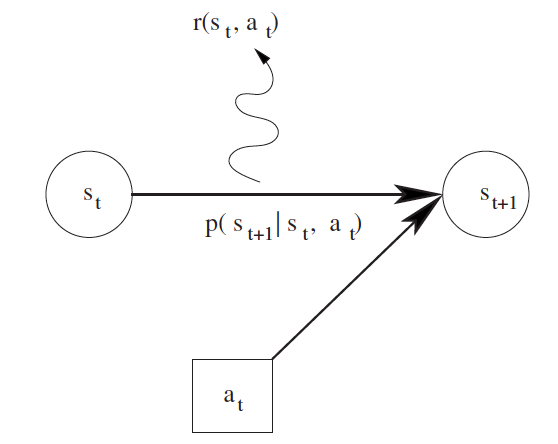
\includegraphics[width= 8cm, height = 7cm]{MDP.png}
	\caption{Markov decision process~\cite{Sigaud:2010:MDP:1841781}.}
	\label{fig:MDP}
\end{figure}

Markov decision processes allow to model the state evolution dynamics of a stochastic system when this system is controlled by an agent choosing and applying the actions $a_t$ at every time step $t$. The procedure of choosing such actions is called an action policy, or strategy, and is written as $\pi$~\cite{Sigaud:2010:MDP:1841781}.

\paragraph{Policy} Formally, given an MDP $\bigl\langle S, A, p(), R() \bigr\rangle$, a policy is a computable function that outputs for each state $s \in S$ an action $a \in A(s)$~\cite{wiering2012reinforcement}. A policy can decide deterministically upon the action to apply or can define a probability distribution over the possible applicable actions. Then, a policy can be based on the whole history $h_t$ (history-dependent policy) or can only consider the current state $s_t$. Thus, four main families of policies can be defined (\ref{table:T1}).

\begin{table}[h!]
\centering
\begin{tabular}{|c|c|c|}
	\hline \textbf{Policy $\pi_t$}
	&\textbf{Deterministic} & \textbf{Stochastic}  \\ 
	\hline
	\hline Markov 
	&$s_t \rightarrow a_t$  &$a_t, s_t \rightarrow [0, 1]$ \\ 
	 \hline History-dependent
	&$h_t \rightarrow a_t$  &$h_t, s_t \rightarrow [0,1]$  \\ 
	\hline
\end{tabular}
\caption{Different policy families for MDPs~\cite{Sigaud:2010:MDP:1841781}}
\label{table:T1}
\end{table} 

For a deterministic policy, $\pi_t (s_t)$ or $\pi_t (h_t)$ defines the chosen action $a_t$. For a stochastic policy, $\pi_t (a, s_t)$ or $\pi_t (a, h_t)$ represents the probability of selecting $a \in A$ for $a_t$~\cite{Sigaud:2010:MDP:1841781}. The sets so defined are included in each other, from the most general case of stochastic, history-dependent policies, to the very specific case of deterministic, Markov policies, as shown in figure \ref{fig:Policies_schema}.

\begin{figure}[h!]
	\centering
	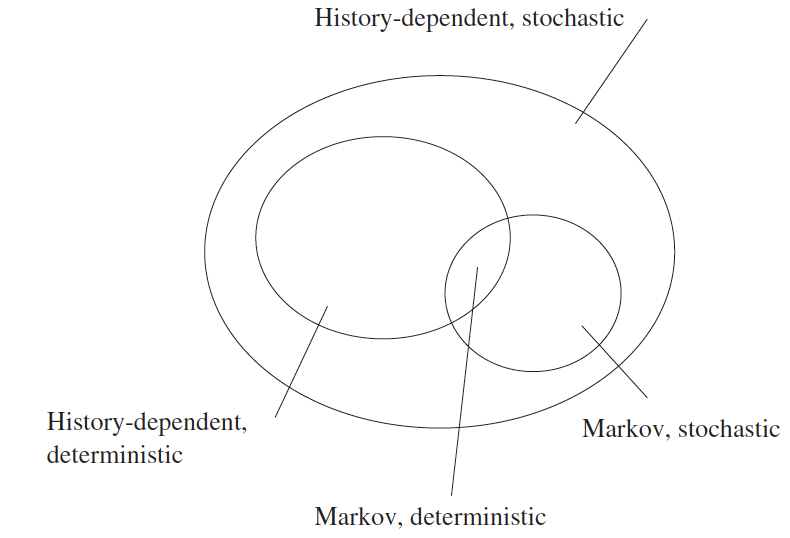
\includegraphics[width= 9cm, height = 8.5cm]{Policies_schema.png}
	\caption{Relationship between the different sets of policies~\cite{Sigaud:2010:MDP:1841781}.}
	\label{fig:Policies_schema}
\end{figure}

As shown in figure \ref{fig:Policy_application_schema} each time an agent performs an action $a\textsubscript{t}$ in a state $s\textsubscript{t}$, it receives a real-valued reward $r\textsubscript{t}$ that indicates the immediate value of this state-action transition. This produces a sequence of states $s\textsubscript{i}$, actions $a\textsubscript{i}$, and immediate rewards $r\textsubscript{i}$ as shown in the figure. The agent's task is to learn a control policy, $\{\pi : S \longrightarrow A\}$, that maximizes the expected sum of these rewards, with future rewards discounted exponentially by their delay~\cite{Mitchell}.

\begin{figure}[h!]
	\centering
	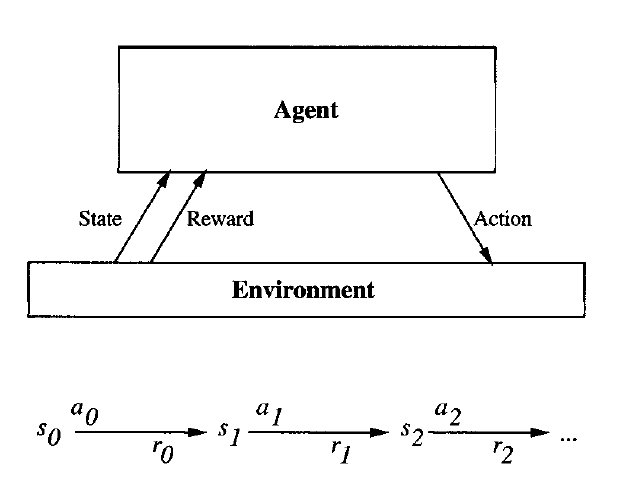
\includegraphics[width= 12cm, height = 10cm]{RLSchema.png}
	\caption{Policy application schema~\cite{SuttonBarto}.}
	\label{fig:Policy_application_schema}
\end{figure}
 
As previously said, the final goal of an optimal policy is to gather the greatest reward possible. In MDPs, there are several ways of taking into account the future in the current behaviour but there are basically three models of optimality which are sufficient to cover most of the approaches in the literature :

\begin{figure}[h!]
\begin{equation*}
E[\sum_{t = 0}^h r_t]
\qquad
E[\sum_{t = 0}^\infty \gamma^t r_t]
\qquad
\lim\limits_{h \rightarrow \infty} E[1/h \sum_{t = 0}^h r_t]
\end{equation*}
\caption{Optimality : \textbf{a)} finite horizon, \textbf{b)} discounted, infinite horizon, \textbf{c)} average reward}
\end{figure}

\paragraph{Discount Factor}The \textit{finite horizon} model simply takes a finite horizon of length $h$ and states that the agent should optimize its expected reward over this horizon. In the \textit{infinite-horizon model}, the long-run reward is taken into account, but the rewards that are received in the future are discounted according to how far away in time they will be received.
A \textit{discount factor} $\gamma$, with $0 \leq \gamma \leq 1$ is used for this. Note that in this discounted case, rewards obtained later are discounted more than rewards obtained earlier. Additionally, the discount factor, ensures that, even with infinite horizon, the sum of the rewards obtained is finite. In episodic tasks, i.e. in tasks where the horizon is finite, the discount factor is not
needed or can equivalently be set to $1$. If $\gamma = 0$ the agent is said to be myopic, which means that it is only concerned about immediate rewards.
The last optimality model is \textit{average-reward} model, maximizing the long-run \textit{average-reward}. Sometimes this is called the \textit{gain optimal} policy and in the limit, it is equal to the infinite-horizon discounted model~\cite{wiering2012reinforcement}

\subsection {Bellman Equation} The concept of \textit{value function} is the link between optimality criteria and policies. Most learning algorithms for MDPs compute optimal policies by learning value functions. The value of a state $s$ under policy $\pi$, denoted $V^\pi (s)$ is the expected return when starting in $s$ and following $\pi$ thereafter. Using the infinite-horizon, discounted model :

\begin{equation}
	V^\pi (s) = E_\pi \{\sum_{k = 0}^{\infty} \gamma^k r\textsubscript{t+k} | s_t = s\}
\end{equation}

A similar state-action value function : $Q : S$ x $A \rightarrow \mathbb{R}$ can be defined as the expected return starting from state $s$, taking action $a$ and thereafter following policy $\pi$ :

\begin{equation} \label{eq:2.2}
	Q^\pi (s,a) = E_\pi\{\sum_{k = 0}^{\infty} \gamma^k r\textsubscript{t+k} | s_t = s, a_t = a\}
\end{equation}

For any policy $\pi$ and any state $s$ the expression \ref{eq:2.2} can recursively be defined in terms of a so-called \textit{Bellman Equation} :

\begin{equation}
\begin{split}
	V^\pi (s) = E_\pi\{r_t + \gamma\textsubscript{t+1} + \gamma^2 r\textsubscript{t+2} + ... | s_t = t\} \\
	= E_\pi \{r_t + \gamma V^\pi(s\textsubscript{t+1}) | s_t = s\} \\
	\sum_{s'}p(s, \pi(s), s') (R(s, a, s') + \gamma V^\pi (s'))
\end{split}	
\end{equation}

It denotes that the expected value of state is defined in terms of immediate reward and values of possible next state weighted by the transition probabilities, and additionally a discount factor. Note that multiple policies can have the same value function, but for a given policy $\pi$, $V^\pi$ is unique. The goal for any MDP is to find a best policy, i.e. the policy that receives the most reward. This means maximizing the value function of equation \ref{eq:2.2} for all states $s \in S$. An optimal policy, denoted $\pi^*$, is such that $V\textsuperscript{$\pi$*} (s) \geq V^\pi (s)$ for all $s \in S$ and all policies $\pi$ :

\begin{equation} 
\label{eq:2.5}
V^*(s) = \max_{a \in A} \sum_{s'}p(s, \pi(s), s') (R(s, a, s') + \gamma V^\pi (s'))
\end{equation}

This expression is called the \textit{Bellman optimality equation}. It states that the value of a state under an optimal policy must be equal to the expected return for the best action in a state~\cite{wiering2012reinforcement}.

\subsection{Value Iteration vs Policy Iteration} Before studying how to solve MDPs let's clarify main differences between two key concepts that will be recursively find : \textit{value iteration} and \textit{policy iteration}. \\

Both value iteration and policy iteration compute the same thing (all optimal values), i.e. they work with Bellman updates. In value iteration one starts with a random value function and then he finds a new (improved) value function in an iterative process, until reaching the optimal value function. Value iteration computation of Bellman Equation is:

\begin{equation}
	V\textsubscript{k+1}(s) \leftarrow \max_{a} \sum_{s'} p(s, a, s') [R(s, a, s') + \gamma V_k(s')]
\end{equation}

\begin{figure}[h!]
	\centering
	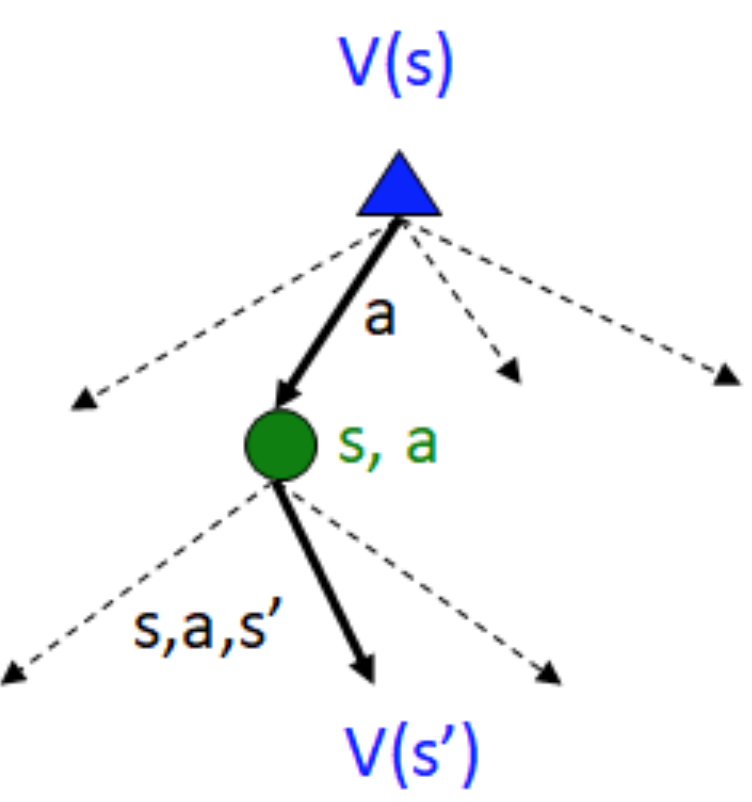
\includegraphics[width= 5cm, height = 5cm]{ValueIterationPolicy.png}
	\caption{Value Iteration Schema}
	\label{fig:ValueiterationPolicy}
\end{figure}

Value iteration has three disadvantages: it is slow ($O(S^2A)$ per iteration), the $\max$ at each state rarely changes, the policy often converges long before the values (figure \ref{fig:ValueiterationPolicy}). \\

Instead, policy iteration computations of Bellman Equation are:

\begin{itemize}
	\item Evaluation : for a fixed current policy $p$, find values with policy evaluation:
		\begin{equation}
			V\textsupsub{$\pi_i$}{$k+1$}(s) \leftarrow \sum_{s'}p(s, \pi_i(s), s')[R(s, \pi_i(s), s') + \gamma V\textsupsub{$\pi_i$}{k}(s')]
		\end{equation}
	
	\item Improvement : for fixed values, get a better policy using policy extraction :
	
	\begin{equation}
		\pi\textsubscript{i+1}(s) = \arg \max_{a} \sum_{s'} p(s, a, s')[R(s, a, s') + \gamma V\textsuperscript{$\pi_i$}(s')]
	\end{equation}
\end{itemize}

\begin{figure}[h!]
	\centering
	\includegraphics[width= 5cm, height = 5cm]{Policyiteration.png}
	\caption{Policy Iteration Schema}
	\label{fig:PolicyIteration}
\end{figure}

Complexity of policy iteration is $O(S^2)$. \\

Summarizing what said until now it is possible to write: \\ 

In value iteration :

\begin{itemize}
	\item Every iteration updates both the values and implicitly the policy;
	\item The policy is not tracked, but tacking the $\max$ over actions implicitly recomputes it.
\end{itemize}

In policy iteration :

\begin{itemize}
	\item Several passes that update utilities with fixed policy are made;
	\item After the policy is evaluated, a new policy is chosen;
	\item The new policy will be always better until the end.
\end{itemize}

\section{Solving MDP}
Now that the concepts of MDP, policy, optimality criteria and value function, have been formally defined, it is time to consider the question of how to solve an MDP computing an optimal policy $\pi^*$. Several dimensions exists along which algorithms have been developed for this purpose. The most important distinction is that between \textit{model-based} and \textit{model-free} algorithms ~\cite{wiering2012reinforcement}.

\begin{table}[h!]
	\resizebox{\textwidth}{!}{ 
		\begin{tabular}{|c|| c|c|}
			\hline 
			&\textbf{Model-based algorithms}  &\textbf{Model-free algorithms}  \\ 
			\hline
			\hline \textbf{General name} 
			&DP  &RL  \\ 
			\hline \textbf{Basic assumption} 
			&\thead{A model of the MDP is known \\ beforehand, and can be used to compute \\ value functions and policies using \\ the Bellman equation.}  &\thead{Rely on interaction with the environment. \\ Because a model of the MDP\\ is not known, the agent has\\ to explore the MDP to obtain information.}  \\
			\hline \textbf{Planning} 
			&Yes  &Yes  \\ 
			\hline \textbf{Learning} 
			&No  &Yes  \\ 
			\hline 
		\end{tabular} 
	}
	\caption{Main differences between model-based and model-free algorithms.}
\end{table}

\subsection{Dynamic Programming} The term Dynamic Programming (DP) refers to a class of algorithms that is able to compute optimal policies in the presence of a perfect model of the environment described as a Markov Decision Process. These algorithms are known as \textit{planning algorithms}. In planning, the idea is that some description of a starting state or states, a goal state or states, and some set of possible actions that the agent can take are given. The objective is to search through a tree that is the sequences of actions that can be taken, and try to find a nice short plan. In so doing two of the possible planning algorithms are {\tt BFS algorithm} and {\tt DFS algorithm}. \\

The method of Dynamic Programming systematically records solutions for all sub-problems of increasing lengths. Using this programming paradigm the optimal policy is constructed through the step-by-step definition of optimal sub-policies. According to Bellman optimality principle, all optimal sub-policies of an optimal policy are optimal sub-policies. DP algorithms are obtained by turning Bellman equations into update rules for improving approximations of the desired value functions.

Studying DP it is possible to distinguish two different main methods. \textit{Policy evaluation} refers to the typically iterative computation of the value functions for a given policy. \textit{Policy improvement} refers to the computation of an improved policy given the value function for that policy. Either of these can be used to reliably compute optimal policies and value functions for finite MDPs given complete knowledge of the MDP.


Classical DP methods operate in sweeps through the state set, performing an \textit{expected update} operation on each state. Each such operation updates the value of one state based on the values of all possible successor states and their probabilities of occurring. Expected updates are closely related to Bellman equations: they are little more than these equations turned into assignment statements. When the updates no longer result in any changes in value, convergence has occurred to values that satisfy the corresponding Bellman equation~\cite{SuttonBarto}. \\

The assumption that a model is available will be hard to ensure for many applications, however DP algorithms are very relevant because they define fundamental computational mechanism which are also used when no model is available. 

\subsection{Reinforcement Learning}
Dynamic Programming' s methods compute optimal policies for an MDP assuming that a perfect model is available. Reinforcement Learning (or \textit{approximate dynamic programming}, or \textit{neuro-dynamic programming}) is primarily concerned with how to obtain an optimal policy when such a model is not available. RL adds to MDPs a focus on approximation and incomplete information, and the need for sampling and exploration. In contrast with DP's algorithms, model-free methods do not rely on the availability of priori known transition and reward models. The lack of the model generates a need to \textit{sample} the MDP to gather statistical knowledge about this unknown model. Many model-free RL techniques exist that probe the environment by doing actions, thereby estimating the same kind of state value and state-action value functions as model-based techniques~\cite{wiering2012reinforcement}.\\

Roughly speaking Reinforcement Learning (RL) is the problem faced by a learner that must behaviour through trial-and-error interactions with a dynamic environment. It can be considered a problem of mapping situations to actions in order to maximize a numerical reward signal~\cite{RLDef1}. \\

In RL the learner must select an action to take in each time step: every choice done by the agent changes the environment in an unknown fashion and receives a reward which value is based on the consequences. The objective of the learner is to choose a sequence of actions based on observations of the current environment that maximizes cumulative reward or minimizes cumulative cost over all time steps~\cite{LiMalik}. The general class of algorithms that interact with the environment and update their estimates after each experience is called \textit{online} RL.

\begin{algorithm}
	\ForEach{episode}{
		$s \in S$ is initialized as the starting state\;
		$t := 0$\;
		\Repeat{$s'$ is a goal state}{
			choose an action $a \in A(s)$\;
			perform action $a$ \;
			observe the new state $s'$ and received reward $r$ update $\tilde{T}, \tilde{R}, \tilde{Q}$ and/or $\tilde{V}$ using the experience $\bigl \langle$$s, a, r, s'$$\bigr\rangle$\;
			$s:=s'$\;
		}
		
	}
	\caption{A general algorithm for online RL~\cite{wiering2012reinforcement}}
\end{algorithm}

Studying RL, one of the main aspect is the distinction between \textit{direct} and \textit{indirect} Reinforcement Learning. The difference between these two approaches is shown in figure \ref{tab:RL_possibilities_schema}. \\

\begin{table}[h!]
	\resizebox{\textwidth}{!}{ 
		\begin{tabular}{|c|| c|c|}
			\hline 
			&\textbf{Model-based/Indirect}  &\textbf{Model-free/Direct}  \\ 
			\hline
			\hline \textbf{Basic Assumption} 
			& \thead{First of all it is necessary \\ to learn the transition and \\ reward model from interaction \\ with the environment. After that, when \\ the model is (approximately or sufficiently) \\ correct, all the DP methods previously described \\ can be applied. } & \thead{It is possible to estimate \\ values of functions, without even \\ estimating the model of the MDP.}  \\ 
			\hline 
		\end{tabular} 
	}
	\caption{RL's approaches classification.}
	\label{tab:RL_possibilities_schema}
\end{table}

RL is different both from \textit{supervised learning} and from \textit{unsupervised learning}. It is not a sample of learning from a training set of labelled examples provided by a knowledgeable external supervisor (\textit{supervised learning}) and it is not a sample of searching and finding structure hidden in a collection of unlabelled data (\textit{unsupervised learning}). More specifically RL can be distinguished from other forms of learning based on the following characteristics :

\begin{itemize}
	\item Reinforcement Learning deals with temporal sequences. In contrast with non-supervised learning problems where the order in which the examples are presented is not relevant, the choice of an action at a given time step will have consequences on the examples that are received at a subsequent time steps~\cite{Sigaud:2010:MDP:1841781}.
	\item In contrast with supervised learning, the environment does not tell the agent what would be the best possible action. Instead, the agent may just receive a scalar reward representing the value of its action and it must \textit{explore} the possible alternative actions to determine whether its action was the best or not~\cite{Sigaud:2010:MDP:1841781}.
\end{itemize}

According to what just said, one of the challenges that arise in RL, and not in other kind of learning, is the trade-off between \textit{exploration} and \textit{exploitation}. To obtain an higher reward, an RL agent must prefer actions that it has tried in the past and found to be effective in producing reward. In order to discover such actions, it has to try actions that it has not selected before. The agent \textit{exploits} what it has already experienced in order to obtain reward, but it has also to \textit{explore} in order to eventually make better action selections in the future~\cite{SuttonBarto}. In other words \textit{exploitation} consists of doing again actions which have proven fruitful in the past, whereas \textit{exploration} consists of trying new actions, looking for a larger cumulated reward, but eventually leading to a worse performance. Dealing with the exploration/exploitation trade-off consists of determining how the agent should explore to get as fast as possible a policy that is optimal or close enough to the optimum. The most basic exploration strategy is the $\epsilon$-greedy policy, i.e. the learner takes its current best action with probability $(1-\epsilon)$ and a (randomly selected) other action with probability $\epsilon$. ~\cite{Sigaud:2010:MDP:1841781}. 

\subsection{Monte Carlo Methods} Monte Carlo Methods (MC)  represent a first instance of model-free RL's algorithms. They are one way solving the Reinforcement Learning problem based on averaging sample returns.

The Monte Carlo approach consists of performing a large number of trajectories from all states $s$ in $S$, and estimating $V(s)$ as an average of the cumulated rewards observed along these trajectories. In each trial, the agent records its transitions and rewards, and updates the estimates of the value of the  encountered states according to a discounted reward scheme. The value of each state then converges to $V^\pi (s)$ for each $s$ if the agent follows policy $\pi$.

More formally, let $(s_0, s_1, ..., s_N)$ be a trajectory consistent with the policy $\pi$ and the unknown transition function $p()$, and let $(r_1, ..., r_N)$ be the rewards observed along this trajectory. In MC method, the $N$ values $V(s_t), \quad t = 0, ...., N-1$ are updated according to :

\begin{equation} 
\label{eq:2.6}
V(s_t) \leftarrow V(s_t) + \alpha(s_t)(r\textsubscript{t+1} + r\textsubscript{t+2} + ... + r_N - V(s_t))
\end{equation}

with the learning rates $\alpha(s_t)$ converging to $0$ along the iterations~\cite{Sigaud:2010:MDP:1841781} . MC algorithms treat the long-term reward as a random variable and take as its estimate the sampled mean. Because the sampling is dependent on the current policy $\pi$, only returns for actions suggested by $\pi$ are evaluated. Thus, \textit{exploration} is of key importance here, just as in other model-free methods. One way of ensuring enough exploration is to use exploring starts, i.e. each state-action pair has a non-zero probability of being selected as the initial pair.

A distinction can be made between \textit{every-visit} MC, which averages over all visits of a state $s \in S$ in all episodes, and \textit{first-visit} MC, which averages over just the returns obtained from the first visit to a state $s \in S$ for all episodes. Both variants will
converge to $V^\pi$ for the current policy $\pi$ over time~\cite{wiering2012reinforcement} .

Studying RL methods it is necessary to distinguish between \textit{on-policy methods} and \textit{off-policy methods}.
On-policy methods attempt to evaluate or improve the policy that is used to make decisions. Off-policy methods evaluate or improve a policy different from that used to generate the data. MC methods can be used for both on-policy and off-policy control, and the general pattern complies with the generalized policy iteration procedure. 

\begin{table}
\centering
\begin{tabular}{|c|c|c|}
	\hline 
	&\textbf{On-policy methods}  &\textbf{Off-policy methods}  \\ 
	\hline \textbf{Basic assumption}
	& \thead{They attempt to evaluate\\ or improve the policy that\\ is used to make decisions.}  &\thead{No specific policy \\ is required to be followed; \\ the agent could \\ even behave randomly and \\ despite this it can still  \\ find the optimal policy. }  \\ 
	\hline 
\end{tabular}
\caption{Difference between on-policy and off-policy methods.}
\end{table} 

\subsection{Temporal Difference Learning} An important problem faced by RL is the so called \textit{temporal credit assignment problem}. In model-free contexts it is difficult to assess the utility of some action, if the real effects of this particular action can only be perceived much later. One possibility is to wait until the ”end” (e.g. of an episode) and punish or reward specific actions along the path taken. However, this will take a lot of memory and often, with ongoing tasks, it is not known beforehand whether, or when, there will be an ”end”. Instead, one can use similar mechanisms as in value iteration to adjust the estimated value of a state based on the immediate reward and the estimated (discounted) value of the next state. This is generally called \textit{temporal difference learning} which is a general mechanism underlying the model-free methods~\cite{wiering2012reinforcement}. \\ 

The basic temporal difference algorithm is $TD(0)$. This algorithm relies on a comparison between the actually received reward and the reward expected from the previous estimations.

If the estimated values $V(s_t)$ and $V(s\textsubscript{t+1})$ in states $s_t$ and $s\textsubscript{t+1}$ were exact, one would have 

\begin{equation}
	V(s_t) = r\textsubscript{t+1} + \gamma r\textsubscript{t+2} + \gamma^2 r\textsubscript{t+3} + ...,
\end{equation}

\begin{equation}
	V(s\textsubscript{t+1}) = r\textsubscript{t+2} + \gamma r\textsubscript{t+3} + \gamma^2r\textsubscript{t+4} + ... .
\end{equation}

Thus one would have 

\begin{equation}
	V(s_t) = r\textsubscript{t+1} + \gamma V(s\textsubscript{t+1}).
\end{equation}

The temporal difference error

\begin{equation}
	\delta_t = r\textsubscript{t+1} + \gamma V(s\textsubscript{t+1}) - V(s_t)
\end{equation}

measures the error between the current estimation $V(s_t)$ and the corrected estimation $r\textsubscript{t+1} + V(s\textsubscript{t+1})$. The temporal difference method consists of correcting this error little by little by modifying $V()$ according to a Windrow-Hoff equation :

\begin{equation}
	V(s_t) \leftarrow V(s_t) + \alpha[r\textsubscript{t+1} + \gamma V(s\textsubscript{t+1}) - V(s_t)] = V(s_t) + \alpha \delta_t .
\end{equation}

Like Monte Carlo methods, TD ones perform estimation of action-value functions based on the experience of the agent and can do it without a model of the underlying MDP; however, they combine this estimation using local estimation propagation mechanisms coming from dynamic programming, resulting in their incremental properties. Thus TD methods, which are at the heart of most reinforcement learning algorithms, are characterized by this combination of estimation methods with local updates incremental properties~\cite{Sigaud:2010:MDP:1841781}.

\subsection{Sarsa Algorithm : On-policy TD Control} Knowing the exact value of all states is not always enough to determine what to do. If the agent does not know which action results in reaching any particular state, i.e. if the agent does not have a model of the transition function, knowing $V$ does not help it determine its policy.  To solve this problem, Watkins ~\cite{watkins1992q} introduced the action-value function $Q$, whose knowledge is similar to the knowledge of $V$ when $p$ is known. The action-value function of a fixed policy $\pi$ whose value function is $V^\pi$ is :

\begin{equation}
	\forall s \in S, a \in A, \quad Q^\pi (s,a) = R(s, a) + \gamma \sum_{s'} p(s' \ s, a) V^\pi (s').
\end{equation}

The value of $Q^\pi(s,a)$ is interpreted as the expected value when starting from $s$, executing $a$ and then following the policy $\pi$ afterwards. Having $V^\pi(x) = Q^\pi(x, \pi(x))$, the corresponding Bellman equation is :

\begin{equation}
	\forall s \in S, a \in A \quad Q^*(s, a) = R(s, a) + \gamma \sum_{s'}p(s' | s, a) \max_{b} Q^*(s', b)
\end{equation}

Than :

\begin{equation}
\forall s \in S, \quad V^*(s) = \max_{a} Q^* (s,a ), \quad \pi^*(s) = \arg\max_{a} Q^*(s,a).
\end{equation}

The SARSA algorithm works on state-action pairs rather than on states. Its update equation is :

\begin{equation}
\label{eq:2.12}
Q(s_t, a_t) \leftarrow Q(s_t, a_t) + \alpha[r\textsubscript{t+1} + \gamma Q(s\textsubscript{t+1}, a\textsubscript{t+1}) - Q(s_t, a_t)].
\end{equation}

the information necessary to perform such an update is $(s_t, a_t, r\textsubscript{t+1}, s\textsubscript{t+1}, a\textsubscript{t+1})$, hence the name of the algorithm : SARSA. This algorithm suffers from one conceptual drawback: performing the updates as stated above implies knowing in advance what will be the next action $a\textsubscript{t+1}$ for any possible next state $s\textsubscript{t+1}$.  As a result, the learning process is tightly coupled to the current policy (the algorithm is called "on-policy") and this complicates the exploration process. As a result, proving the convergence of SARSA was more difficult than proving the convergence of "off-policy" algorithms such as Q-learning. Empirical studies often demonstrates the better performance of SARSA compared to Q-learning~\cite{Sigaud:2010:MDP:1841781}.

\begin{algorithm}
	Initialize $Q(s, a)$ arbitrarily\;
	Repeat the next cycle until $s$ is terminal\;
	\ForEach{epsiode}{
	Initalize $s$\;
	Choose $a$ from $s$ using policy derived from $Q$ (e.g. $\epsilon$-greedy)\;
	\ForEach{step of episode}{
		Take action $a$, observer $r$, $s'$\;
		Choose $a'$ from $s'$ using policy derived from $Q$ (e.g. $\epsilon$-greedy)\;
		$Q(s,a) \leftarrow Q(s,a) + \alpha[r + \gamma Q(s', a') - Q(s, a)]$ \;
		$s \leftarrow s'$ \;
		$a \leftarrow a'$ \;
	}
} 
\caption{SARSA Algorithm : On-policy TD Control}
\end{algorithm}

\subsection{Q-learning Algorithm : Off-policy TD Control} The Q-Learning Algorithm can be seen as a simplification of the  algorithm, given that it is no more necessary to determine the action at the next step to calculate updates. Its update equation is :

\begin{equation}
\label{eq:2.13}
	Q(s_t, a_t) \leftarrow Q(s_t, a_t) + \alpha[r\textsubscript{t+1} + \gamma \max_{a} Q(s\textsubscript{t+1}, a) - Q(s_t, a_t)]
\end{equation} 

\begin{algorithm}
	$\alpha_t$ is the learning rate \;
	Initialize ($Q_0$)\;
	\For{$t = 0$ ; $t \leq T\textsubscript{tot} - 1$ ; $t++$}{
		$s_t \leftarrow {\tt ChooseState}$\;
		$a_t \leftarrow {\tt ChooseAction}$\;
		$s\textsubscript{t+1}, r\textsubscript{t+1} \leftarrow {\tt Simulate}(s_t, a_t)$\;
		update $Q_t$ \;
		\Begin{
			$Q\textsubscript{t+1} \leftarrow Q_t$\;
			$\delta_t \leftarrow r\textsubscript{t+1} + \gamma \max_{b} Q_t (s\textsubscript{t+1}, b) - Q_t(s_t, a_t)$ \;
			$Q\textsubscript{t+1}(s_t, a_t) \leftarrow Q_t(s_t, a_t) + \alpha_t(s_t, a_t) \delta_t$ \;
		}
	}
\KwRet{Q\textsubscript{Tot}}
\caption{Q-learning Algorithm ~\cite{Sigaud:2010:MDP:1841781}}
\end{algorithm}

The main difference between SARSA and Q-Learning lies in the definition of the error term. The $Q(s\textsubscript{t+1}, a\textsubscript{t+1})$ term in the equation \ref{eq:2.12}	is replaced by $\max_{a}Q(s\textsubscript{t+1}, a)$ in equation \ref{eq:2.13}. Updates are based on instantaneously available information. In this algorithm, the $T\textsubscript{tot}$ parameter corresponds to the number of iterations. There is here one learning rate $\alpha_t(s, a)$ for each state-action pair, it decreases at each visit of the corresponding  pair. The {\tt Simulate} function returns a new state and the corresponding reward according to the dynamics of the system. The choice of the current state and of the executed action is performed by functions {\tt ChooseState} and {\tt ChooseAction}. The {\tt Initialize} function initializes the $Q$ function with $Q_0$, which is often initialized with {\tt null} values, whereas more adequate choices can highly improve the performance~\cite{Sigaud:2010:MDP:1841781}.

\subsection{SARSA($\lambda$) Algorithm} Previous algorithms only perform one update per time step in the state that the agent is visiting. This update process is particularly slow. Indeed, an agent deprived of any information on the structure of the value function needs at least $n$ trials to propagate the immediate reward of a state to another state that is $n$ transitions away. Before this propagation is achieved, if the initial values are {\tt null}, the agent performs a random walk in the state space, which means that it needs an exponential number of steps as a function of $n$ before reaching the reward "trail" (figure \ref{fig:NonLambda}).

\begin{figure}[h!]
	\centering
	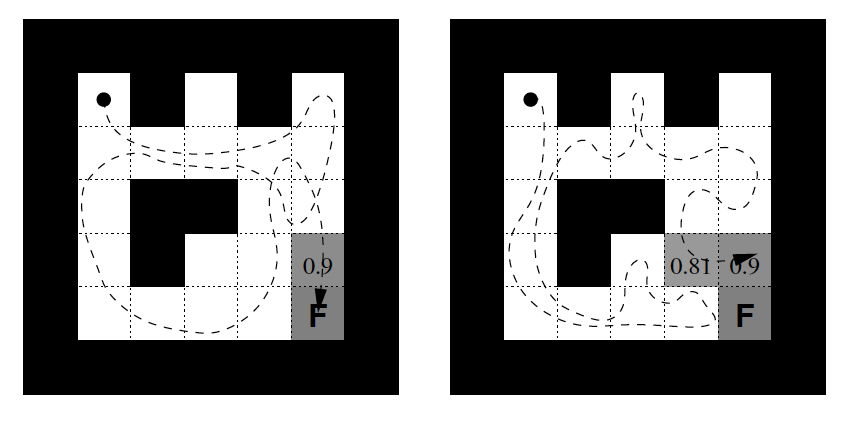
\includegraphics[width= 10cm, height = 5cm]{NonLambda}
	\caption{Q-learning : first and second trial. It can be seen that, all values being initially {\tt null}, the propagation of {\tt non-null} values does not starts until the agent finds the reward source for the first time, and only progress once per trial~\cite{Sigaud:2010:MDP:1841781}.}
	\label{fig:NonLambda}
\end{figure}

A naive way to solve the problem consists of using a memory of trajectory and to propagate all the information backwards along the performed transitions each time a reward is reached. Such a memory of performed transitions is called an ''eligibility trace''. A problem with this naive approach is that the required memory grows with length of trajectories, which is obviously not feasible in the infinite horizon context. In SARSA($\lambda$) algorithm a more sophisticated approach that addresses the infinite horizon context is used. \\

As already saw, Q-learning integrates the temporal difference error idea. With the update rule of Q-learning :

\begin{equation}
	Q\textsubscript{t+1} (s_t, a_t) = Q_t(s_t, a_t) + \alpha_t\{r\textsubscript{t+1} + \gamma V_t(s\textsubscript{t+1}) - Q_t(s_t, a_t)\}
\end{equation}

for transition ($s_t, a_t, s\textsubscript{t+1}, r\textsubscript{t+1}$), and in the case where action $a_t$ executed in state $s_t$ is the optima action for $Q_t$, then the error term is $r\textsubscript{t+1} + \gamma V_t s\textsubscript{t+1} - V_t(s_t)$. For a generic parameter $\lambda \in [0,1]$ it can be generalized as shown in algorithm \ref{SarsaLambdaAlgo}.

\begin{algorithm}
	/* $\alpha$ is a learning rate */ \;
	{\tt Initialize} $Q_0$ \;
	$z_0 \leftarrow 0$ \;
	$s_0 \leftarrow$ {\tt ChooseState} \;
	$a_0 \leftarrow$ {\tt ChooseAction} \;
	$t \leftarrow 0$ \;
	\While{$t \leq  T\textsubscript{tot}-1$}{
		($s_t', r\textsubscript{t+1}$) $\leftarrow$ {\tt Simulate} $(s_t, a_t)$ \;
		$a_t' \leftarrow$ {\tt ChooseAction} \;
		update $Q_t$ and $z_t$ \;
		\Begin{
			$\delta_t \leftarrow r\textsubscript{t+1} + \gamma Q_t(s_t', a_t') - Q_t(s_t, a_t)$ \;
			$z_t(s_t, a_t) \leftarrow z_t(s_t, a_t) + 1$ \;
			\For{$s \in S, a \in A$}{
				$Q\textsubscript{t+1}(s, a) \leftarrow Q_t(s, a) + \alpha_t(s,a)z_t(s,a)\delta_t$ \;
				$z\textsubscript{t+1}(s,a) \leftarrow \gamma\lambda z_t(s,a)$
			}
		\If{$s_t'$ non absorbing}{
				$s\textsubscript{t+1} \leftarrow s_t'$ and $a\textsubscript{t+1} \leftarrow a_t'$ \;
			}
		\Else{
				$s\textsubscript{t+1} \leftarrow$ {\tt ChooseState} \;
				$a\textsubscript{t+1} \leftarrow$ {\tt ChooseAction} \;
			}
		}
	}
\KwRet{$Q\textsubscript{Tot}$}
\caption{SARSA ($\lambda$) Algorithm \cite{Sigaud:2010:MDP:1841781}}
\label{SarsaLambdaAlgo} 
\end{algorithm}

Here $z_t(s, a)$  is the eligibility trace and \textit{absorbing state} is the terminal state~\cite{Sigaud:2010:MDP:1841781}. The eligibility trace represents a short-term memory vector, \textbf{z\textsubscript{t}} $\in \mathbb{R}^d$, that parallels the long-term weight vector \textbf{w\textsubscript{t}} $\in \mathbb{R}^d$. The rough idea is that when a component of \textbf{w\textsubscript{t}} participates in producing an estimated value, then the  corresponding component of \textbf{z\textsubscript{t}} is bumped up and then begins to fade away. Learning will then occur in that component of \textbf{w\textsubscript{t}} if a non-zero TD error occurs before the trace falls back to zero. The trace-decay parameter $\lambda \in [0, 1]$ determines the rates at which the trace falls \cite{SuttonBarto}. Roughly speaking eligibility trace is a parameter used to control the “memory” of the algorithm, associated to a given state, enabling the assignment of more credit, i.e., higher trace, to the states and actions performed closer to the end of the episode.

\begin{figure}[h!]
	\centering
	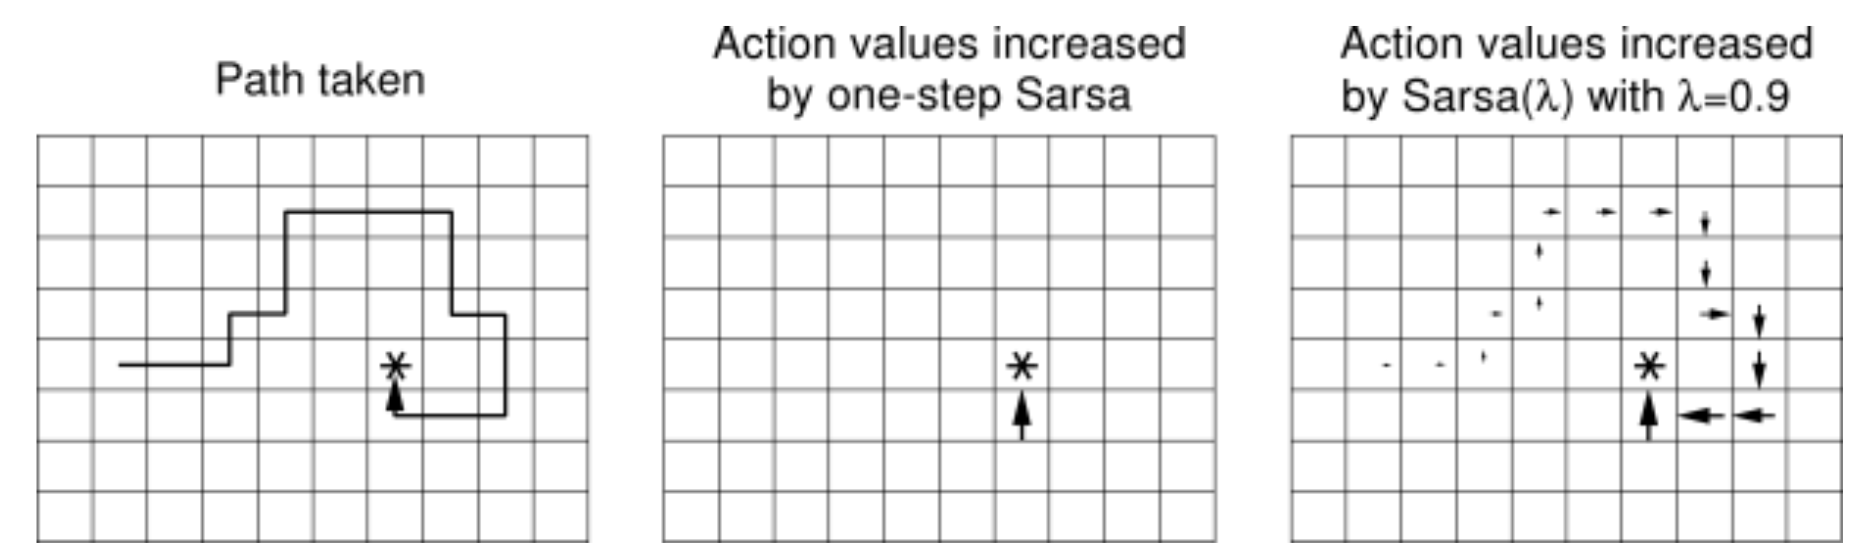
\includegraphics[width= 12cm, height = 5cm]{SarsaLambdaTD}
	\caption{Grid-world example of the speed up of policy learning due to the use of eligibility traces.}
	\label{fig:SarsaLambdaTD}
\end{figure}

The effect of the $\lambda$ value is still poorly understood and tuning optimally its value for a given problem is still an open empirical problem \cite{Sigaud:2010:MDP:1841781}.



	\chapter{A Reinforcement Learning Approach to Black-Box Optimization}

One of the principal challenges in optimization practice is how to optimize in absence of an algebraic model of the system to be optimized. This kind of optimization is known as \textit{black-box optimization}. \\

A black-box function $f(x) : \mathbb{R}^n \rightarrow \mathbb{R}$ is a function for which the analytic form is not known. Nowadays there are lots of mathematical models to solve these type of functions. One of the best known of these methods is the \textit{Bayesian Optimization Model} (BO). \\
In this chapter we will first explain how BO works and than we will propose an innovative, RL based approach for black-box optimization problem.

\paragraph{Gaussian Processes} Before starting to speak about BO we have to describe what \textit{Gaussian Processes} (GPs) are. GPs are an alternative approach to regression problems. The GP approach is a \textit{non-parametric} (we don't have a priori knowledge of how many parameters will be useful for our regression) approach to find a distribution over the possible function $f(x)$ that are consistent with observed data. A GP is a generalization of the Gaussian probability distribution. Whereas a probability distribution describes random variables which are scalars or vectors (for multivariate distributions), a stochastic process governs the properties of functions.
GP is a convenient and powerful prior distribution on functions, which we will take here to be of the form $f : \mathcal{X} \leftarrow \mathbb{R}$. The GP is defined by the property that any finite set of $N$ points $\{x_n \in \mathcal{X}\}\subsup{}{ n=1}{N}$ induces a multivariate Gaussian distribution  on $\mathbb{R}^N$. The $n$th of these points is taken to be the function value $f(x_n)$. The support and properties of the resulting distribution on functions are determined by a mean function $m : \mathcal{X} \leftarrow \mathbb{R}$ and a positive definite covariance function $K : \mathcal{X} \times \mathcal{X} \leftarrow \mathbb{R}$ ~\cite{NIPS2012_4522}.

\begin{figure} [h!]
	\centering
	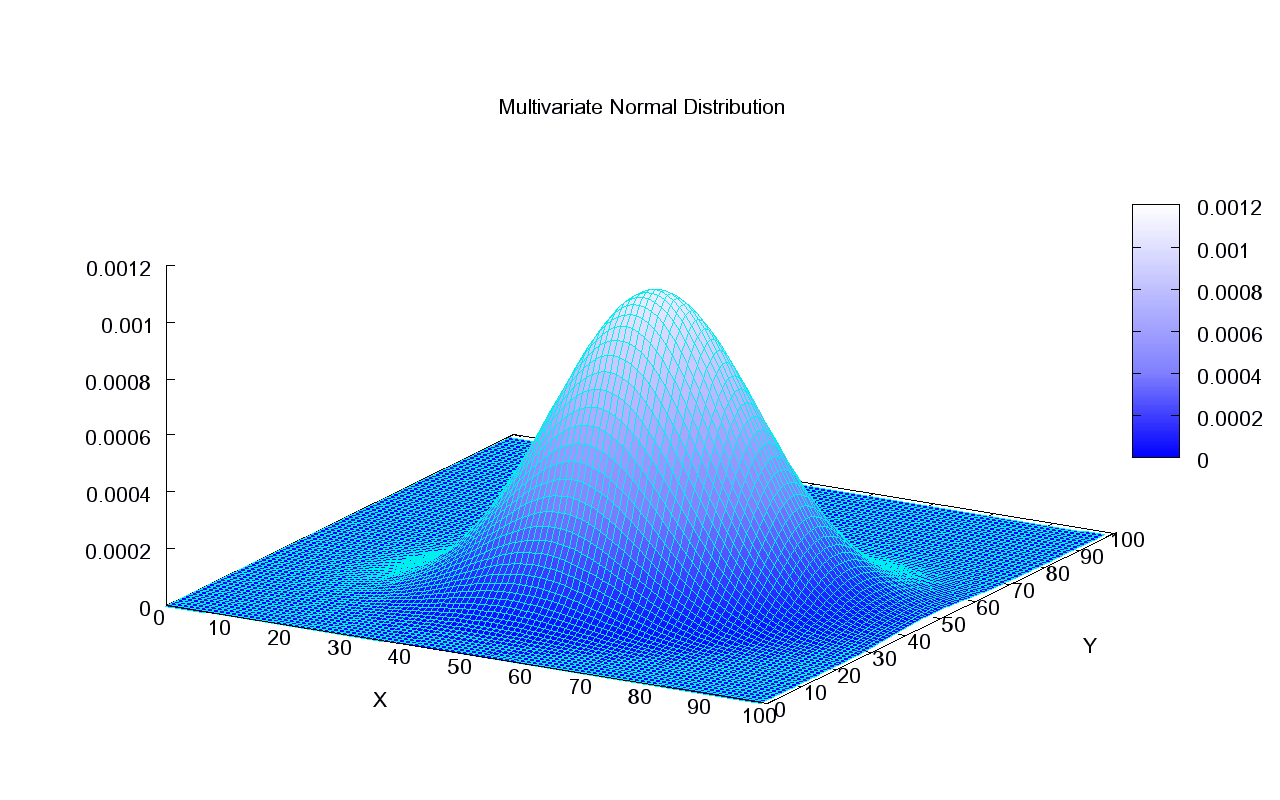
\includegraphics[width= \textwidth, height = 9.5cm]{Multivariate_Gaussian.png}
	\caption{Multivariate Gaussian Distribution [Wikipedia]}
	\label{fig:Multivatiate_Gaussian}
\end{figure}

\paragraph{Acquisition Functions for Bayesian Optimization} Let's assume that the function $f(x)$ is drawn from a GP prior and that our observation are of the form $\{x_n \in \mathcal{X}\}\subsup{}{ n=1}{N}$, where $y_n \sim \mathcal{N}(f(x_n), v)$ and $v$ is the variance of noise introduced into the function observations. This prior and these data induce  posterior over functions; the acquisition function, which we denote by $a : \mathcal{X} \leftarrow \mathbb{R}^+$, determines what point in $\mathcal{X}$ should be evaluated next via a proxy optimization $x\textsubscript{next} = \arg\max_{x}a(x)$, where several different functions have been proposed. There are several popular choices of acquisition function. Under the Gaussian process prior, these functions depend on the model solely through its predictive mean function $\mu(x; \{x_n, y_n\})$ and predictive variance function $\sigma^2(x; \{x_n, y_n\})$~\cite{NIPS2012_4522}.

\begin{figure} [h!]
	\centering
	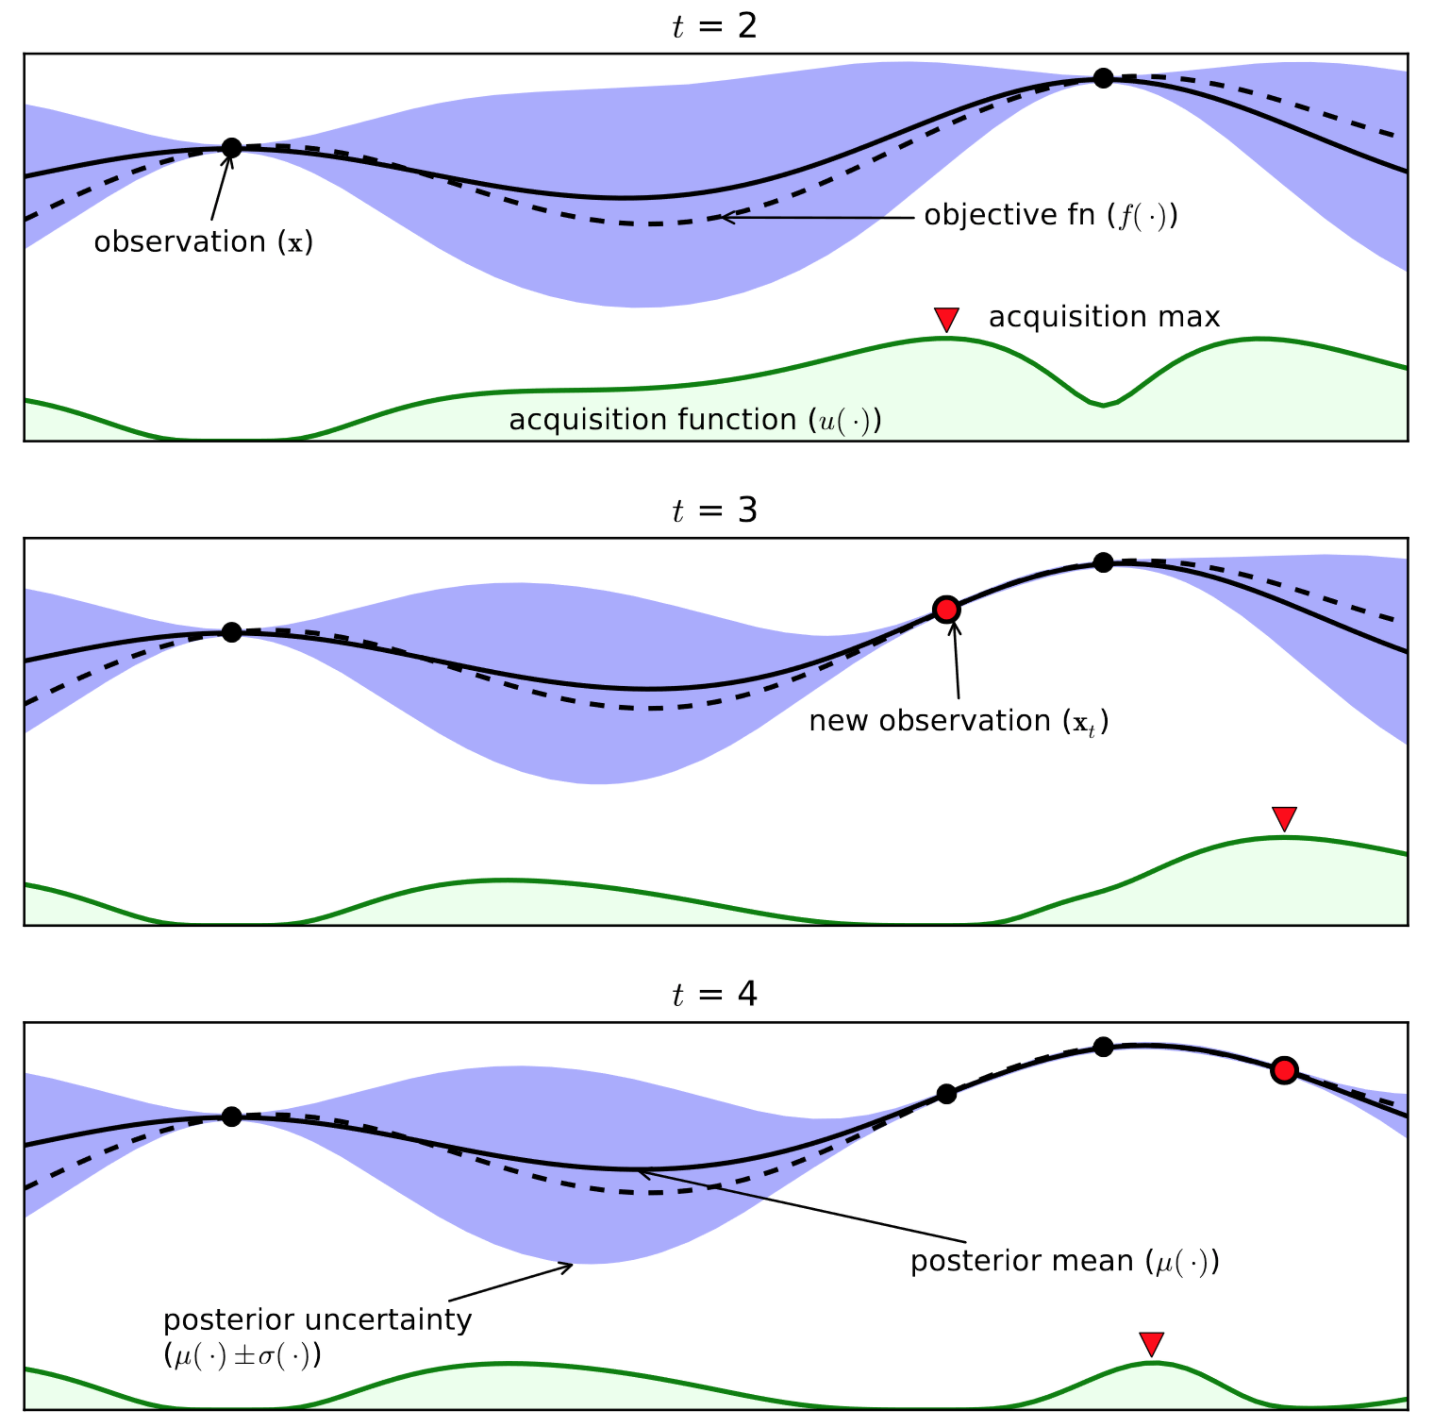
\includegraphics[width= \textwidth, height = 13cm]{BOProcess.png}
	\caption{2-$d$ Bayesian Optimization Process Example[towardsdatascience.com]}
	\label{fig:BoProcess}
\end{figure}

\paragraph{An RL Approach} As previously said in this thesis we describe an innovative RL approach to the black-box function optimization problem. Let's assume to dispose of a function $f(x, y)$. In our RL problem :

\begin{itemize}
	\item \textbf{Agent} : The agent has to maximize a black-box bivariate function. Each function is continuously defined over a specific domain. The agent has to complete its job making exactly $150$ epochs for each one of the $1000$ episodes. In each epoch it has a position in space described through the two coordinates $(x, y)$. Each time the agent makes an action the angle between $(x, y)$ and $(x', y')$ and the value of the function $f(x', y')$ are computed.
	\item \textbf{State} : The state is represented by two lists: the first one contains the last two computed \textit{angles} and the second one contains the correspondent last two \textit{actions}.
	\item \textbf{Actions} : In each epoch the agent can make one of four different actions : \textit{move north}, \textit{move  south}, \textit{move east}, \textit{move west}. Each time the agent moves itself of $40$ pixels in one of the previously described directions. The resultant effective movement is computed as follow:
	
	\begin{algorithm} [h!]
		/* knowing $pixelX$ and $pixelY$ */\;
		/* knowing $pixelXRange$ and $pixelYRange$ */ \;
		/* knowing $function$ */\;
		
		\
		
		$domain = function.getDomain()$ \;
		$xRange = domain.maxX - domain.minX$ \;
		$yRange = domain.maxY - domain.minY$ \;
		
		\
		
		$xReal = domain.minX + (pixelX * xRange) / pixelXRange$ \;
		$yReal = domain.minY + (pixelY * yRange) / pixelYRange$ \;
		
		\
		
		\KwRet{$xReal, yReal$}
		\caption{From pixels to real values} 
	\end{algorithm}
	
	\item \textbf{Reward} : In this context we have decided to reward every action of the agent because a real terminal state doesn't exist. Cause we are working with a black-box function we cannot select two coordinate $(x, y)$ and a corresponding value function $z$ as a terminal state. The simulation ends after $1000$ episodes are done. We define a $\Delta$ equals to $\max f(z_n)$ minus $f(z)$ computed in the \textit{current state}:
	
	\begin{equation}
		\Delta = max f(x_n, y_n) - f(x, y)
	\end{equation} 
	
	Our reward at each epoch is equal to $\Delta$.
\end{itemize}

The movement the agent can make in each epoch can be of two different types : \textit{linear movement} or \textit{parametric movement}. If the movement is linear we compute the angle as follow :

\begin{algorithm}
	/* knowing $(x, y)$ */ \;
	/* knowing $(x', y')$*/ \;
	/* {\tt movementAmount} = \textit{M} */ \;
	/* {\tt currentMax} = $\max f(x_n, y_n)$ */ \;
	
	
	\
	
	$z = f(x, y)$ \;
	$z' = f(x', y')$\;
	
	\
	
	$\delta = ((x'-x),  (y'-y))$ \;
	$\alpha = \arctan(\dfrac{\delta}{\tt movementAmount})$
	 
	 \
	 
	 $\Delta = $z'$ - {\tt currentMax} $
	 
	 \caption{Angle computation in linear movement case.} 
	
\end{algorithm}

We can explain this algorithm briefly recalling some trigonometry. Let's suppose to be in a simple 2d case like the one represented in figure ~\ref{fig:LMComputations}.

\begin{figure} [h!]
	\centering
	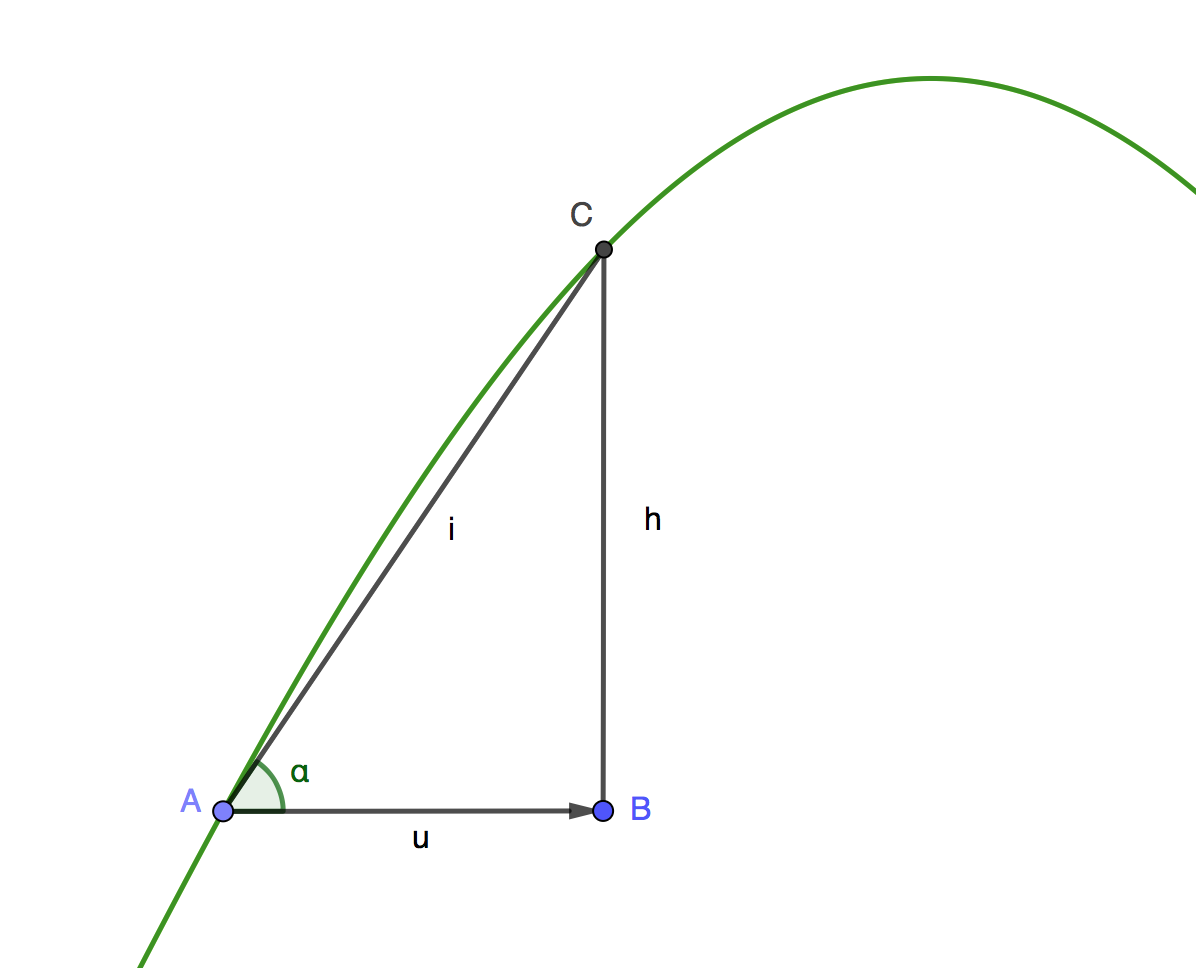
\includegraphics[width= 7cm, height = 7cm]{Triangolo.png}
	\caption{Linear movement computations.}
	\label{fig:LMComputations}
\end{figure}

Let's suppose that the starting point of our RL agent at epoch \textit{e} is the point \textit{A} with coordinates $(x, y)$. In the represented case the agent can make only one of two actions for each epoch : \textit{move on} and \textit{go back}. Making a linear movement of the type \textit{move on} the arriving point at epoch \textit{e'} is \textit{B} with coordinates $(x', y)$. Knowing that the objective function is $f(x) = \sin(2x)$, we can now compute $f(x')$. We now know point \textit{C} with coordinates $(x', f(x'))$. \textit{u} is the {\tt movement amount} and \textit{CB} equals to $f(x') - f(x)$ is $\delta$. From trigonometry we know that 

\begin{equation}
	\tan \alpha = \dfrac{\delta}{\tt movementAmount},
\end{equation}

so 

\begin{equation}
	\alpha = \arctan \dfrac{\delta}{movementAmount}
\end{equation}

If the movement is parametric we want to better approximate the amount of movement over the function. We do this using the following algorithm :

\begin{algorithm}
	/* knowing $(x, y)$ */ \;
	/* knowing $(x', y')$*/ \;
	/* {\tt movementAmount} = \textit{M} */ \;
	/* {\tt currentMax} = $\max f(x_n, y_n)$ */ \;
	
	
	\
	
	$z = f(x, y)$ \;
	$z' = f(x', y')$\;
	
	\
	
	$\delta = ((x'-x),  (y'-y))$ \;
	$\alpha = \arctan(\dfrac{\delta}{\tt movementAmount})$ \;
	
	\
	
	$hypotenuse = \dfrac{{\tt movementAmount}}{\cos \alpha}$ \;
	
	\
	
	$movementAmountApprox = \dfrac{{\tt movementAmount} * {\tt movementAmount}}{hypotenuse}$
	
	$\Delta = $z'$ - {\tt currentMax} $\;
	
	\caption{Angle computation in parametric movement case.} 
	\label{PMAlgo}
	
\end{algorithm}

We can easily explain this algorithm looking at figure ~\ref{fig:PMComputations}. 

\begin{figure} [h!]
	\centering
	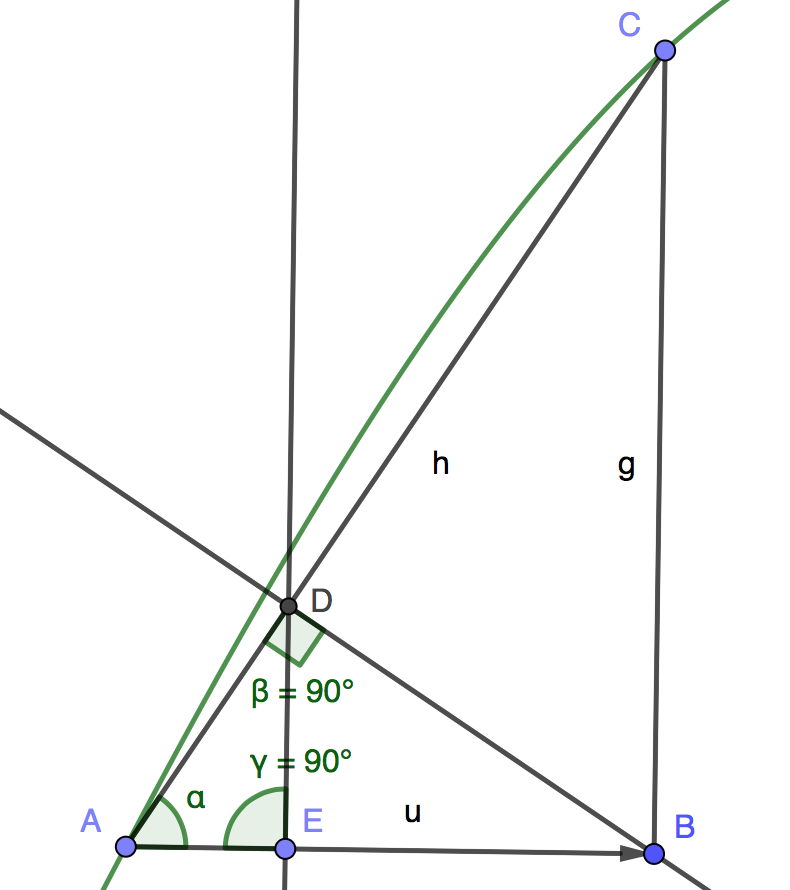
\includegraphics[width= 9cm, height = 9cm]{TRIANGOLO2.png}
	\caption{Parametric movement computations.}
	\label{fig:PMComputations}
\end{figure}

As already previously done, let's suppose that the starting point of our RL agent at epoch \textit{e} is the point \textit{A} with coordinates $(x, y)$. Because of the two dimensions, even in this case the agent can make only one of two actions for each epoch : \textit{move on} and \textit{go back}. Making a linear movement of the type \textit{move on} the arriving point at epoch \textit{e'} is \textit{B} with coordinates $(x', y)$. Knowing that the objective function is $f(x) = \sin(2x)$, we can now compute $f(x')$. We now know point \textit{C} with coordinates $(x', f(x'))$. \textit{u} is the {\tt movement amount} and \textit{CB} equals to $f(x') - f(x)$ is $\delta$. From trigonometry we know $\alpha$ but we are interested in knowing the real amount of movement done by the agent on the function or, at least, its approximation. We want to know how much is $\overline{AB}$.  From the first theorem of Euclid we know that \textit{in a right-angled triangle, the square constructed on a cathetus is equivalent to the rectangle that has for dimensions the hypotenuse and the projection of the cathetus on the hypotenuse}. This means that in a right-angled triangle, the cathetus is proportional medium between the hypotenuse and its own projection on it. According to this we can write the following proportion :

\begin{equation}
	i : u =  u : AD.
\end{equation}

So :

\begin{equation}
	AD = \dfrac{u * u}{i},
\end{equation}

that is the same of :

\begin{equation}
	 movementAmountApprox = \dfrac{{\tt movementAmount} * {\tt movementAmount}}{hypotenuse}
\end{equation}

of algorithm ~\ref{PMAlgo}.

The real question regards why select one method instead of the other one. The answer at this question is simple. Adopting the parametric approach the optimization process is longer but more accurate. In addition to this using the parametric approach we could ideally train our agent on a set of specific functions and it should do very good on a generic function using its knowledge about angles, actions and slope. 

Adopting the linear approach the optimization process is slower but less accurate. In addition to this using the linear approach we couldn't abstract from the concept of function.  This means that for every specific function we have to train our agent one more time.

\subsection{Implementation}

In order to formalize and solve our RL problem, we used the BURLAP (Brown-UMBC Reinforcement Learning and Planning) Java library developed and maintained by James MacGlashan. BURLAP uses a highly flexible system for defining states and and actions of nearly any kind of form, supporting discrete continuous, and relational domains. Planning and learning algorithms range from classic forward search planning to value function-based stochastic planning and learning algorithms.

In order to define specific MDPs, BURLAP offers a set of classes and interfaces (figure ~\ref{fig:UMLBurlap}).

\begin{figure} [h!]
	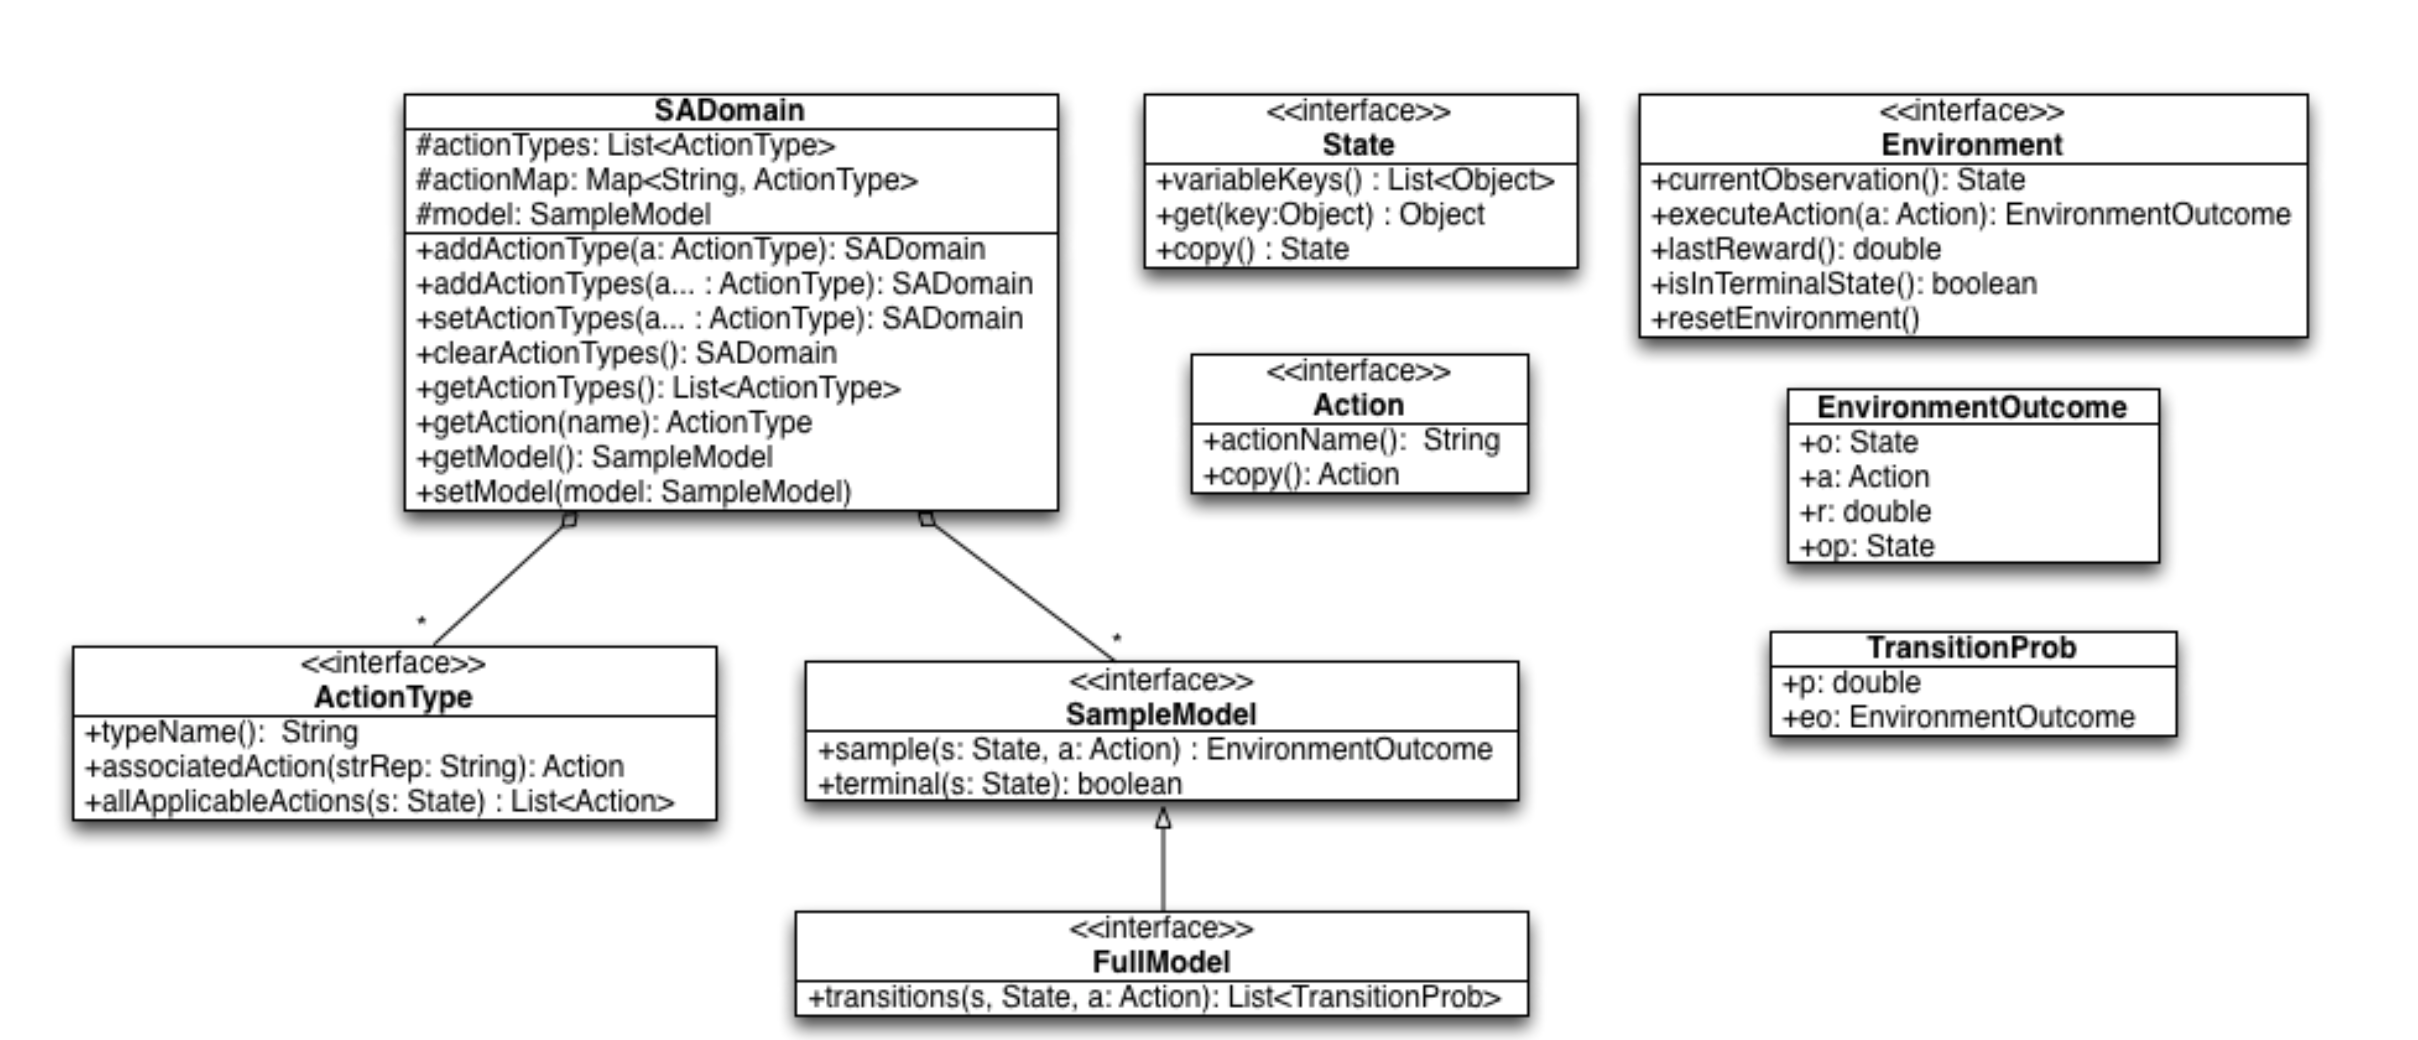
\includegraphics[width= 16cm, height = 9cm]{UMLBurlap.png}
	\caption{UML Digram of the Java interfaces/classes for an MDP definition.}
	\label{fig:UMLBurlap}
\end{figure}

A complete documentation for this framework can be find at (...). 

Starting from this features offered by BURLAP, we have extended interfaces and implemented abstract classes in order to modelling the problem described above as shown in figure (..). In our implementation ...

\begin{figure} [h!]
	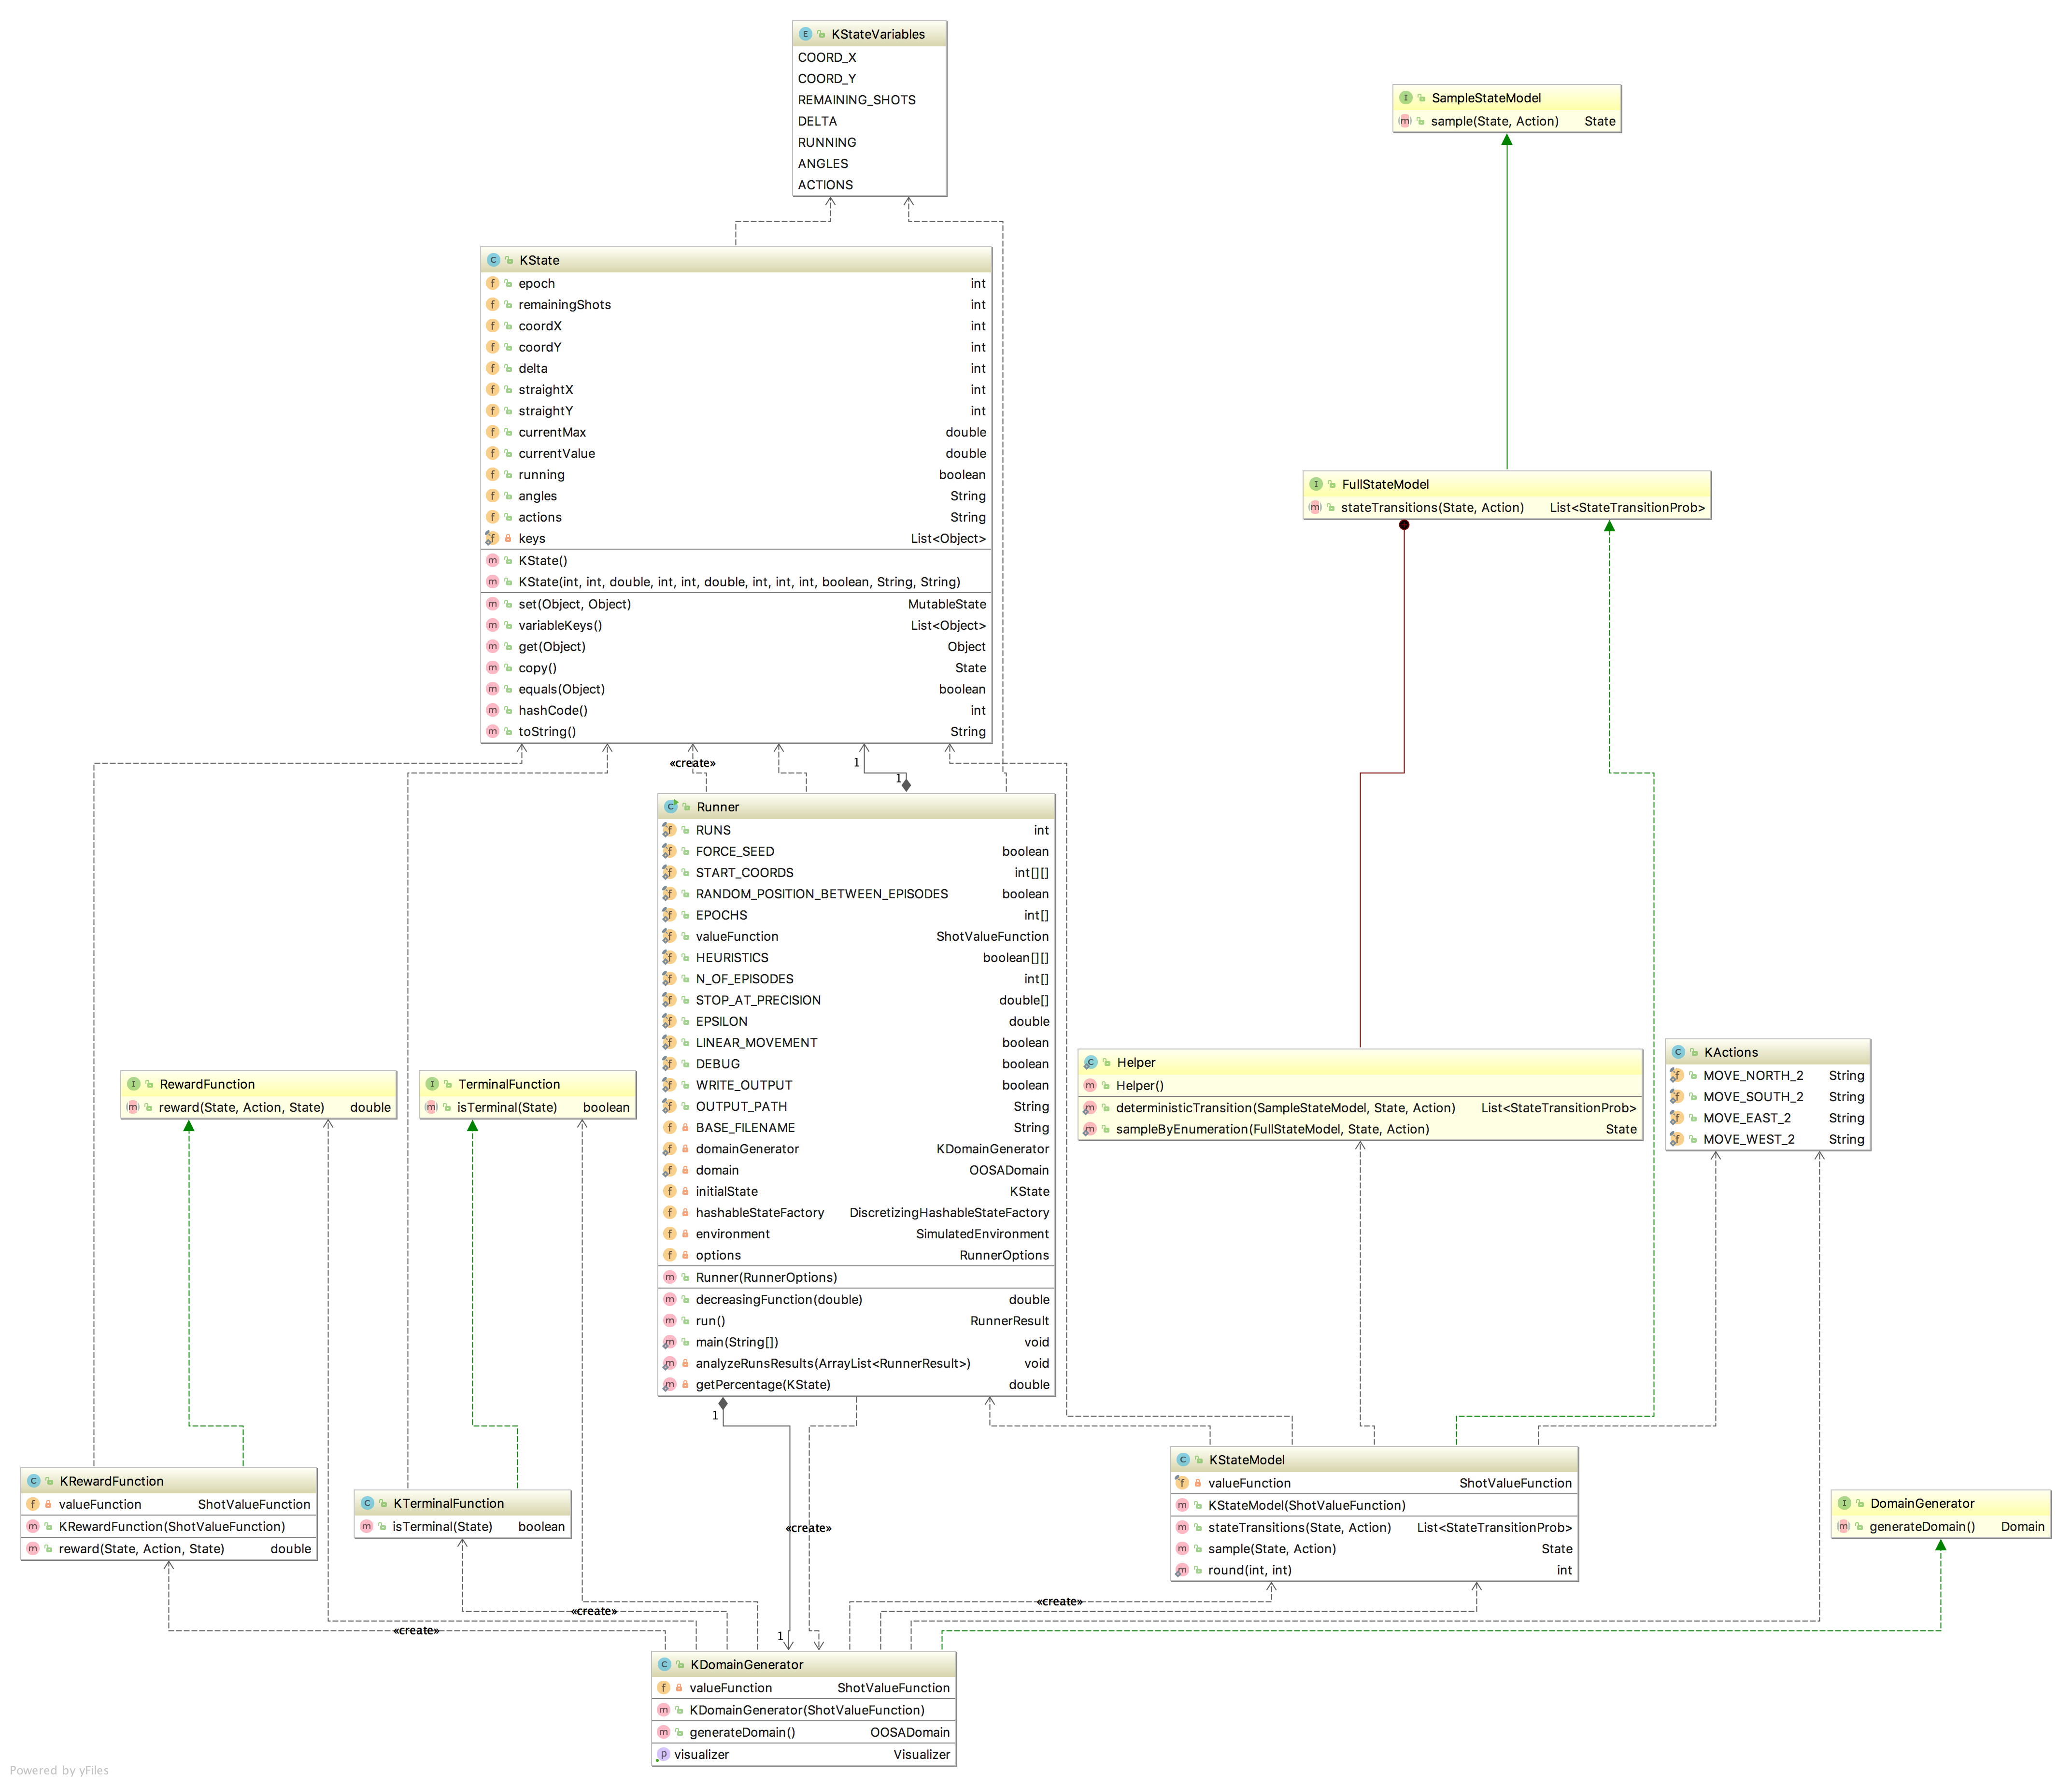
\includegraphics[width= 16cm, height = 18cm]{RLDiagram.png}
	\caption{Class diagram of RL black-box optimization tool.}
	\label{fig:RLDiagram}
\end{figure}
	\chapter{Experimental Setting}

The aim of this chapter is to describe the benchmarks of the experiments that have produced results analysed in the next few chapters. \\

In the first part of the chapter, the benchmark of the experiment conducted in order to analyse the performances of the innovative algorithm previously introduced, will be described. 

In the second part of the chapter, the benchmark of the experiment conducted on humans in order to better understand their acquisition functions in multivariate function learning, will be presented.

\section{Benchmark}

\subsection{Test Functions}

One of the experiments described in this work is about maximizing black-box functions adopting an RL based approach. A first relevant choice is about selecting suitable \textit{test functions}. In applied mathematics, test functions, also known as \textit{artificial landscapes}, are useful to evaluate characteristics of optimization algorithms. Four test functions have been chosen for this purpose :

\begin{itemize}
	\item Himmelblau' s Function;
	\item Sphere Function;
	\item Beale Function;
	\item Styblinski-Tang' s Revised Function.	
\end{itemize}

\subparagraph{Himmelblau' s Function} In mathematical optimization, Himmelblau' s function is a continuous, bivariate, multi-modal function. The original function is defined by: 

\begin{equation}
	f(x, y) = (x^2 + y -11)^2 + (x + y^2 - 7)^2
\end{equation}

It has four local minima :

\begin{itemize}
	\item $f(3.0, 2.0) = 0.0$;
	\item $f(-2.805118, 3.131312) = 0.0$;
	\item $f(-3.779310, -3.283186) = 0.0$;
	\item $f(3.584428, -1848126) = 0.0$.
\end{itemize}
	
The function can be defined on any input domain but it is usually evaluated on $x \in [-5, 5]$ and $y \in [-5, 5]$.

\begin{figure}[h!]
	\centering
	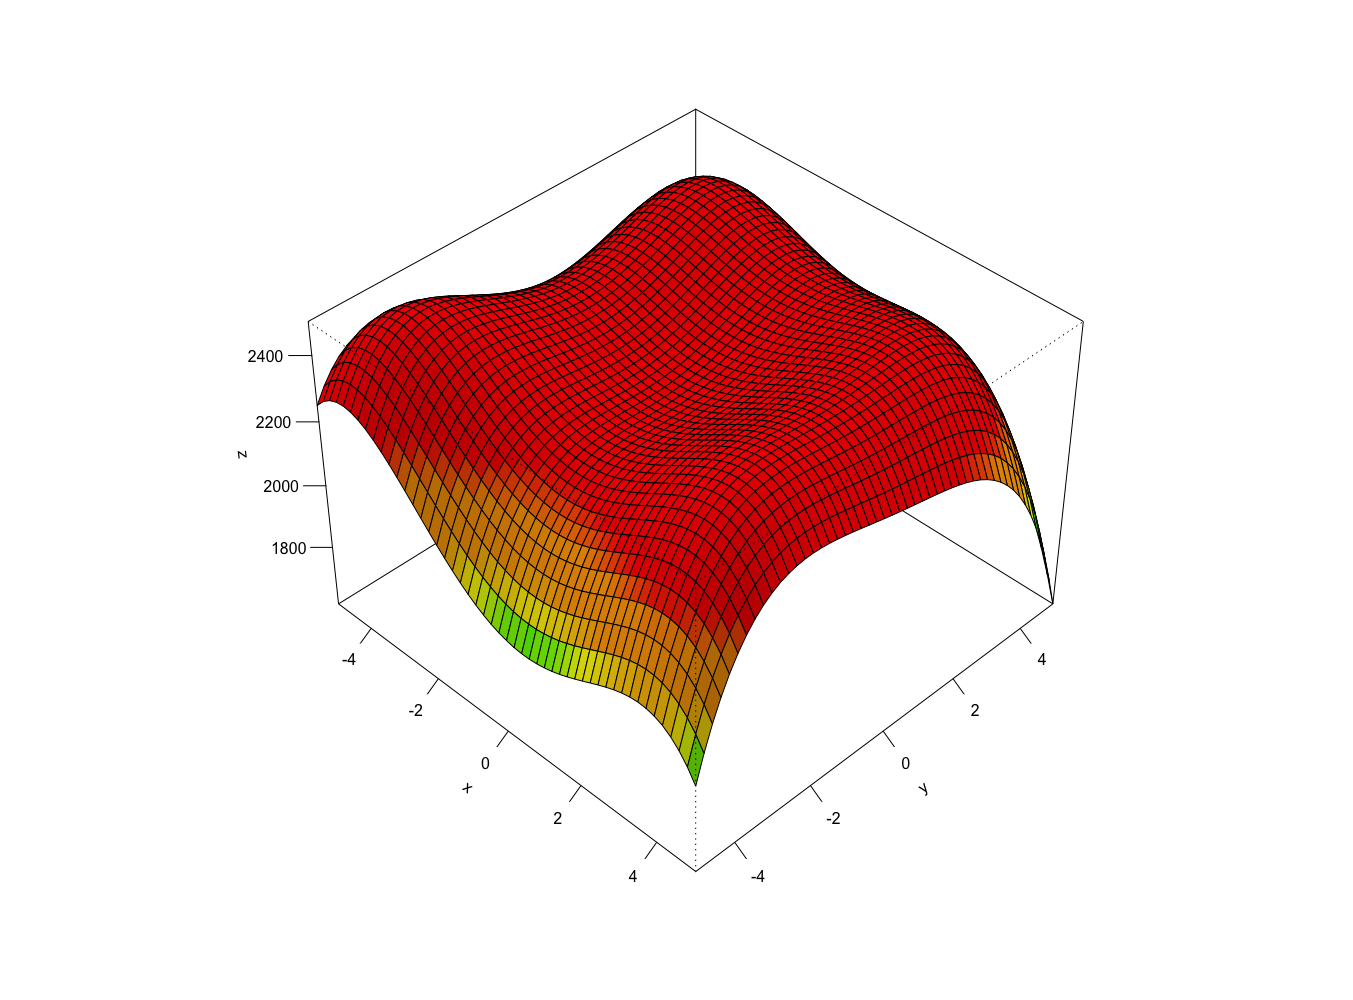
\includegraphics[width= 8cm, height = 8cm]{modifiedHimmelblau.png}
	\caption{Customized Himmelblau' s Function.}
	\label{fig:CustomizedHimmelblauFunction}
\end{figure}

Because of the aim to maximize the function has been inverted as follow :

\begin{equation}
f(x, y) = -(x^2 + y -11)^2 + (x + y^2 - 7)^2
\end{equation}

It has been picked up of $2500$ units in order to have as less as possible negative values. So the final adopted function is :
 
\begin{equation}
f(x, y) = -(x^2 + y -11)^2 + (x + y^2 - 7)^2 + 2500
\end{equation}

This function has its global maximum in $f(x, y) = 2500$. 

In order to represent this customized version of Himmelblau' s Function using Java Graphical Environment, it has been mapped in a space of $600 \times 600$ pixels and it has been properly rotated. The resulting contour plot is the one represented in figure ~\ref{fig:ContourPlotCustomizedHimmelblauFunction}. \\

\begin{figure}[h!]
	\centering
	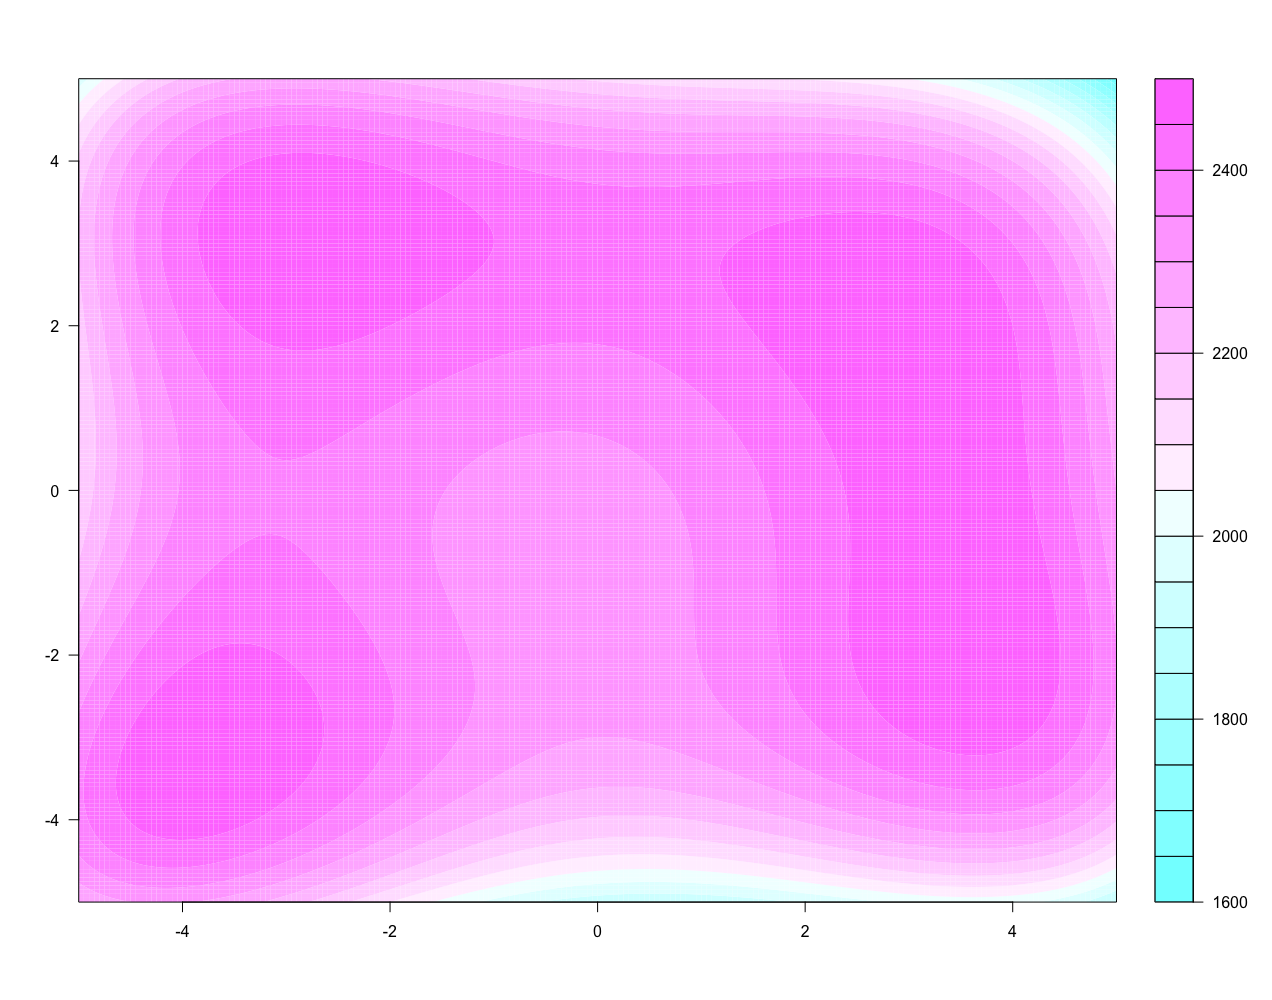
\includegraphics[width= 4cm, height = 4cm]{himmelblau.png}
	\caption{Contour plot of customized version of Himmelblau' s Function.}
	\label{fig:ContourPlotCustomizedHimmelblauFunction}
\end{figure}
 
\subparagraph{Sphere Function} In mathematical optimization, Sphere function is a continuous, bivariate, uni-modal function. \\

The original function is defined by: 

\begin{equation}
f(x, y) = (x^2 + y^2) 
\end{equation}

It has a global minimum in $f(x, y) = 0$.

The function can be defined on any input domain but it is usually evaluated on $x \in [-10, 10]$ and $y \in [-10, 10]$. 

\begin{figure}[h!]
	\centering
	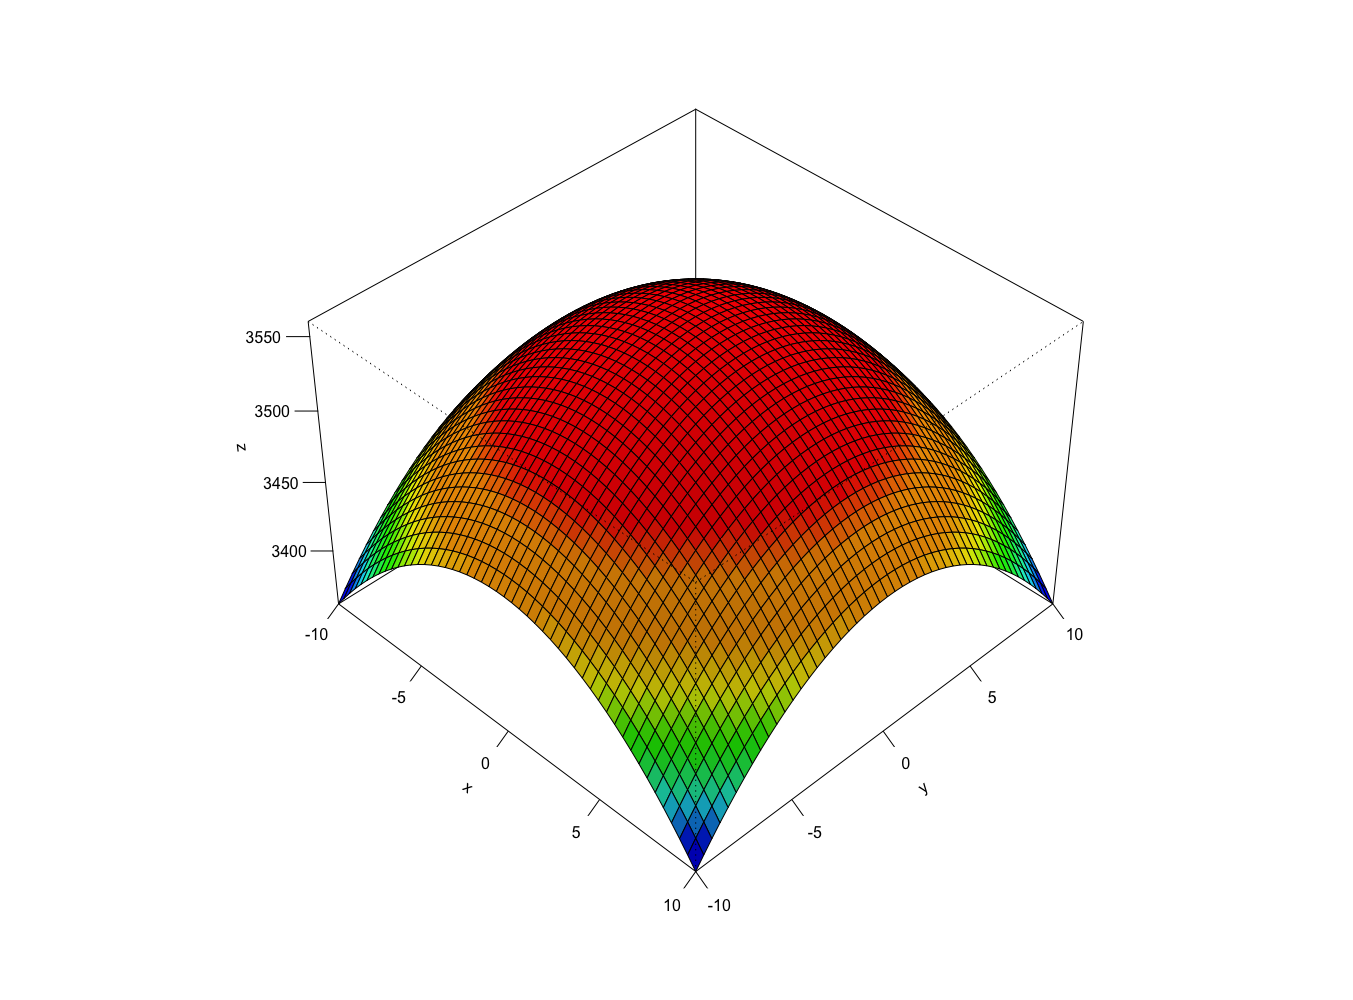
\includegraphics[width= 8cm, height = 8cm]{customizedParaboloid.png}
	\caption{Customized Sphere Function.}
	\label{fig:CustomizedParaboloidOfRevolution}
\end{figure}

Because of the aim to maximize, the function has been inverted as follow :

\begin{equation}
f(x, y) = -(x^2 + y^2)
\end{equation}

and it has been picked up of $3560$ units in order to have as less as possible negative values. So the final adopted function is :

\begin{equation}
f(x, y) = -(x^2 + y^2) + 3560
\end{equation}

This function has its local maximum in $f(x, y) = 3560$.

In order to represent this customized version of Sphere function function using Java Graphical Environment, it has been mapped in a space of $600 \times 600$ pixels and it has been properly rotated. The resulting contour plot is the one represented in figure ~\ref{fig:ContourPlotCustomizedParabolicFunction} 

\begin{figure}[h!]
	\centering
	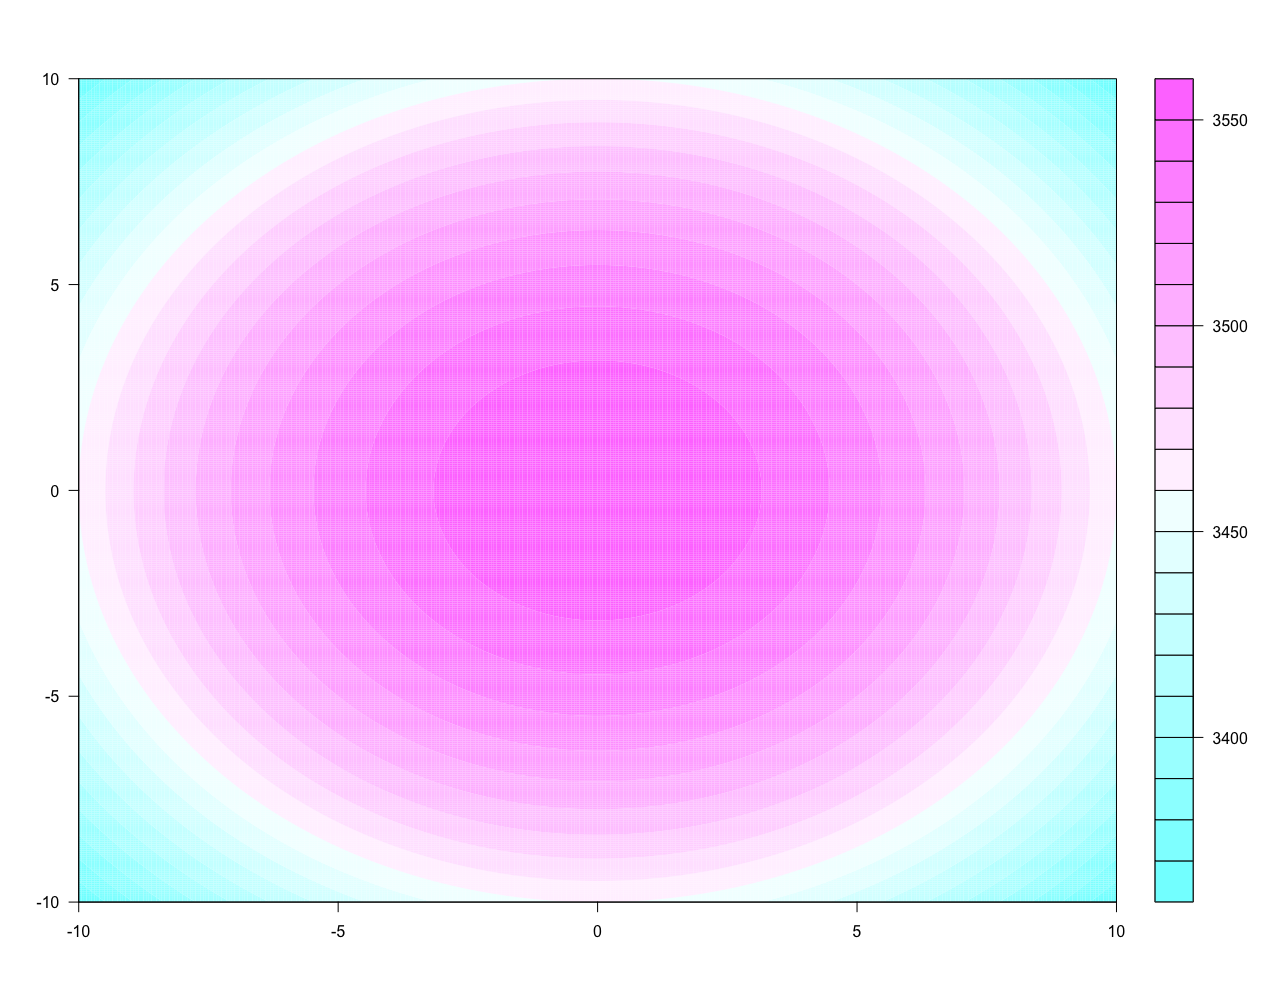
\includegraphics[width= 4cm, height = 4cm]{parabolic.png}
	\caption{Contour plot of customized Sphere Function.}
	\label{fig:ContourPlotCustomizedParabolicFunction}
\end{figure}

\subparagraph{Beale Function} In mathematical optimization, Beale Function is a continuous, bivariate, multi-modal function. The original function is defined by: 

\begin{equation}
f(x, y) = (1.5 - x + xy)^2 + (2.25 - x + xy^2)^2 + (2.625 - x + xy^3)^2
\end{equation}

The function can be defined on any input domain but it is usually evaluated on $x \in [-3, 3]$ and $y \in [-3, 3]$. \\

It has one global minimum in: $f(x, y) = 0$. 

Because of the aim to maximize, it has been inverted as follow:

\begin{equation}
f(x, y) = -((1.5 - x + xy)^2 + (2.25 - x + xy^2)^2 + (2.625 - x + xy^3)^2)
\end{equation}

\begin{figure}[h!]
	\centering
	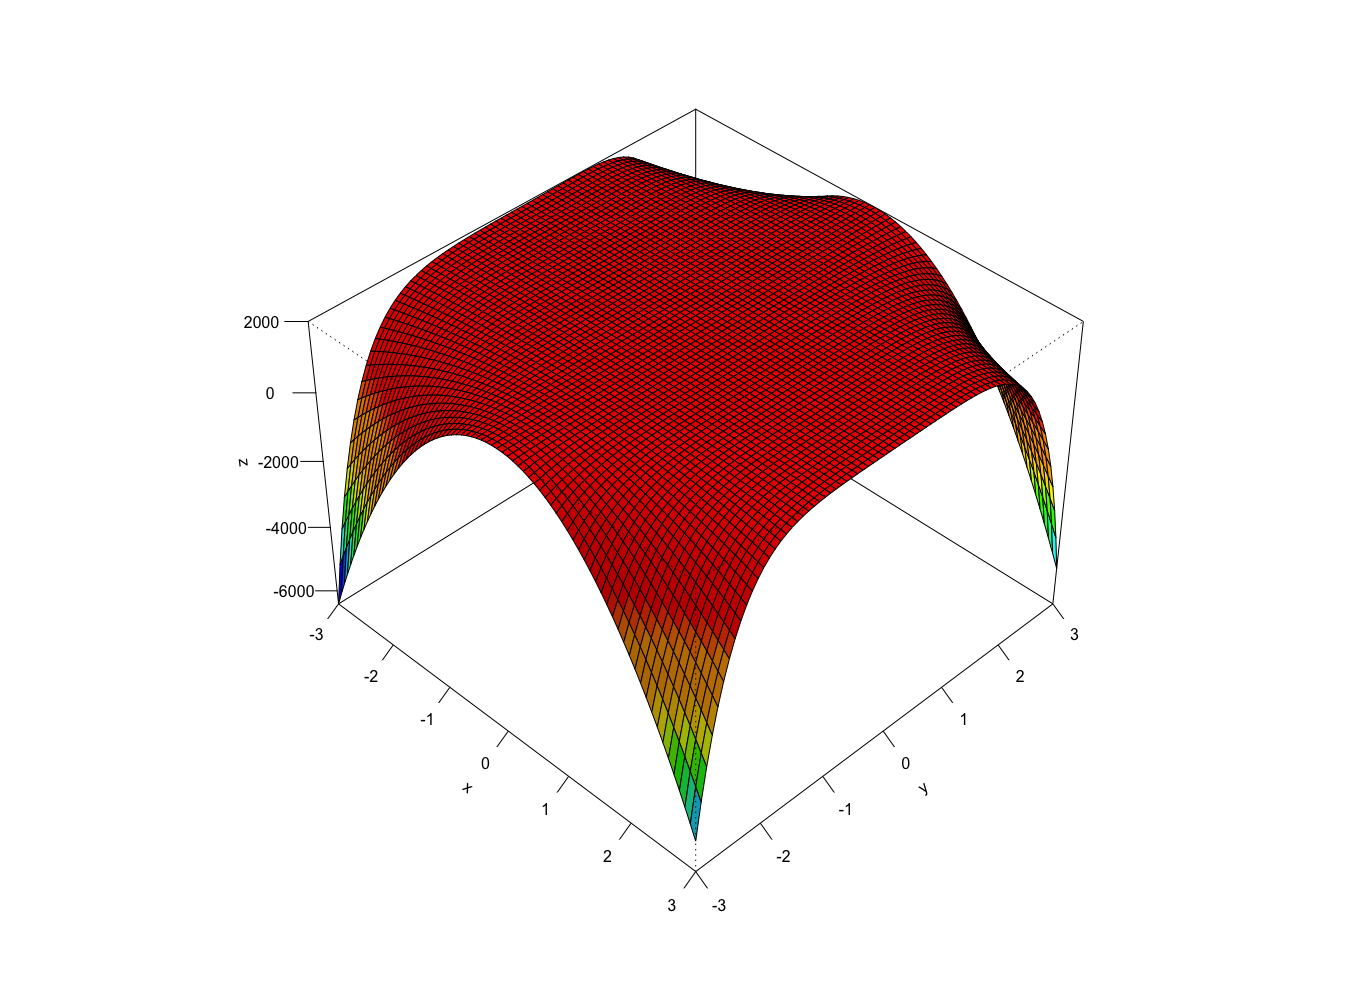
\includegraphics[width= 8cm, height = 8cm]{customizedBeale.png}
	\caption{Customized Beale Function.}
	\label{fig:CustomizedBealeFunction}
\end{figure}

It has been picked up of $2000$ units in order to have as less as possible negative values. So the final adopted function is :

\begin{equation}
f(x, y) = -((1.5 - x + xy)^2 + (2.25 - x + xy^2)^2 + (2.625 - x + xy^3)^2) + 2000
\end{equation}

This customized function has its global maximum in $f(x, y) = 2000$.

In order to represent this function using Java Graphical Environment it has been mapped in a space of $600 \times 600$ pixels and it has been properly rotated. The resulting contour plot is the one represented in figure ~\ref{fig:ContourPlotCustomizedBealeFunction} 

\begin{figure}[h!]
	\centering
	
\includegraphics[width= 4cm, height = 4cm]{beale.png}
	\caption{Contour plot of customized Beale Function.}
	\label{fig:ContourPlotCustomizedBealeFunction}
\end{figure}

\subparagraph{Styblinski-Tang Revised Function} In mathematical optimization, Styblinski-Tang' s Function is a continuous, bivariate function. The original function is defined by :

\begin{equation}
	f(x) = \dfrac{\sum_{i=1}^{n} x_{i}^4 -16x_{i}^2 +5x_{i}}{2}
\end{equation}

\begin{figure}[h!]
	\centering
	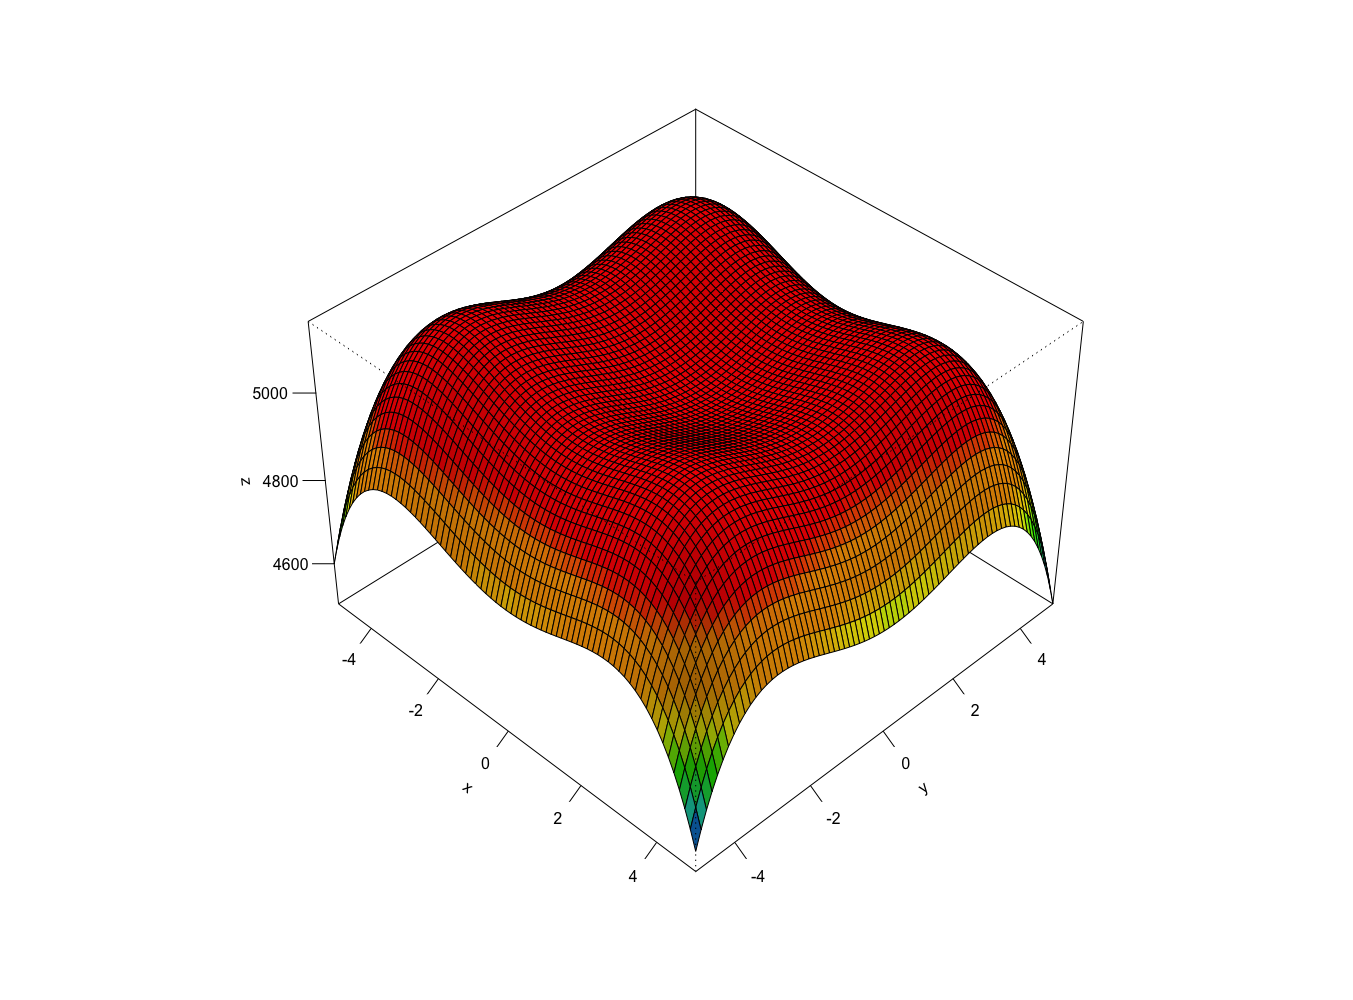
\includegraphics[width= 8cm, height = 8cm]{customizedStyblinski.png}
	\caption{Customized Styblinski Function.}
	\label{fig:CustomizedStyblinskiFunction}
\end{figure}

In this thesis the bivariate version of the original function multiplied by two in order to make it less flatten, is considered:

\begin{equation}
f(x, y) = (x^4 - 16x^2 + 5x) + (y^4 - 16y^2 + 5y).
\end{equation}

The function can be defined on any input domain but it is usually evaluated on $x \in [-5, 5]$ and $y \in [-5, 5]$. \\

Because of the aim to maximize, it has been inverted as follow :

\begin{equation}
f(x, y) = -((x^4 - 16 * x^2 + 5 * x) + (y^4 - 16 * y^2 + 5 * y))
\end{equation}

It has been picked up of $5000$ units in order to have as less as possible negative values. So the final adopted function is: 

\begin{equation}
f(x, y) = -((x^4 - 16 * x^2 + 5 * x) + (y^4 - 16 * y^2 + 5 * y)) + 5000
\end{equation}

This customized function has its global maximum in $f(x, y) = 5156.6638$. In order to represent this function using Java Graphical Environment it has been mapped in a space of $600 \times 600$ pixels and it has been properly rotated. The resulting contour plot is the one represented in figure ~\ref{fig:ContourStyblinskiFunction}.

\begin{figure}[h!]
	\centering
	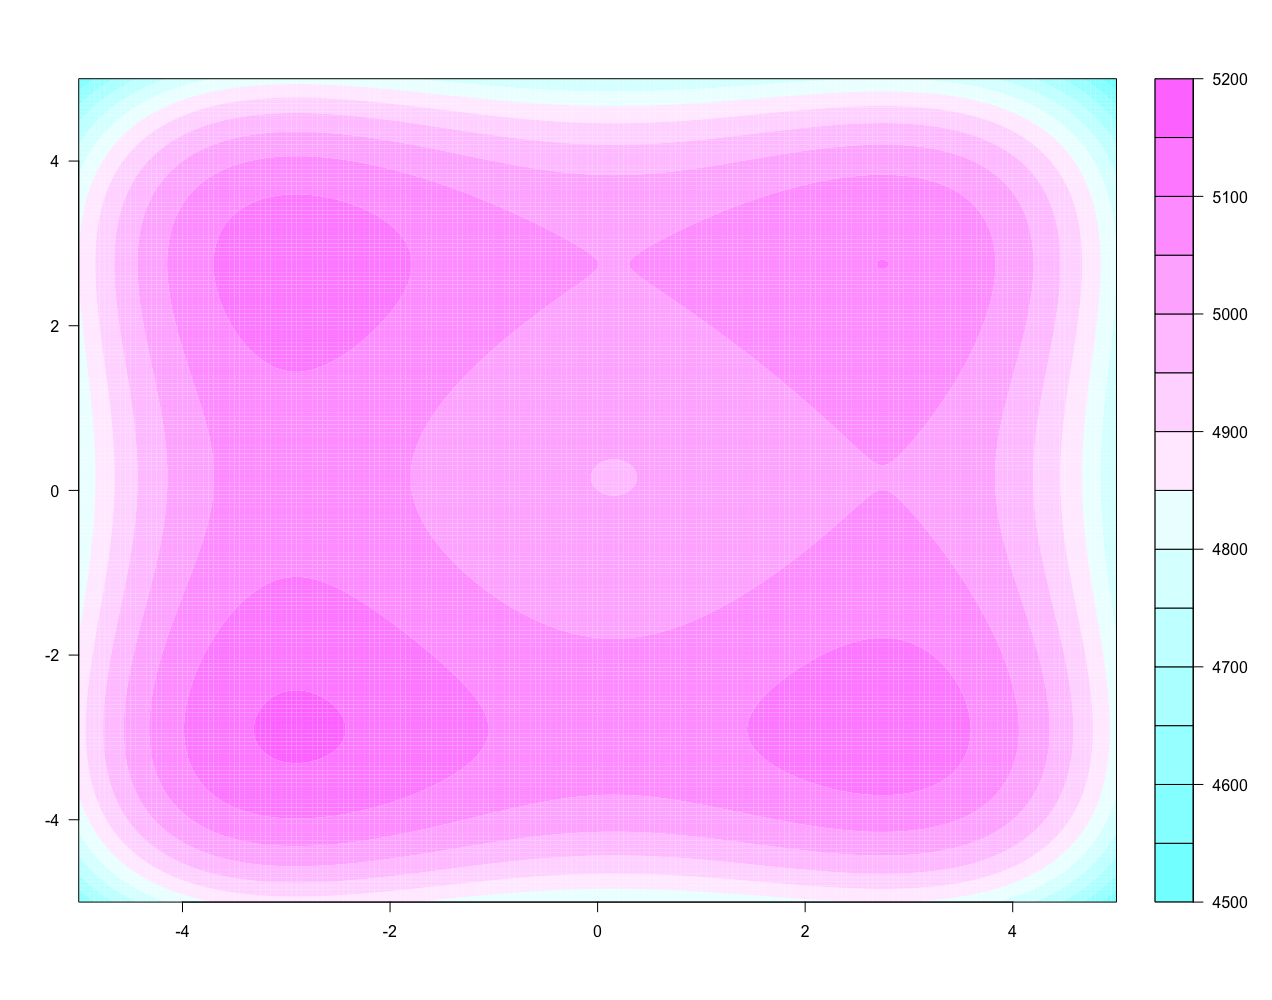
\includegraphics[width= 4cm, height = 4cm]{styblinski.png}
	\caption{Contour plot of customized Styblinski Function.}
	\label{fig:ContourStyblinskiFunction}
\end{figure}

\begin{sidewaystable} 
	\centering
	\caption{Objective Functions'  Summary Table}
	\begin{tabular}
		{l l l l l} \hline Name & Formula & Domain & Optimal \textit{f} & Sketch \\
		\hline Himmelblau & \vtop{\hbox{\strut $f(x, y) = - ((x^2 + y -11)^2+$}\hbox{\strut $+(x + y^2 - 7)^2) + 2500$}} & $x, y \in [-5;+5]$ & $2500$ & \parbox[c]{1em}{
			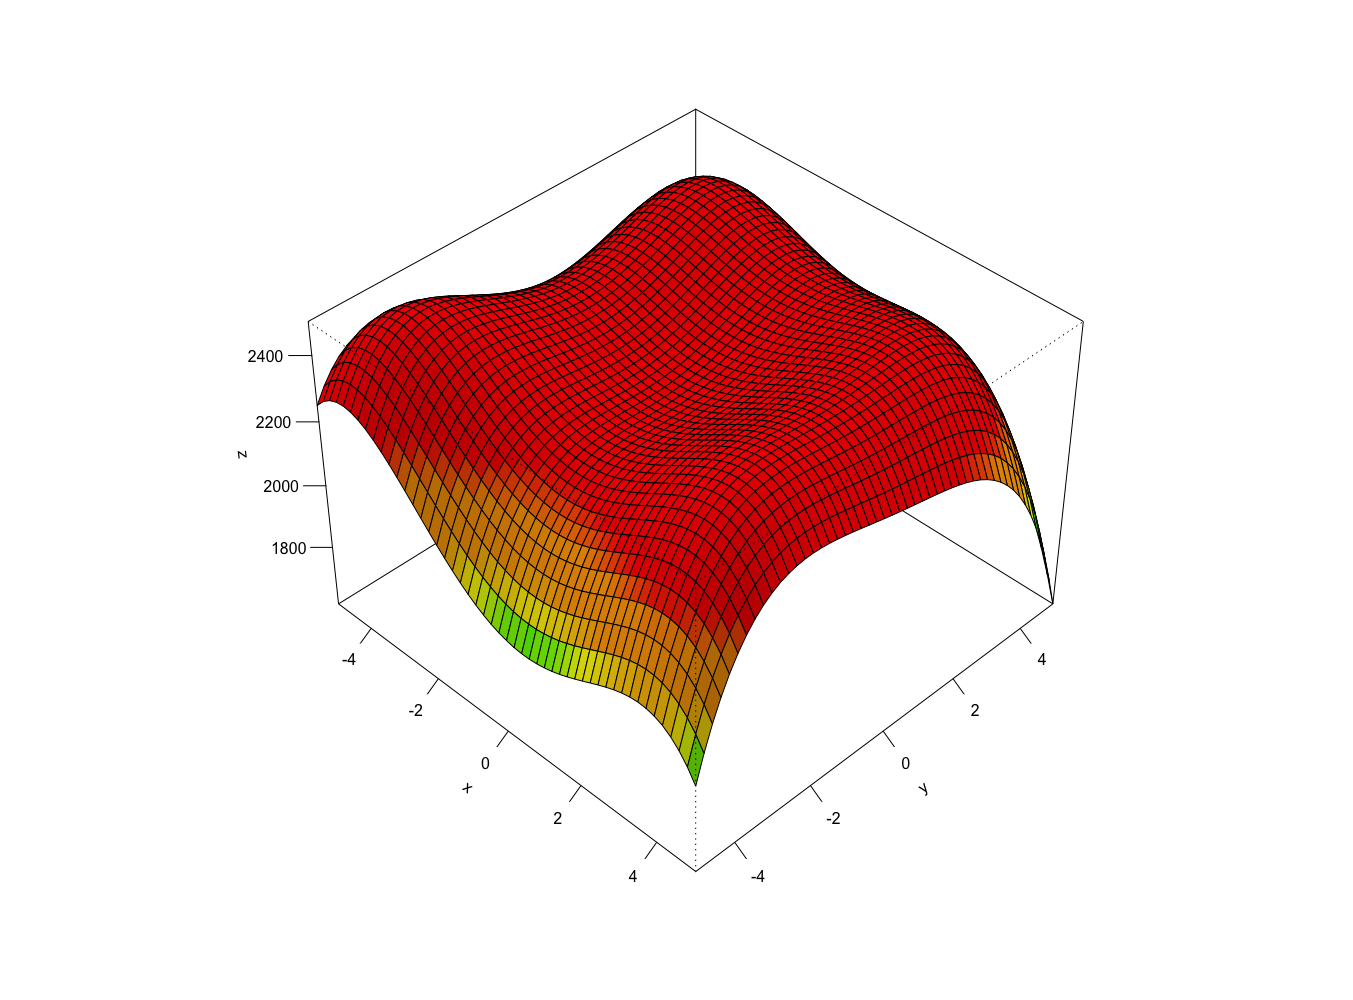
\includegraphics[width=1.7in]{modifiedHimmelblau}} \\
		Sphere & $f(x, y) = -(x^2 + y^2) + 3560$ &$x, y \in [-10;+10]$ & $3560$ & \parbox[c]{1em}{
			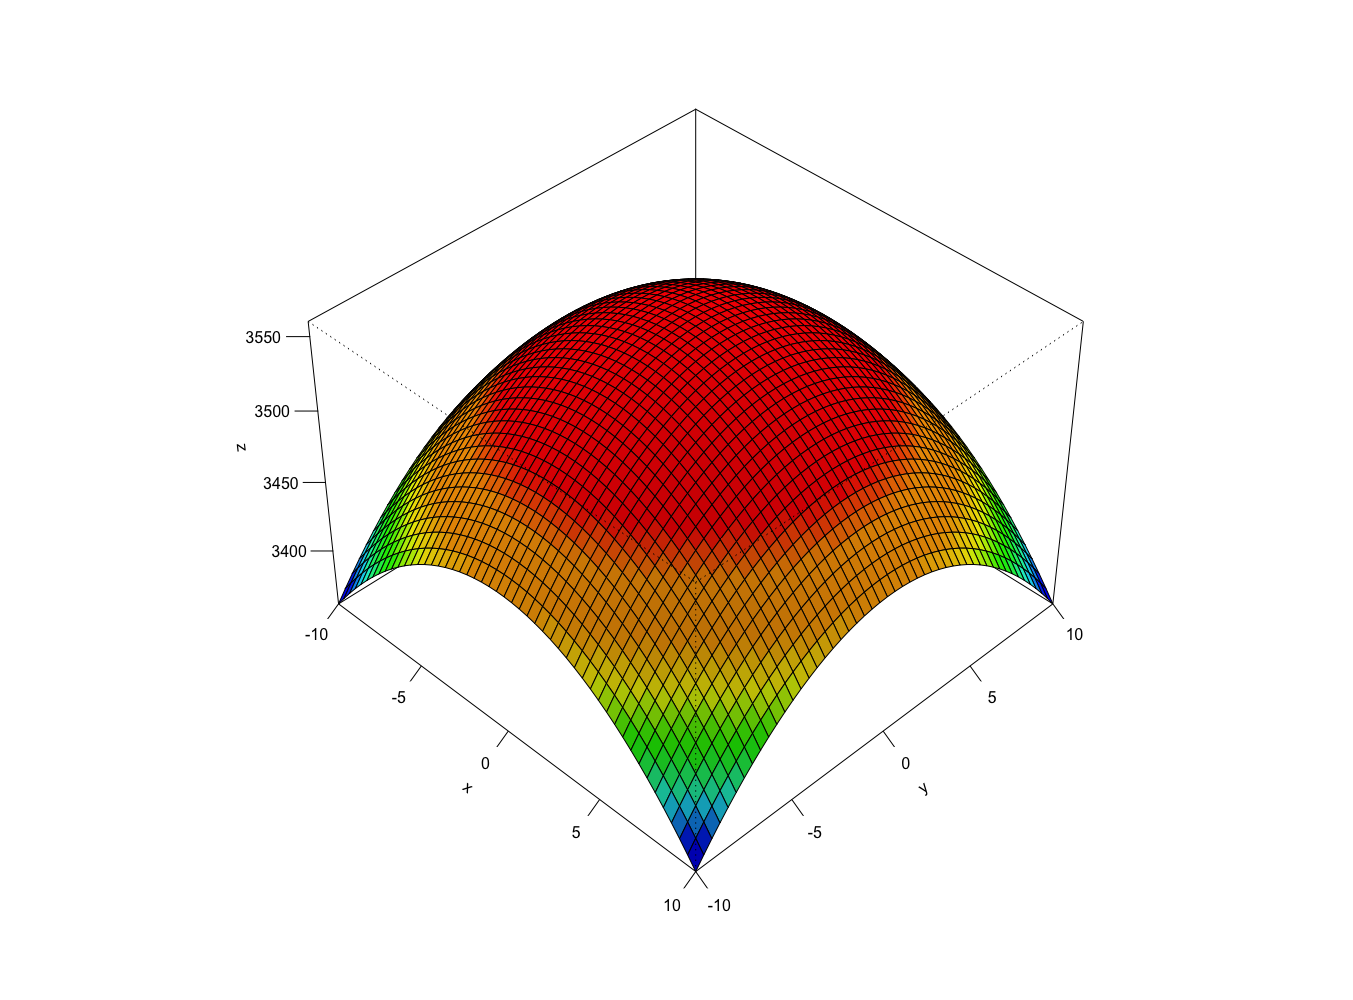
\includegraphics[width=1.7in]{customizedParaboloid}} \\
		Beale & \vtop{\hbox{\strut $f(x, y) = - ((1.5 - x + xy)^2 + ) $}\hbox{\strut $+ (2.25-x+xy^2)^2 + $}\hbox{\strut $+ (2.625 -x+xy^3)^2) + 2000 $}} &$x, y \in [-3;3]$ & $2000$ & \parbox[c]{1em}{
			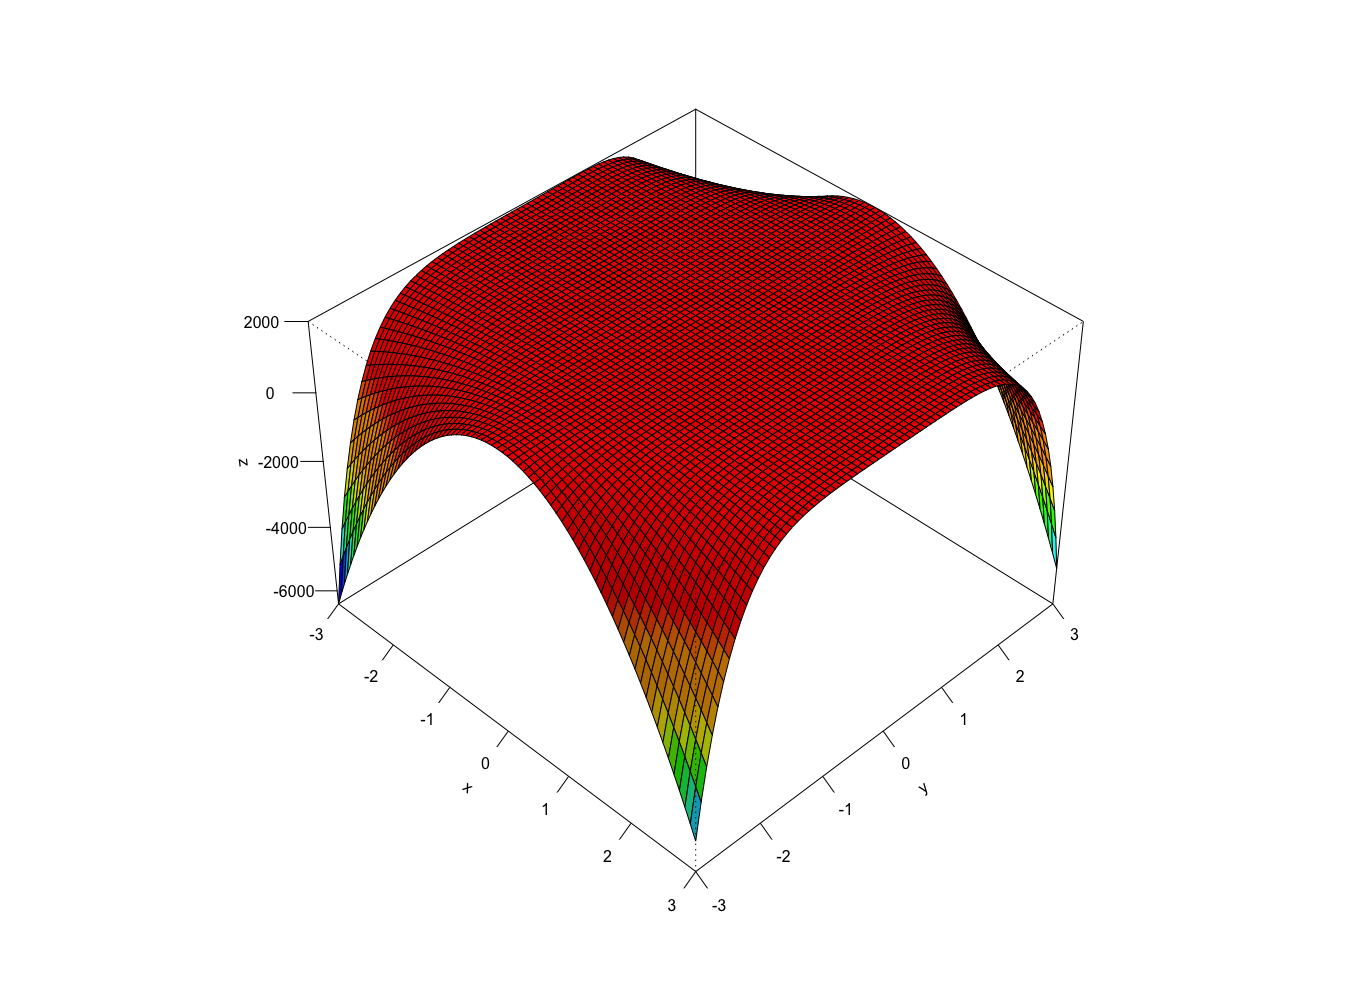
\includegraphics[width=1.7in]{customizedBeale}} \\
		Styblinski-Tang & \vtop{\hbox{\strut $f(x, y) = -((x^4 - 16 * x^2 + 5 * x) + $}\hbox{\strut $(y^4 - 16 * y^2 + 5 * y)) + 5000$}} &$x, y \in [-5;+5]$ & $5156.6638$ & \parbox[c]{1em}{
			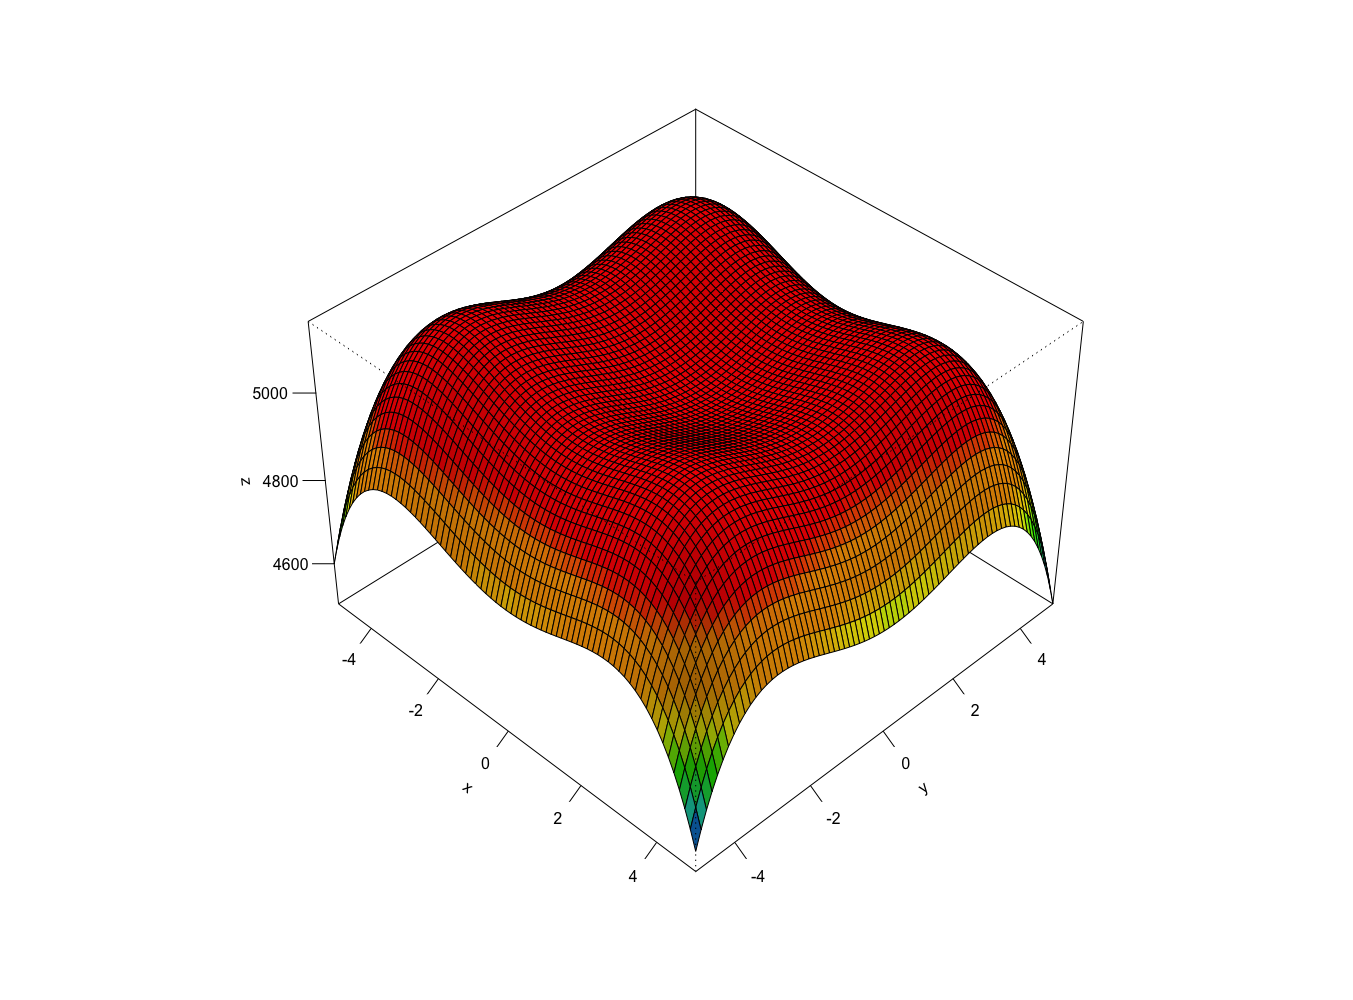
\includegraphics[width=1.7in]{customizedStyblinski}} \\
		\hline
	\end{tabular}
\end{sidewaystable}

\subsection{Basic SARSA($\lambda$) Algorithm' s Configuration} The RL algorithm employed in the current work is the {\tt SARSA($\lambda$)} one. It has only one configuration (summarized in table ~\ref{ConfigurationTable}) and four different declinations (summarized in table ~\ref{DeclinationTable}).

\begin{table} [h!]
	\centering
	\resizebox{\linewidth}{!} {	
	\begin{tabular}{|c||c|c|c|c|c|c|c|}
		\hline 
		& \textbf{$\lambda$}  & \textbf{$\epsilon$} & \textbf{qInit} & \textbf{Learning Rate} & \textbf{Discount Factor}  & \textbf{Episodes}  & \textbf{Epochs} \\
		\hline \hline Configuration $1$
		& $0.1$ & $0.1$ & $0$ & $1$ & $0.99$  & $150$ & $101$  \\ 
		\hline
	\end{tabular}
}
\caption{Configuration Table}
\label{ConfigurationTable}
\end{table}

\begin{table} [h!]
	\centering	
	\begin{tabular}{|c||c|}
		\hline \textbf{Declination}
		& \textbf{Type of search} \\ 
		\hline \hline Declination 1
		&  Linear, not random search\\ 
		\hline Declination 2
		& Linear, random search \\ 
		\hline Declination 3
		& Parametric, not random search \\ 
		\hline Declination 4
		&  Parametric, random search\\ 
		\hline 
	\end{tabular} 
\caption{Declination table}
\label{DeclinationTable}
\end{table}

In the proposed configuration a low $\lambda$ value is employed. Typically it should be used lower learning rate when a higher value of $\lambda$ is employed. However, in this case, it has been decided to use the highest possible learning rate. The logical consequence to this choice is to decrease the $\lambda$ value. \\

An $\epsilon$ value equals to $0.1$ means that $90\%$ of selected actions depends on the history, whereas the remaining $10\%$ represents a random choice having absolutely no relations with the previous history. \\ 

A discount factor set to $0.99$ means the rewards will propagate as long as possible through time. \\

Assuming that each epoch's action has an high cost, the number of epochs must be as low as possible assuring, at the same time, a reasonable training space. In order to satisfy these requirements, the number of episodes is set to $150$. Each episode is composed by $101$ epochs. The choice about those two parameters depends on results of specific tests conducted in order to understand correct values to employ. \\

Note that in addition to the $150$ training episodes there is also a greedy one. In this last episode the $\epsilon$ value and the \textit{learning rate} parameter are set to $0$. Instead, the number of epochs, the {\tt qInit} parameter and the discount factor are left unchanged.  \\

Each declination of {\tt SARSA(\textit{$\lambda$})} is linear or parametric (search techniques described in the previous chapter). In addition to this each declination could be simple or random. In the last case the starting point for each episode is randomly selected from a set of ($600 \times 600$) possibilities. In the implementation of random search, the BURLAP {\tt RandomFactory} class has been used. {\tt RandomFactory} allows to logically group various random generators. The {\tt id} is set to $0$ and the {\tt seed} is set to $1$.

\section{Experiment on Humans}

The test conducted on humans affects a cross-section of twenty-three people. In the selection process of test subjects the following three parameters with corresponding bounds were considered :

\begin{itemize}
	\item \textbf{Sex} $\in \{Male, Female\}$
	\item \textbf{Age} $\in [19, 50]$
	\item \textbf{Math Knowledge Level} $\in \{Elementary, Medium, High\}$ 
\end{itemize} 

$71\%$ of test subjects are males, the remaining $29\%$ are females (plot (a) of figure \ref{fig:testSubjectsAttributes}). \\

$75\%$ of test subjects has an age between $19$ and $22$. The $21\%$ of test subjects has an age between $23$ and $26$. The remaining $4\%$ of test subjects has an age $> 26$ (plot (c) of figure \ref{fig:testSubjectsAttributes}). \\

The mathematical knowledge level is considered elementary if the subject has never attended a course of basic calculus. The mathematical knowledge level is considered medium if the subject has attended at least a basic calculus course. The mathematical knowledge level is considered high if the subject has attended an advanced calculus course. \\

$52\%$ of test subjects has an high mathematical educational level. The $43\%$ of test subjects has a medium mathematical educational level. The remaining $4\%$ of test subjects has an elementary, mathematical education level (pot (b) of figure \ref{fig:testSubjectsAttributes}). \\

\begin{figure}[h!]
	\begin{center}
		\subfigure[]{%
			\label{fig:sex}
			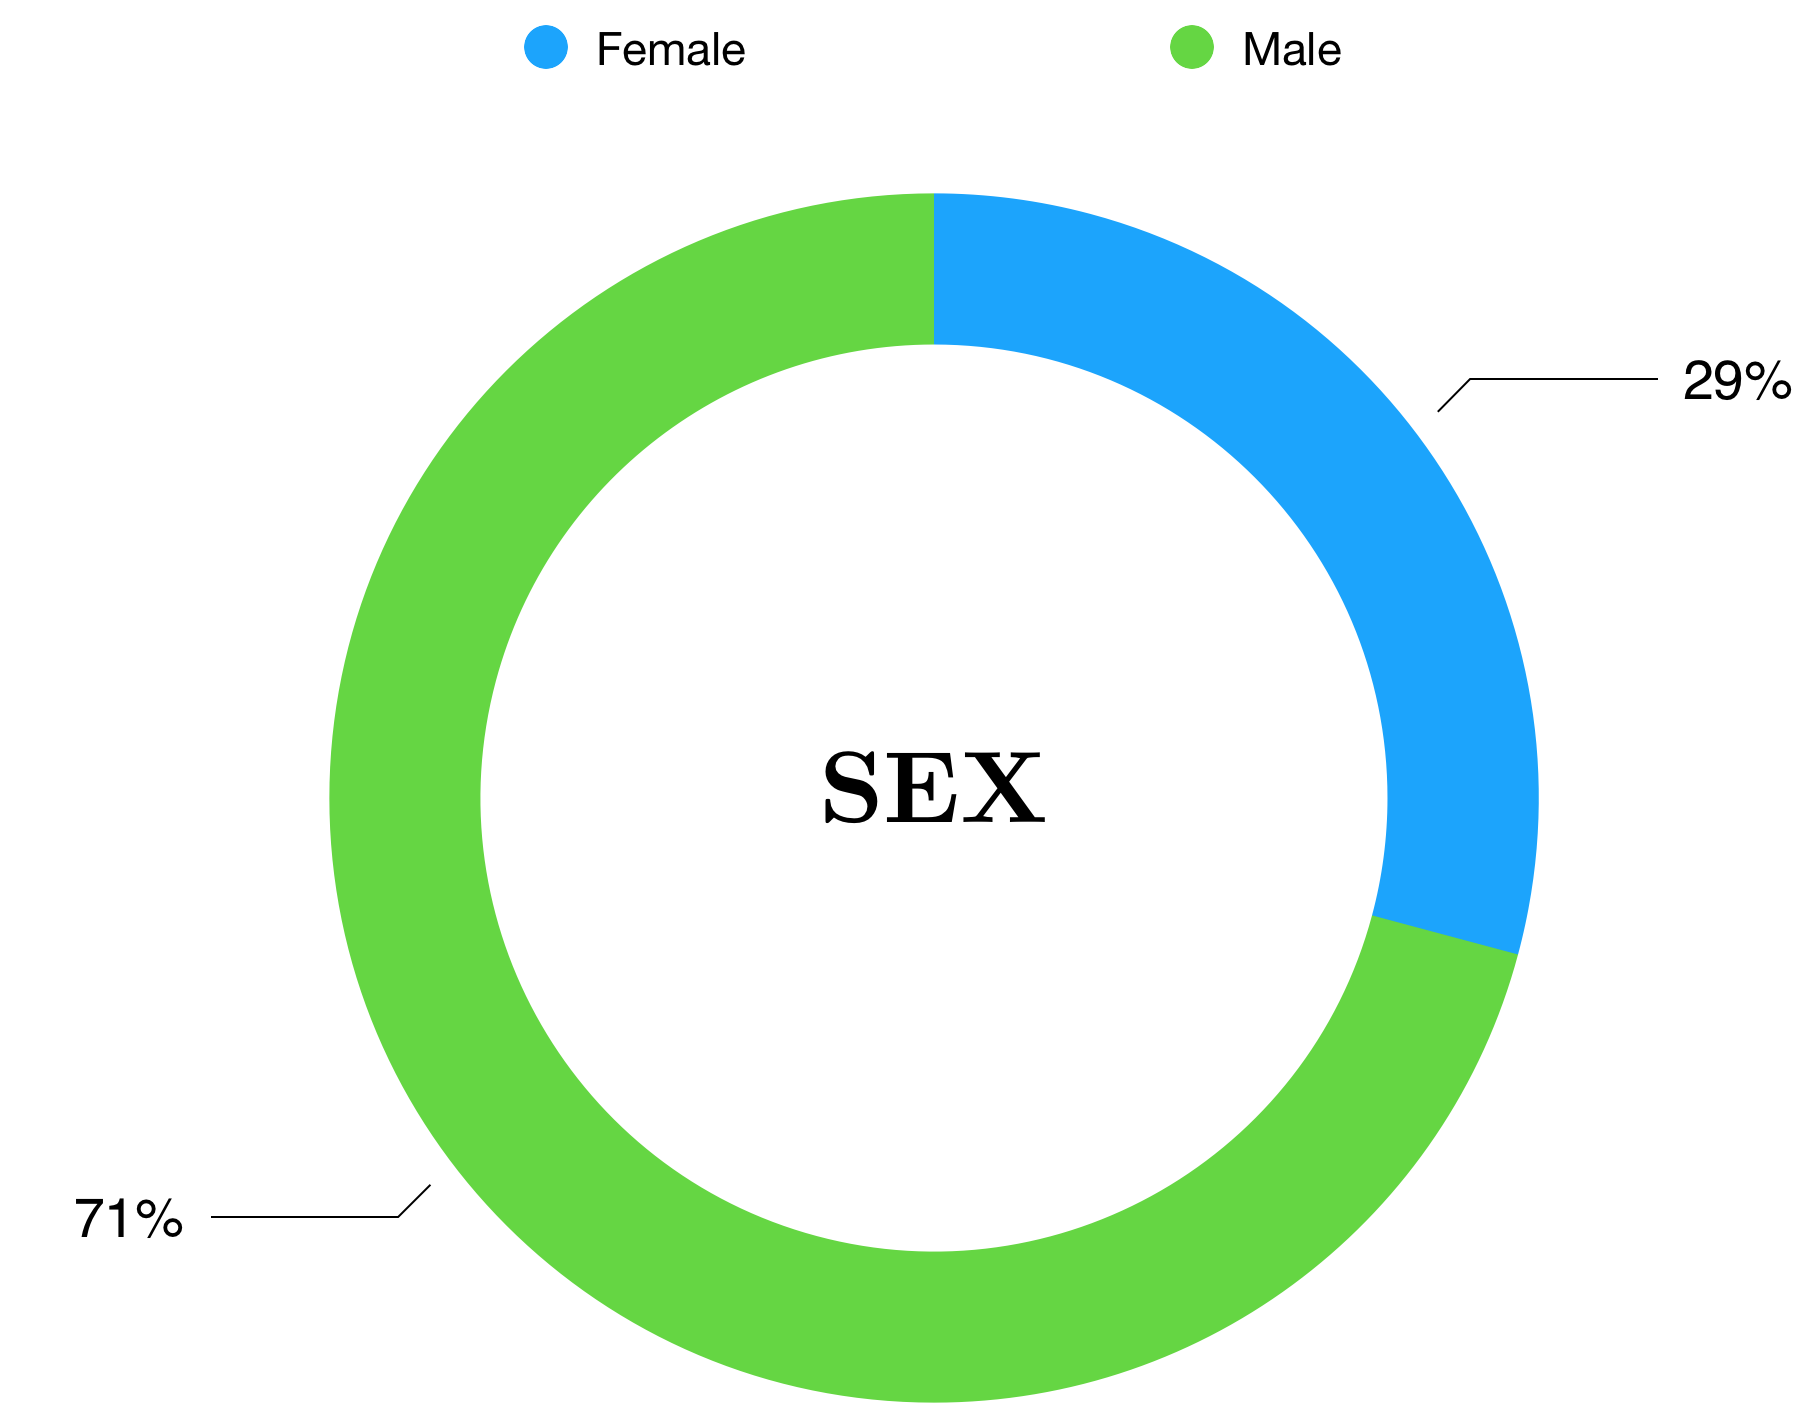
\includegraphics[width=0.4\textwidth]{Sex}
		}
		\subfigure[]{%
			\label{fig:mathEdLevel}
			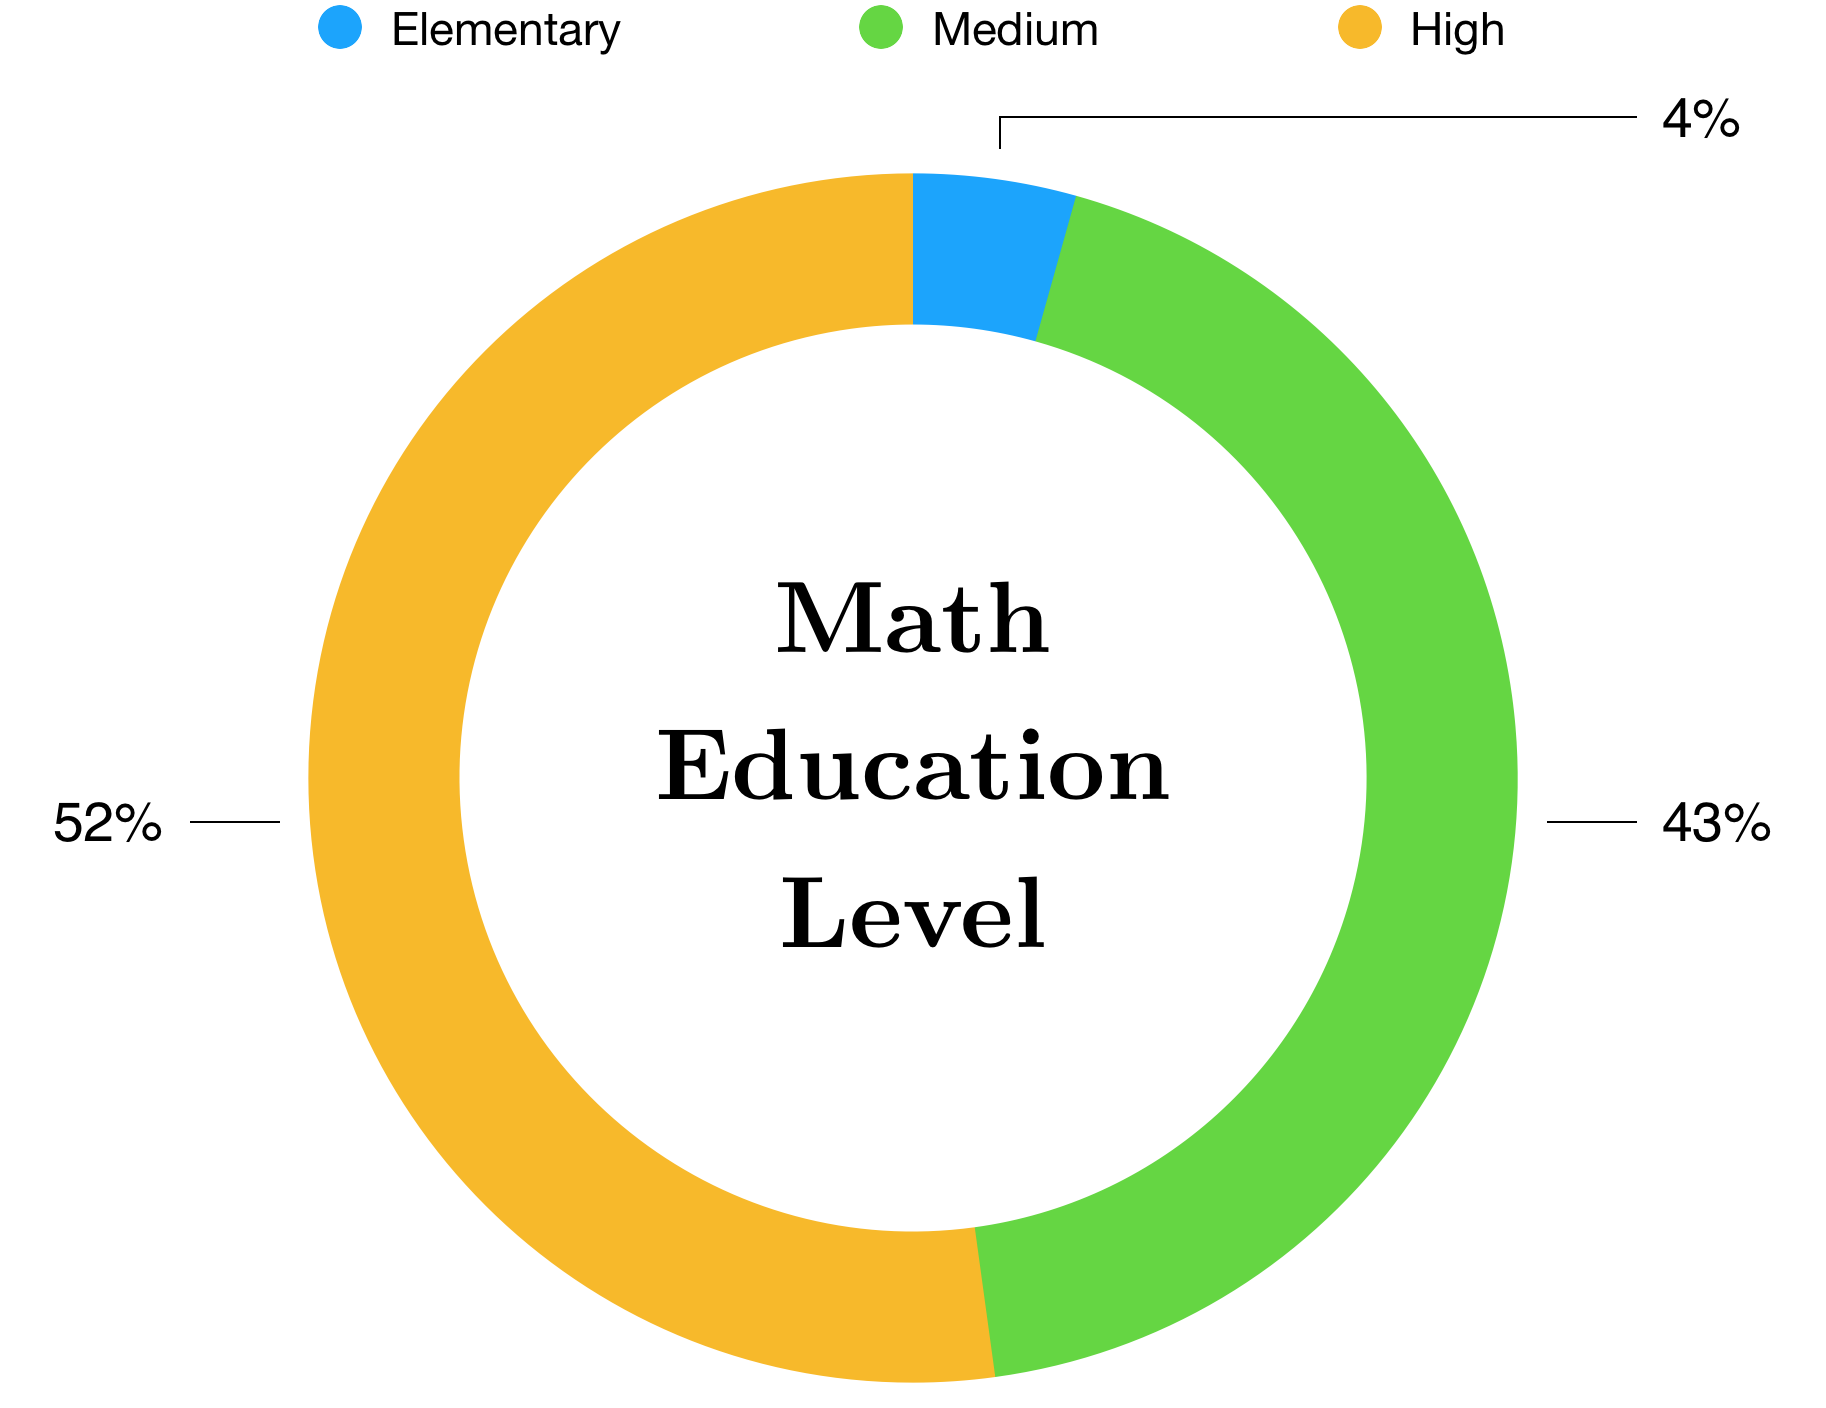
\includegraphics[width=0.4\textwidth]{MathEdLevel}
		}\\
		\subfigure[]{%
			\label{fig:Age}
			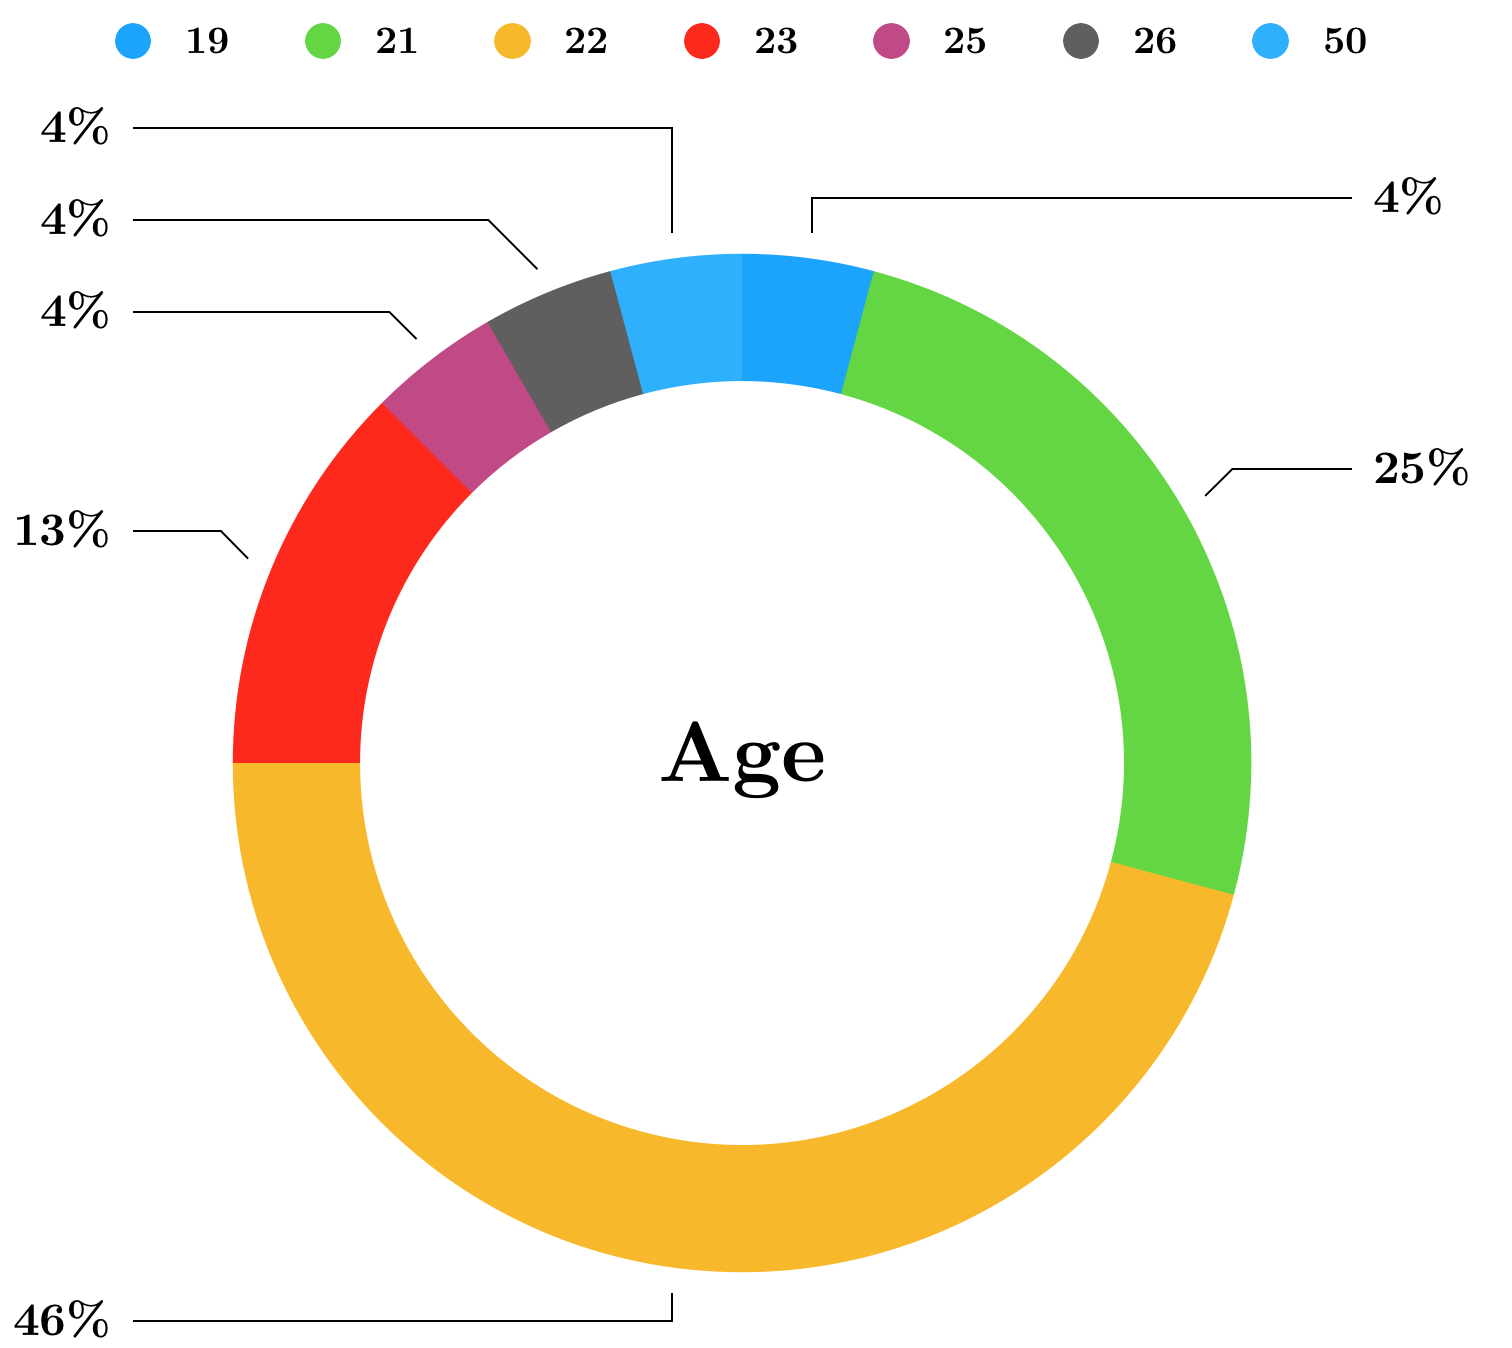
\includegraphics[width=0.5\textwidth]{Age}
		}		
	\end{center}
	\caption{
		Test Subjects' Attributes.
	}
	\label{fig:testSubjectsAttributes}
\end{figure}

In order to conduct the test, each one of the test subjects was placed in front of a personal computer. The following rules have been proposed :

\begin{itemize}
	\item \textit{You will be offered four different levels}.
	\item \textit{The first three levels will need to be repeated three times}.
	\item \textit{The last level can be executed only once}.
	\item \textit{Each level is a different $3d$-function}.
	\item \textit{Look carefully at the legend before starting the experiment}.
	\item \textit{At each click you will receive a score with a colour associated with it}.
	\item \textit{The goal is to make as many points as possible with $15$ clicks available for each game}.
	\item \textit{No further explanation will be provided}.
\end{itemize}

After that a chromatic scale (the legend) indicating how positive the reward was for each click, was proposed.

\begin{figure}[h!]
	\centering
	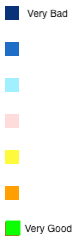
\includegraphics[height= 3 cm]{scala.png}
	\caption{Chromatic Scale.}
	\label{fig:Cromatic Scale}
\end{figure}

A white screen (with a specific hidden function) of $600 \times 600$ pixels with which to interact according to the rules previously listed was finally provided.

\begin{figure} [h!]
	\centering
	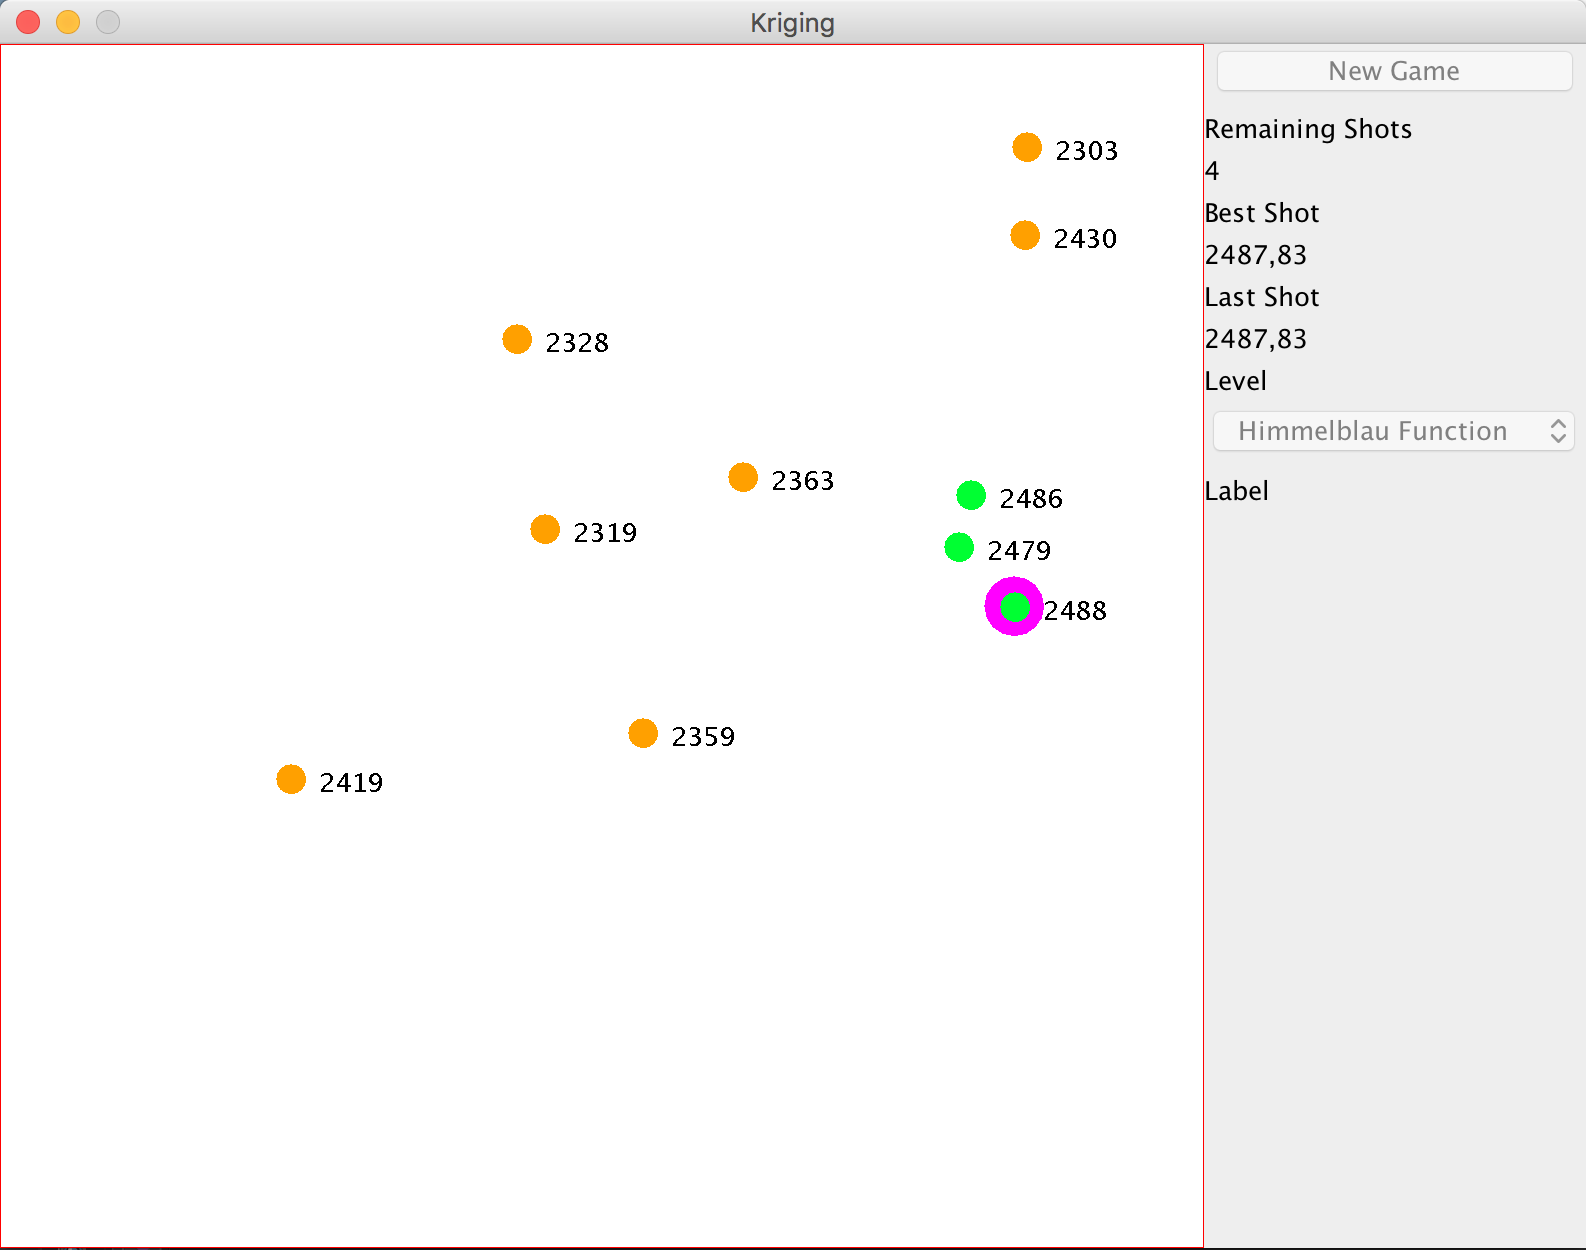
\includegraphics[width= \textwidth, height= 8 cm]{IMAGES/Form}
	\caption{GUI the player has to interact with during the experiment.}
	\label{fig:form}
\end{figure}







	\chapter{Results}

This chapter is divided into three sections. In the first section performances of the SARSA($\lambda$) algorithm, with the configuration are analysed. For each function results obtained applying the four different declinations of {\tt SARSA($\lambda$)} algorithm are compared. Remember that the four possible declinations are :

\begin{itemize}
	\item Linear, not random search
	\item Linear, random search
	\item Parametric, not random search
	\item Parametric, random search
\end{itemize}

Evaluations are made only on the greedy episode. The reason for this choice is to consider the algorithm's performances after giving a good enough training space composed by $150$ episodes, each one of $101$ epochs. \\

Three different plots for three different metrics are employed. The first one measures the \textit{Euclidean distance} \footnote{In mathematics, the Euclidean distance is the "ordinary" straight-line distance between two points in an Euclidean space. It is computed as follow: 
	
	\begin{equation}
		Euclidean\_distance = \sqrt{(x\textsubscript{i+n} - x_i)^2 + (y\textsubscript{i+n} - y_i)^2}
	\end{equation}

with $n \ge 0$. \\
	
Note that this performance metric is evaluated on the true function values but this information is not available for the optimization methods.} between point $(x_i, y_i)$ at epoch $e_i$, $\forall i \in n$ where $n$ is the number of epochs of greedy episode, and point $(x^*, y^*)$ which is the maximum. The second metric measures the \textit{function proximity in percentage} \footnote{The \textit{proximity in percentage} between the current value function and the optimal one is computed as follow:

\begin{equation}
Proximity\_in\_ percentage = \frac{currentValueFunction \times 100}{optimalValueFunction}
\end{equation}

Note that this performance metric is evaluated on the true function values but this information is not available to the optimization methods. \\ } between the current value function and the optimal one in the greedy episode. The third one represents the \textit{Gap metric}\footnote{This metric measures how effective each method is at finding the global maximum.

\begin{equation}
G_t = \dfrac{f(x^+, y^+) - f(x_1, y_1)}{f(x^* y^*) - f(x_1, y_1)}
\end{equation}

Where $x^+$ is the incumbent or best function sample found up to epoch $e$. The gap $G_t$ will therefore be a number between $0$ (indicating no improvement over the initial sample) and $1$ (if the incumbent is the maximum). Note that this performance metric is evaluated on the true function values but this information is not available to the optimization methods.~\cite{Hoffman:2011:PAB:3020548.3020587}} computed on the greedy episode. \\

In the second section a second experiment conducted adopting an \textit{experienced} version of the SARSA($\lambda$) algorithm will be described. In this case the algorithm is trained on different functions and evaluations are made on the greedy episode of the Styblinski-Tang's Revised function, run only using \textit{experience} acquired on other functions with no specific training on the function itself. \\

In the third section results obtained from experiment conducted on humans will be analysed.

\section{Basic SARSA($\lambda$) Algorithm's Performances}

\begin{figure}[h!]
	\begin{center}
		\subfigure[]{%
			\label{fig:HimmelblauDifference}
			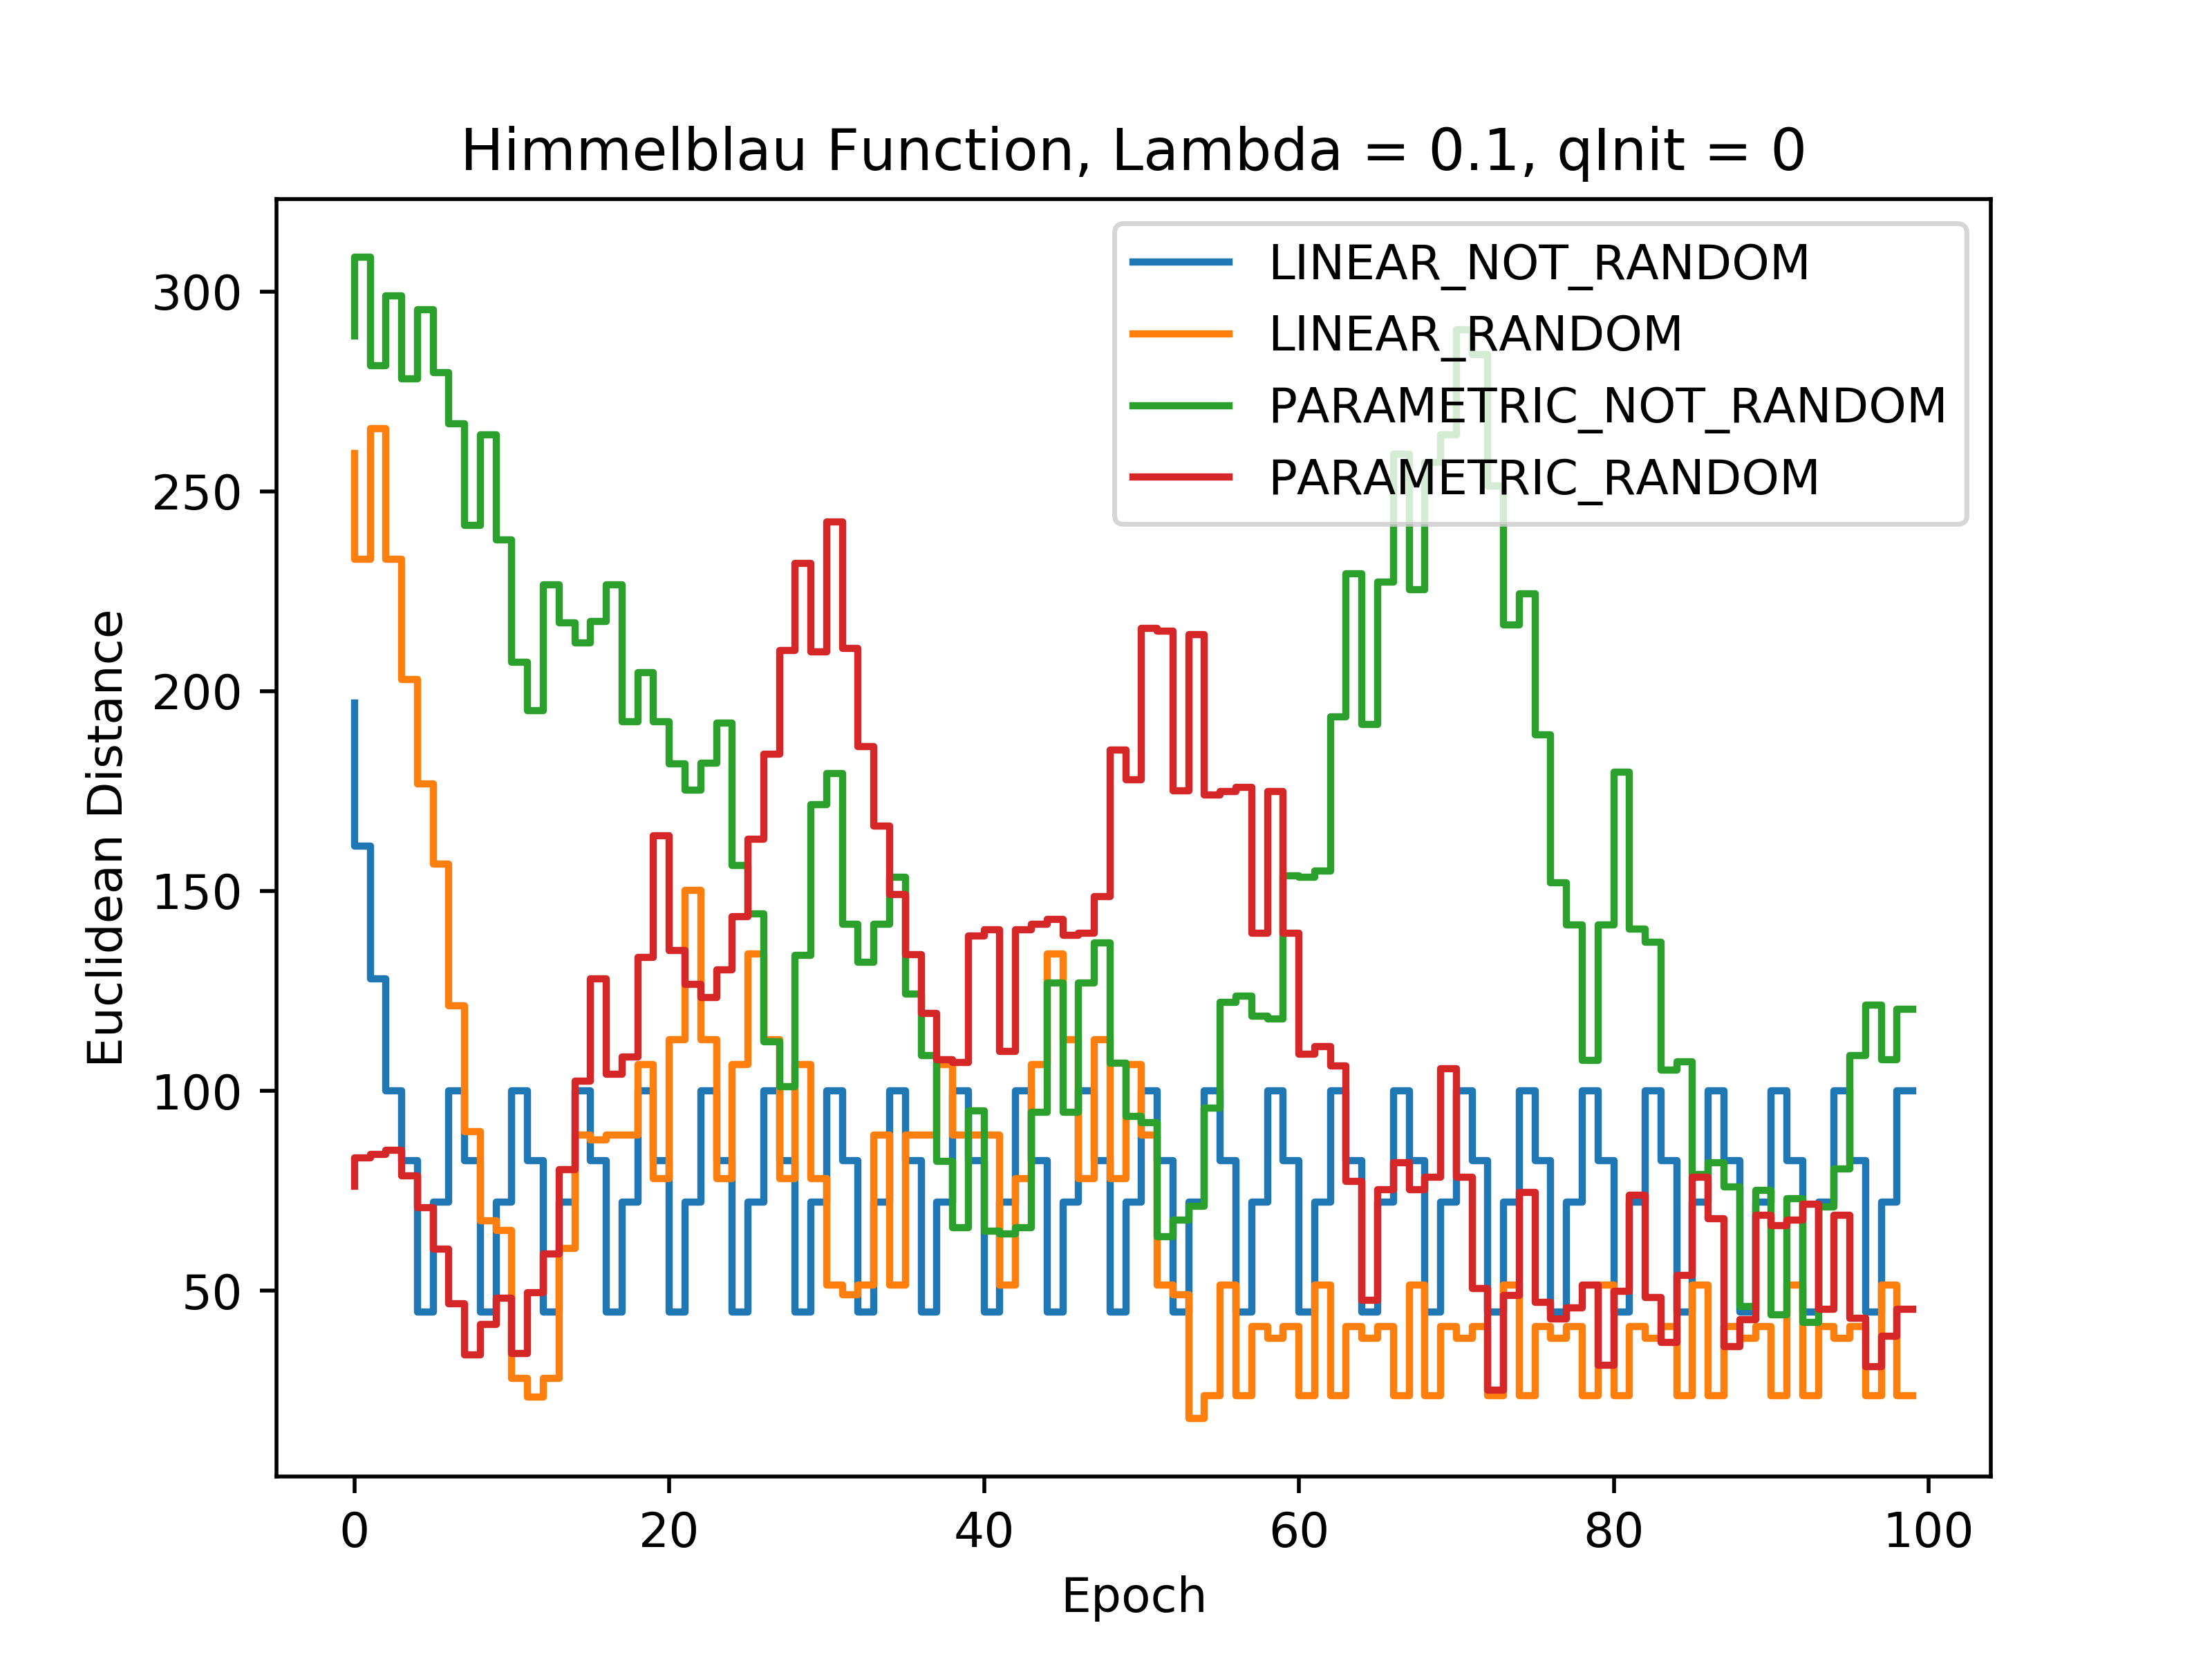
\includegraphics[width=0.4\textwidth]{HimmelblauDifference}
		}
		\subfigure[]{%
			\label{fig:HimmelblauValueFunction}
			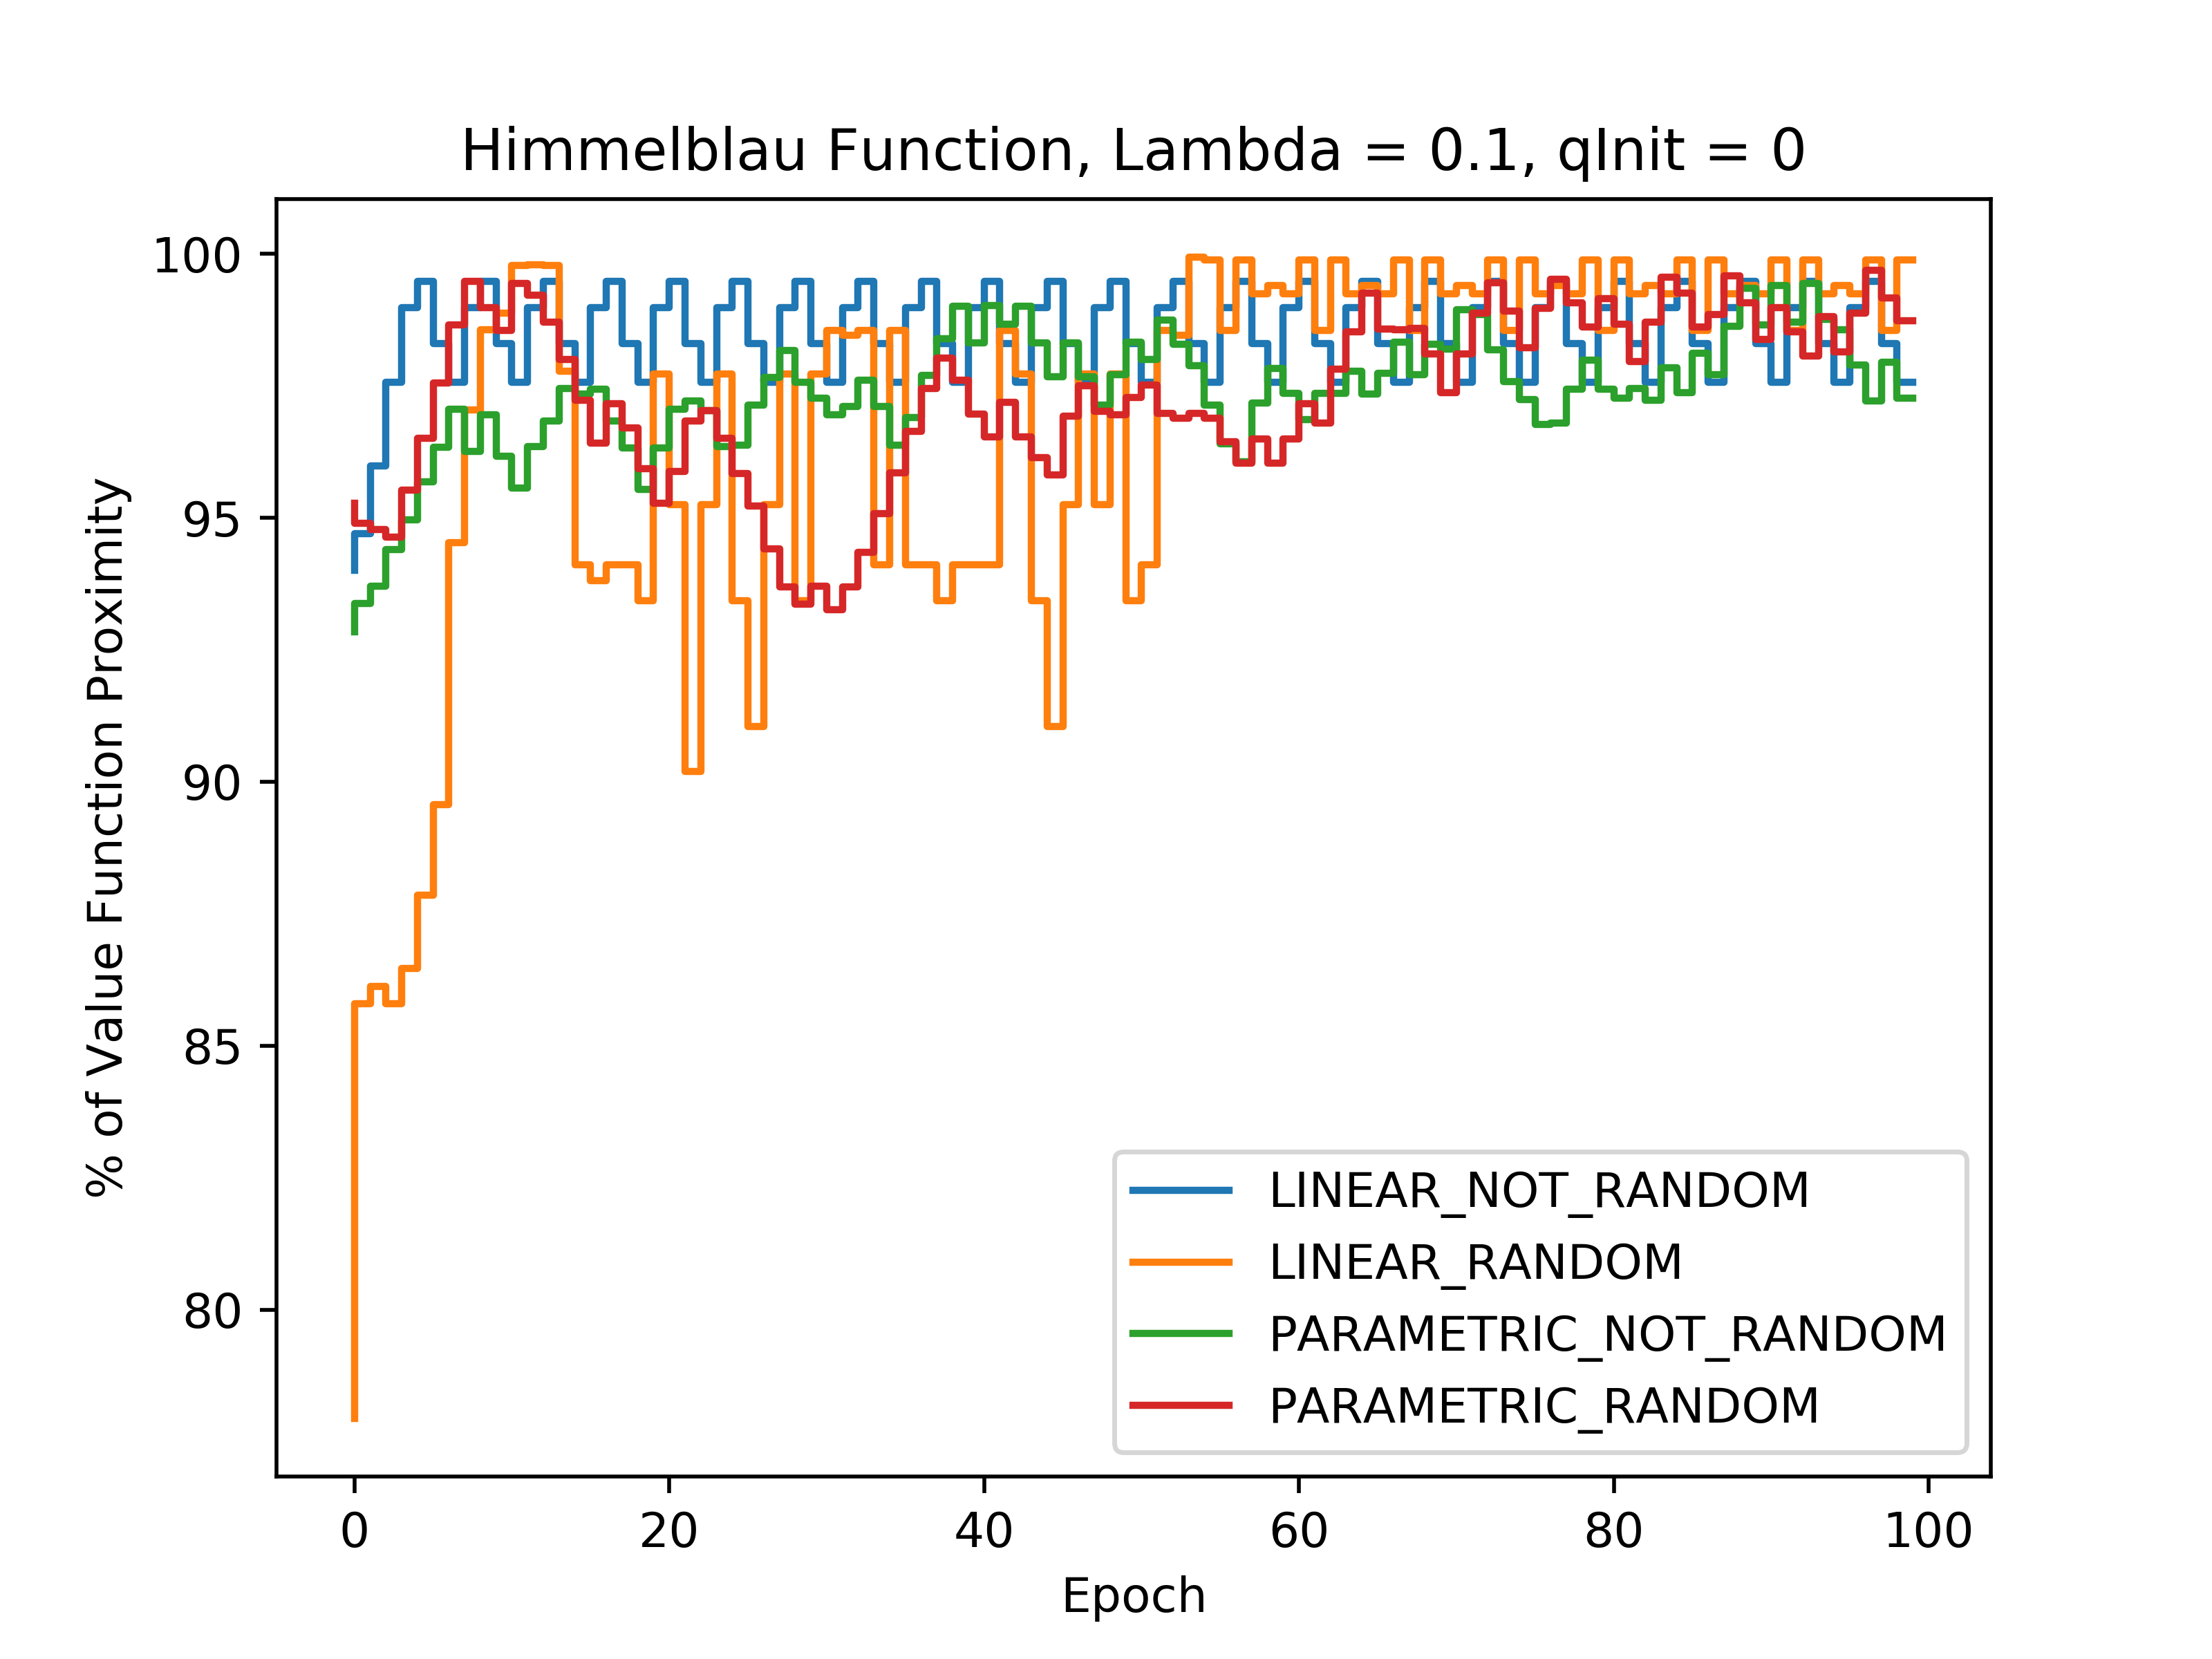
\includegraphics[width=0.4\textwidth]{HimmelblauValueFunction}
		}\\
		\subfigure[]{%
			\label{fig:HimmelblauGap}
			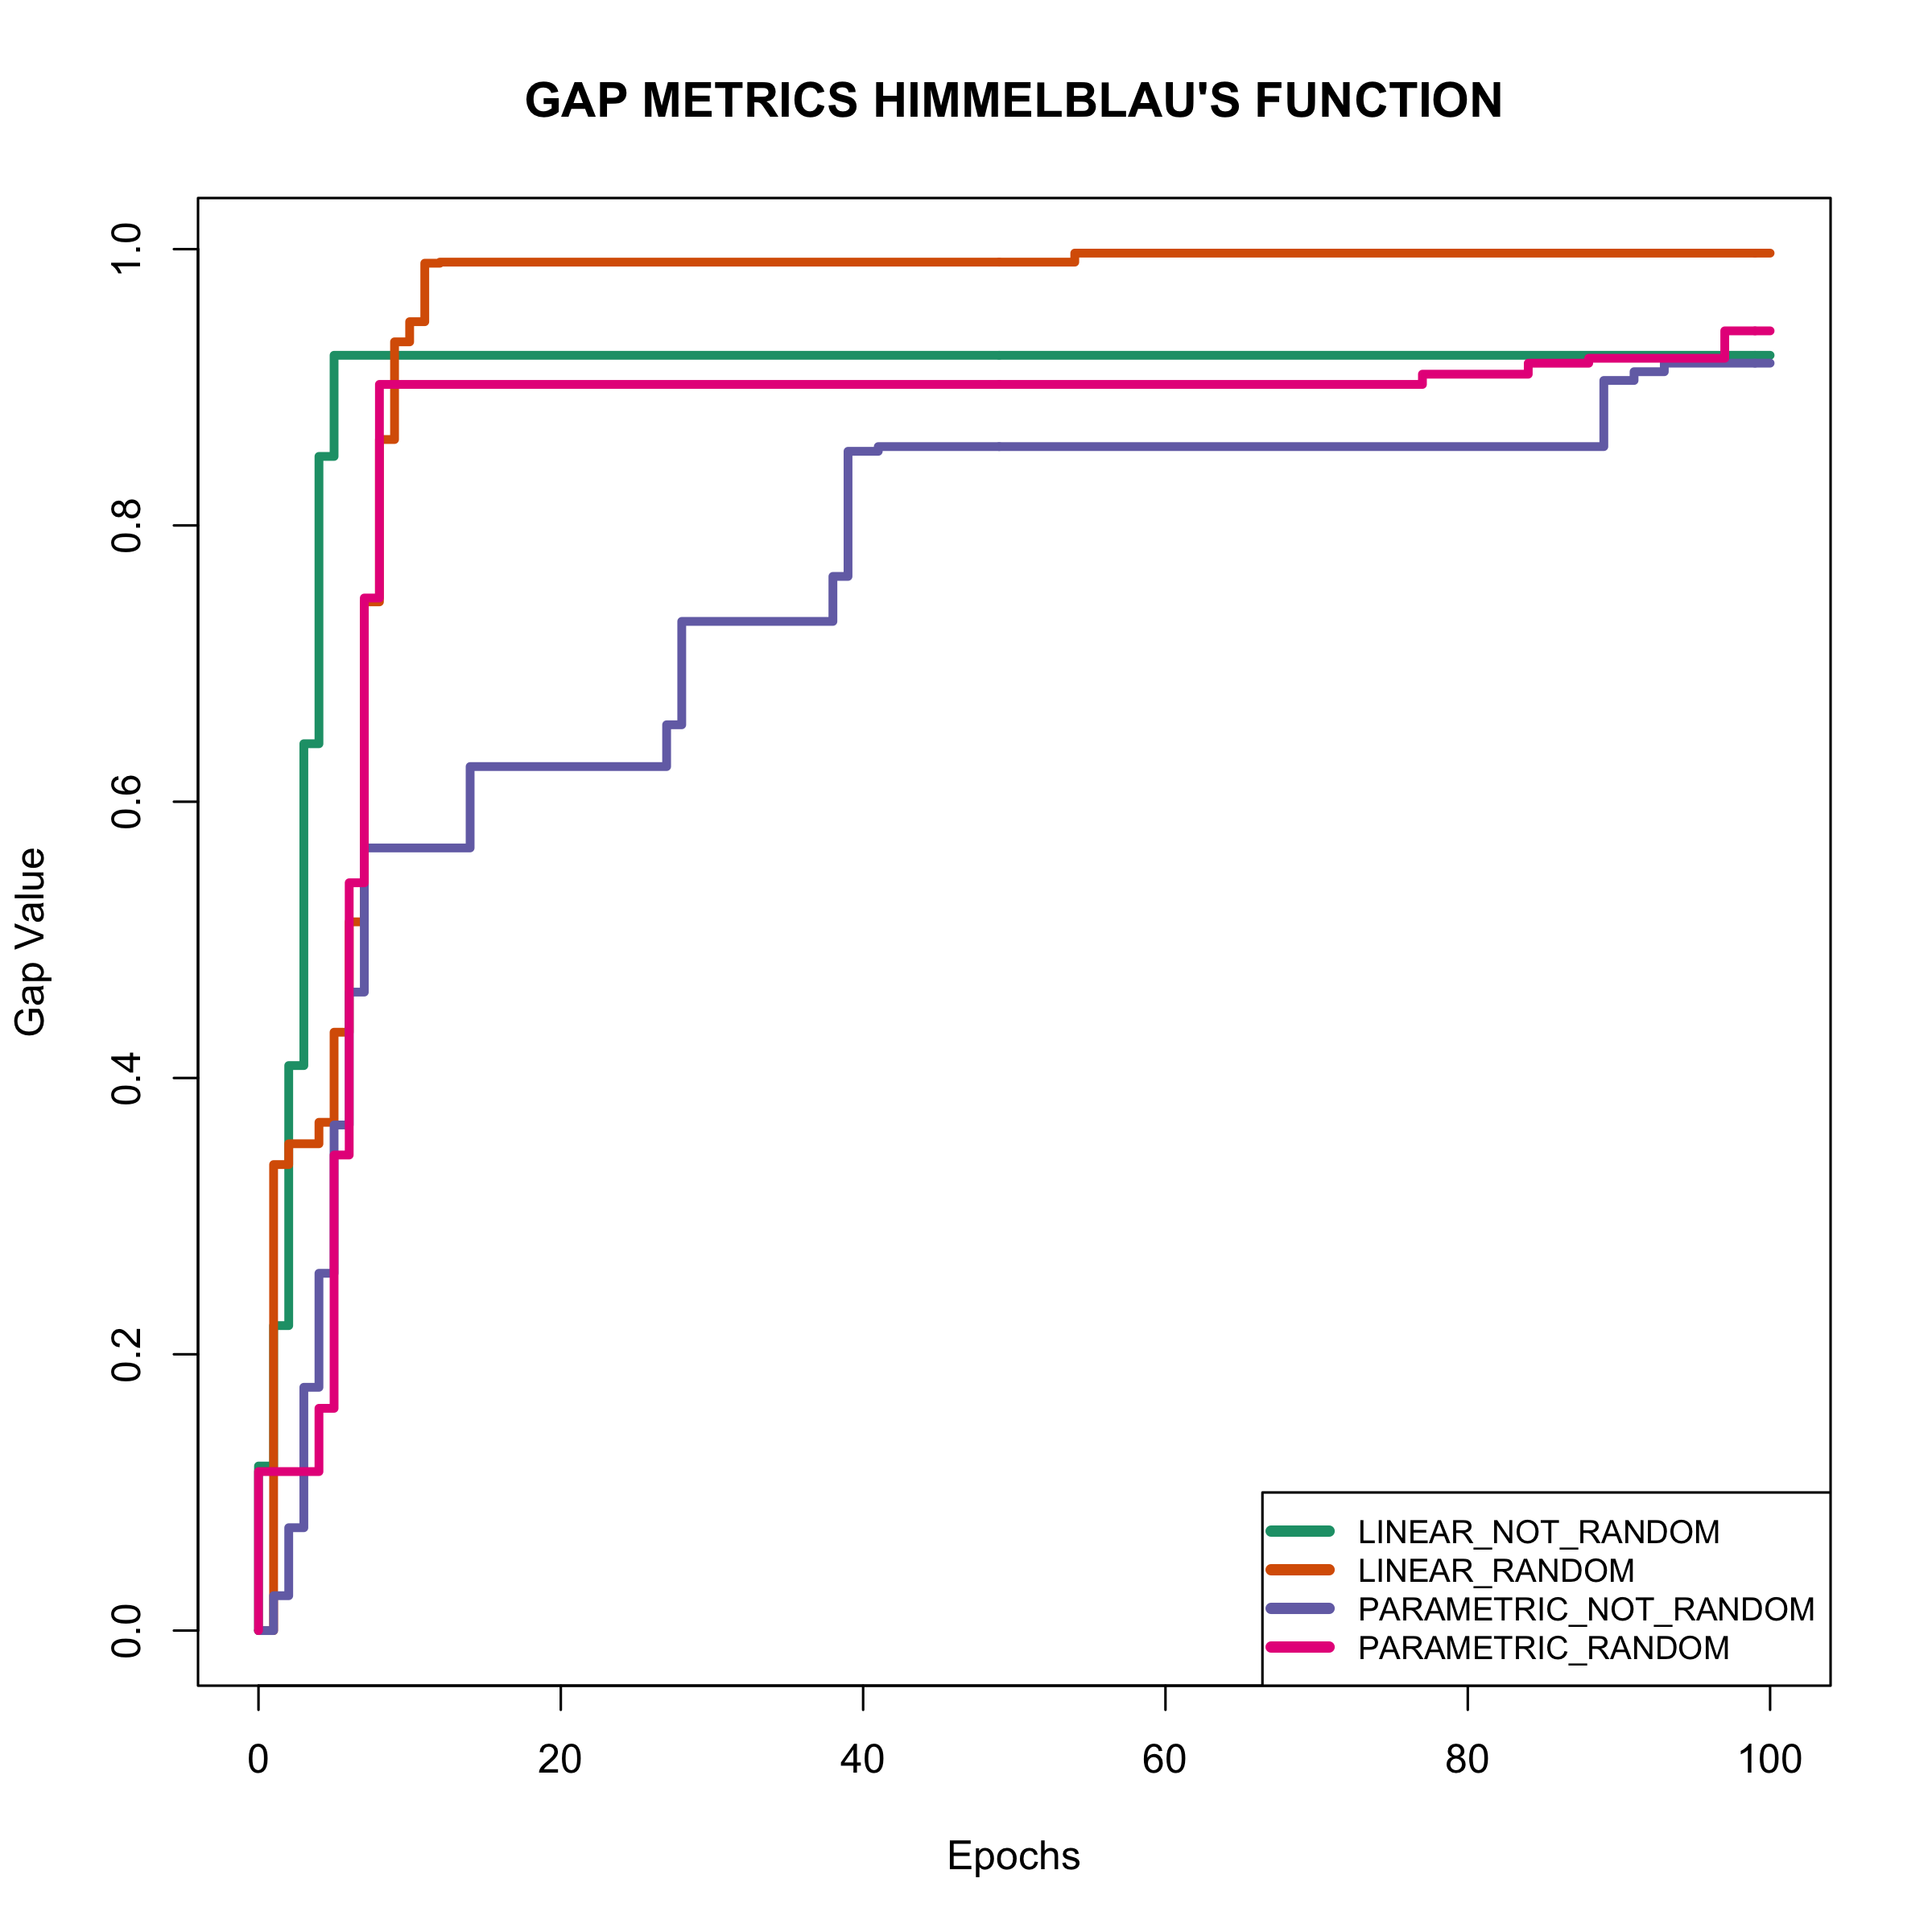
\includegraphics[width=0.4\textwidth]{HimmelblauGap}
		}		
	\end{center}
	\caption{
		Himmelblau' s Function.
	}
	\label{fig:HimmelblauResults}
\end{figure}

\subsection{Himmelblau' s Function} Plot (a) of figure \ref{fig:HimmelblauResults} graphically represents performances of the four possible declinations of {\tt SARSA($\lambda$)} algorithm obtained considering the \textit{Euclidean distance metric}. 

Looking at the {\tt linear, not random} declination's performance, it can be possible to note a starting high Euclidean difference between the agent's position and the global maximum. It decreases until epoch $5$. Starting from this epoch, a recurrent pattern starts to be developed. This behaviour depends on the fact that once the agent has achieved a good position compared to the maximum, it has to continue to make movements until the terminal state is achieved. Each movement implies a reward. The agent selects a set of movements that maximizes the reward and systematically repeats them. The stability just described is also proved by the fact that the standard deviation of the current declination is the lowest of the set with a value of $25.3$ (table $5.1$).

{\tt Linear, random} declination has a greater instability compared to the {\tt linear, not random} one. In the first fifty epochs the \textit{Euclidean distance} from the global maximum is constantly higher but then it starts to stabilize. Starting from the fiftieth epoch it develops a recurrent pattern and achieves best results. With an Euclidean distance mean of $71.6$ pixels from the maximum, it has the best performance of the set (table $5.1$).

The {\tt parametric, not random} declination has worst performances of the declinations' set. It is unable to minimize the Euclidean distance from the global maximum and it is highly unstable. Looking at table $5.1$ it is possible to note that the current declination as highest values in all statistic measures.

Finally, the {\tt parametric, random} declination selects a starting point near to the global maximum but it is unable to maintain a low Euclidean distance from it until epoch seventy. Starting from this epoch it develops a recurrent pattern similar to one previously described. Despite of this it is possible to say that its performances are worse compared to the first two ones.

Slower convergence of linear declinations compared to parametric ones depends on the fact that in the first case, as already explained in \textbf{Chapter $3$}, greater movements are done at each epoch and a lower training time is required to achieve the maximum. The amount of parametric movements are strictly conditioned by the function's shape. If this represents an obstacle to a fast convergence, however it is an incentive to an higher precision. \\

\begin{table} [h!]
	\centering
	\resizebox{\linewidth}{!} {
	\begin{tabular}{c| cccccc}
		\hline \textbf{Himmelblau' s Function}
		& \textbf{Mean (pixels)} & \textbf{Standard deviation}  \\ 
		\hline Linear not Random
		& $77.7$ &\cellcolor{red!25}$25.3$ \\ 
		\hline Linear Random
		& \cellcolor{red!25}$71.6$ & $52.2$ \\ 
		\hline Parametric not Random
		& $158.6$ & $71.3$ \\ 
		\hline Parametric Random
		& $105.5$ & $56.0$ \\ 
		\hline 
	\end{tabular}
}
\label{tab:HimmelblauTabEuclidean}
\caption{Euclidean Metric's Performances}
\end{table}

Plot (b) of figure ~\ref{fig:HimmelblauResults} graphically represents performances of the four possible declinations of {\tt SARSA($\lambda$)} algorithm obtained considering the \textit{Function Proximity in Percentage} metric.

All declinations, except for the {\tt linear, random} one, start with an high level of value function's proximity to the maximum. It depends on the function's shape. 

Once it has achieved a good enough proximal point to the maximum, the {\tt linear, not random} declination maintains always the same vale function's proximity level developing a recurrent pattern. The average level of proximity achieved by this declination is the best of the set (table $5.2$). The high stability of the current declination is proved by the lowest standard deviation of the set (table $5.2$). 

The {\tt linear, random} declination starts from a point not very close to the maximum in terms of value function's value. Its great instability reveals an inadequate training space. It starts to stabilize starting from the fiftieth epoch. Its starting instability is proved by the highest standard deviation of the set (table $5.2$).

The {\tt parametric, not random} declination reveals a general stability. The growth of proximity is slower then the corresponding linear declination because of the reduced amount of movement depending on the function's shape. 

Finally, the {\tt parametric, random} declination, as the corresponding linear declination, shows an initial instability. In general performances are more stable than the linear corresponding ones because of the lower amount of movement done at each epoch. Starting from the sixty-fifth epoch the proximity slowly grows and stabilizes. \\

\begin{table} [h!]
	\centering
	\resizebox{\linewidth}{!} {
	\begin{tabular}{c| cccccc} 
		\hline \textbf{Himmelblau' s Function}
		& \textbf{Mean (\%)} & \textbf{Standard deviation}  \\ 
		\hline Linear not Random
		& \cellcolor{green!25}$98.5$ & \cellcolor{green!25}$0.96$  \\ 
		\hline Linear Random
		& $96.8$ & $4.0$ \\ 
		\hline Parametric not Random
		& $97.4$ & $1.2$ \\ 
		\hline Parametric Random
		& $97.3$ & $1.6$ \\ 
		\hline 
	\end{tabular}
}
\label{HimmelblauTabProximity}
\caption{Function Proximity in Percentage.} 
\end{table}

Plot (c) of figure ~\ref{fig:HimmelblauResults} graphically represents performances of the four possible declinations of {\tt SARSA($\lambda$)} algorithm obtained considering the \textit{Gap metric}. According to this plot the most effective declination of {\tt SARSA($\lambda$)} algorithm in finding the maximum is the {\tt linear, random} one. Looking at table $5.9$ it is possible to note that {\tt linear, random} declination achieves point $(3.67, -1.57)$ with a value function of $2498.457$ out of $2500.0$.

\begin{figure}[h!]
	\begin{center}
		\subfigure[]{%
			\label{fig:ParabolicDifference}
			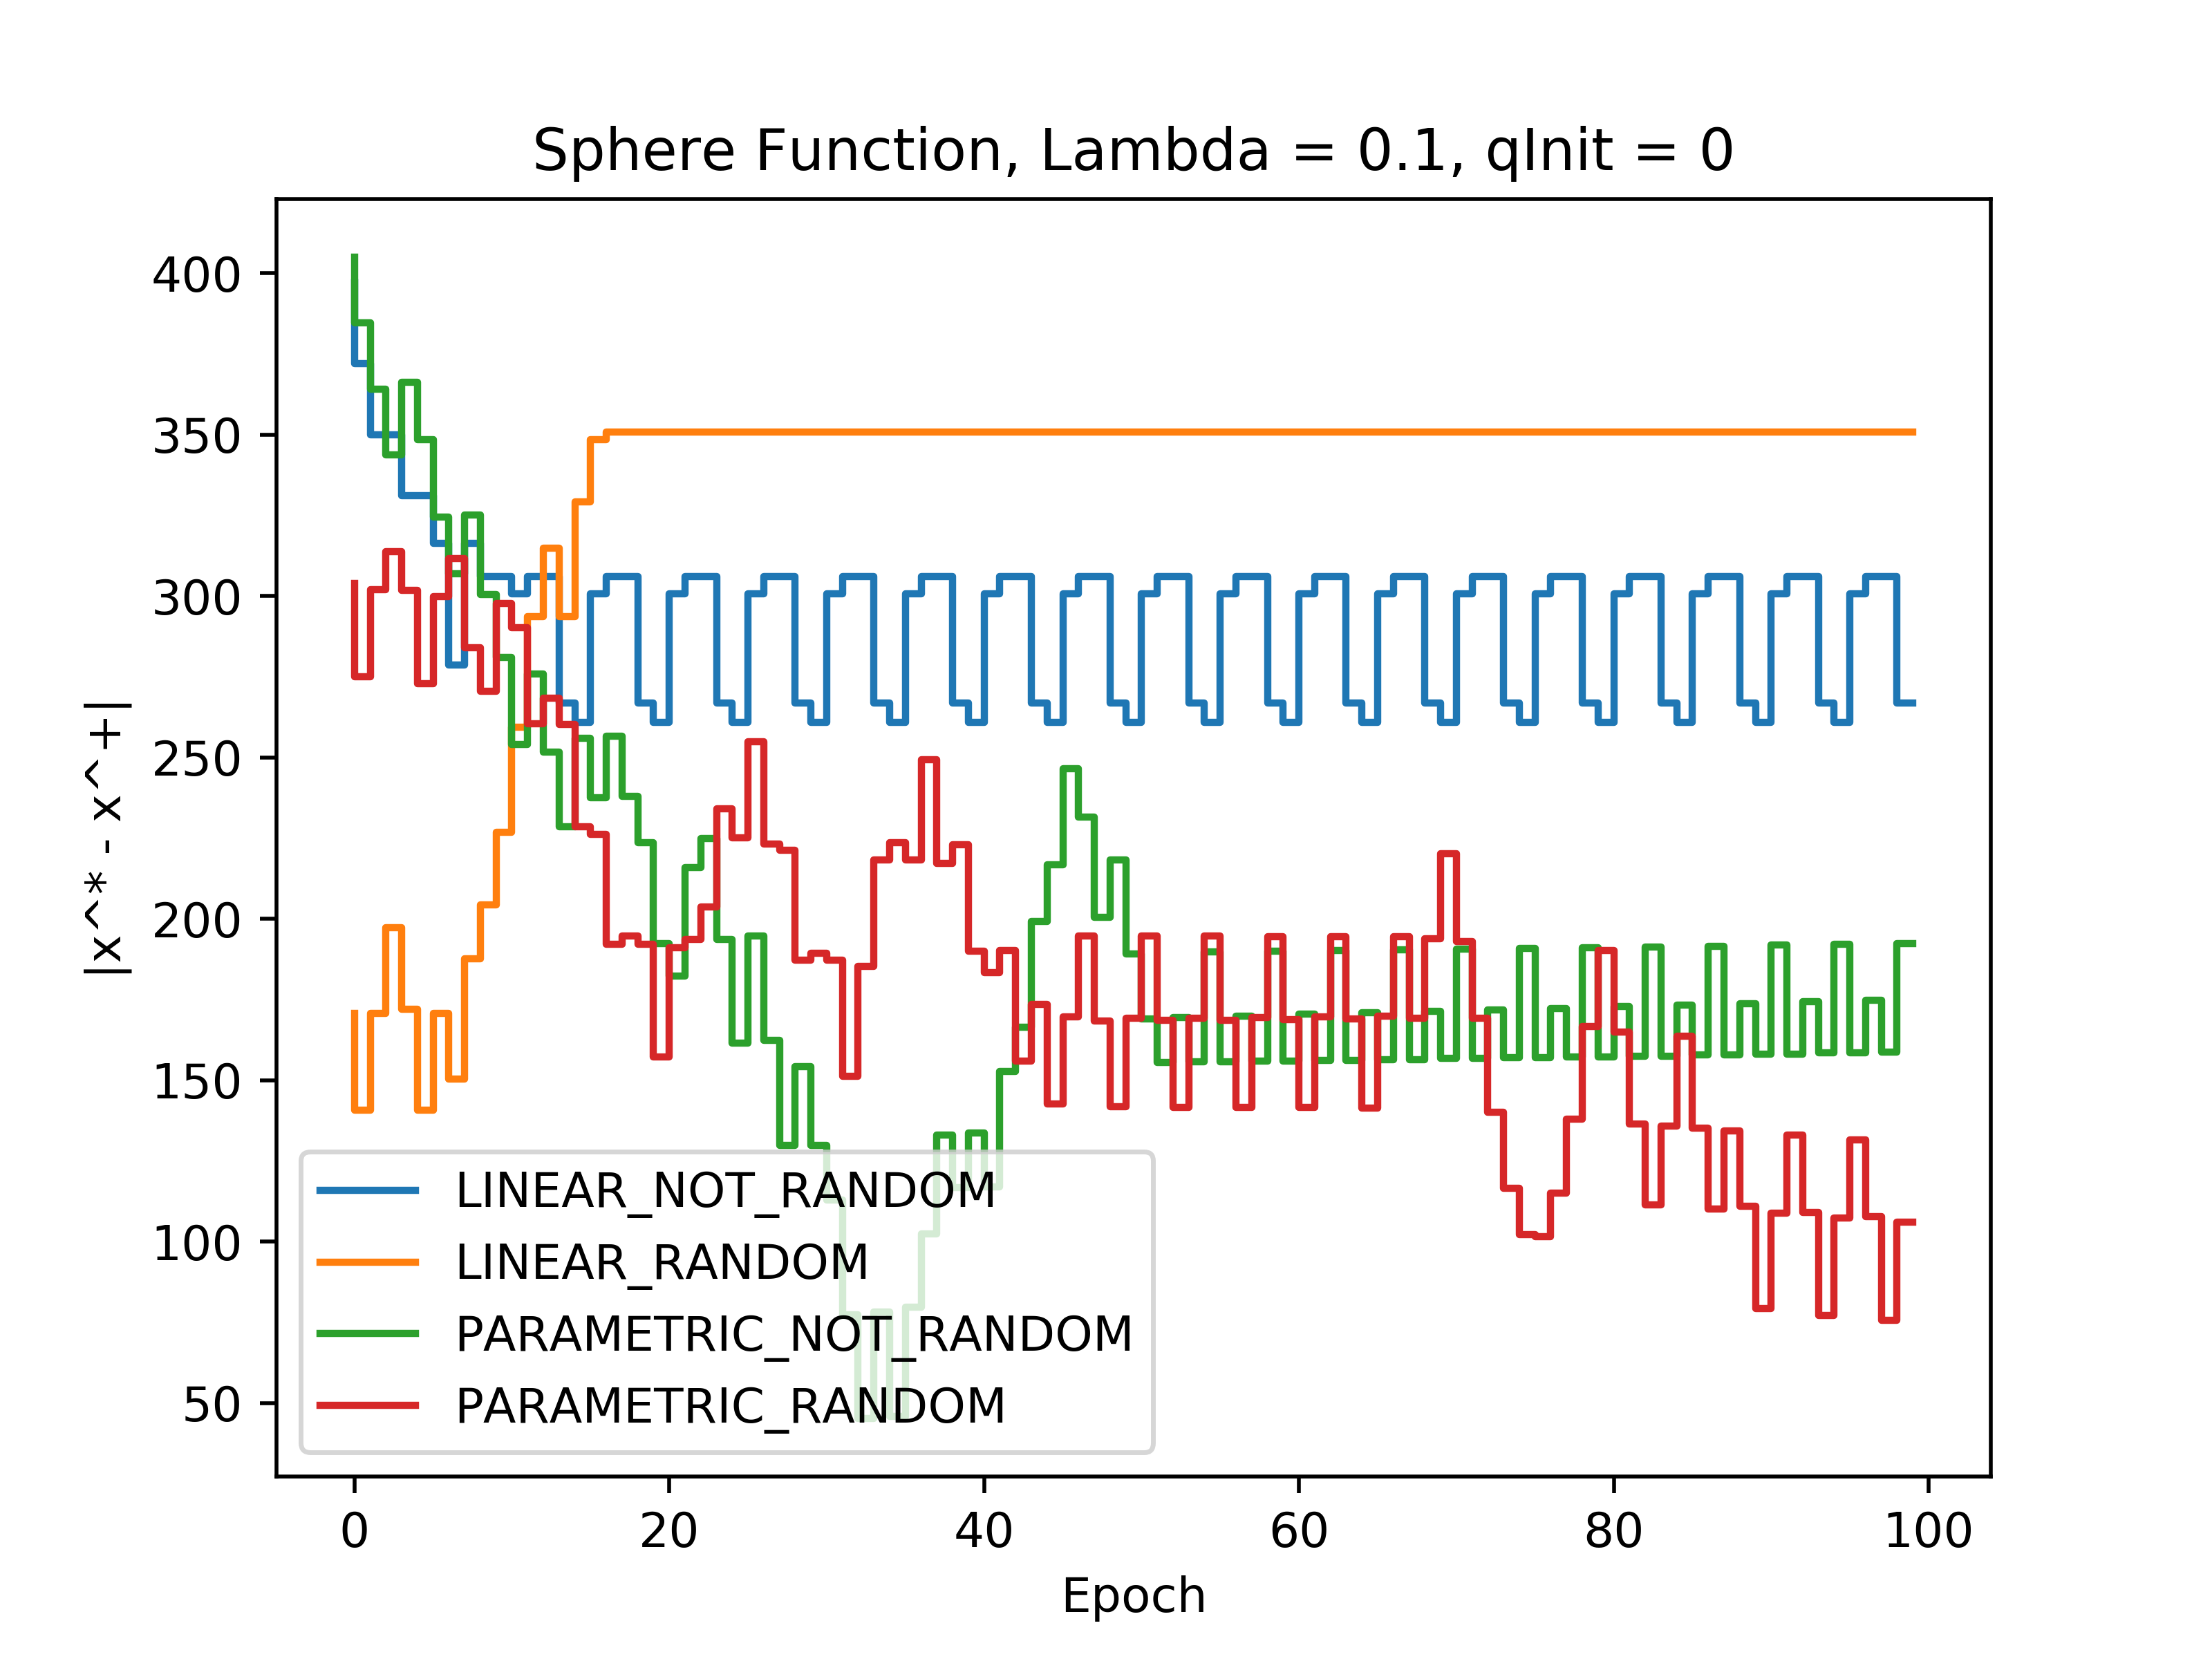
\includegraphics[width=0.4\textwidth]{ParabolicEuclidean}
		}
		\subfigure[]{%
			\label{fig:ParabolicValueFunction}
			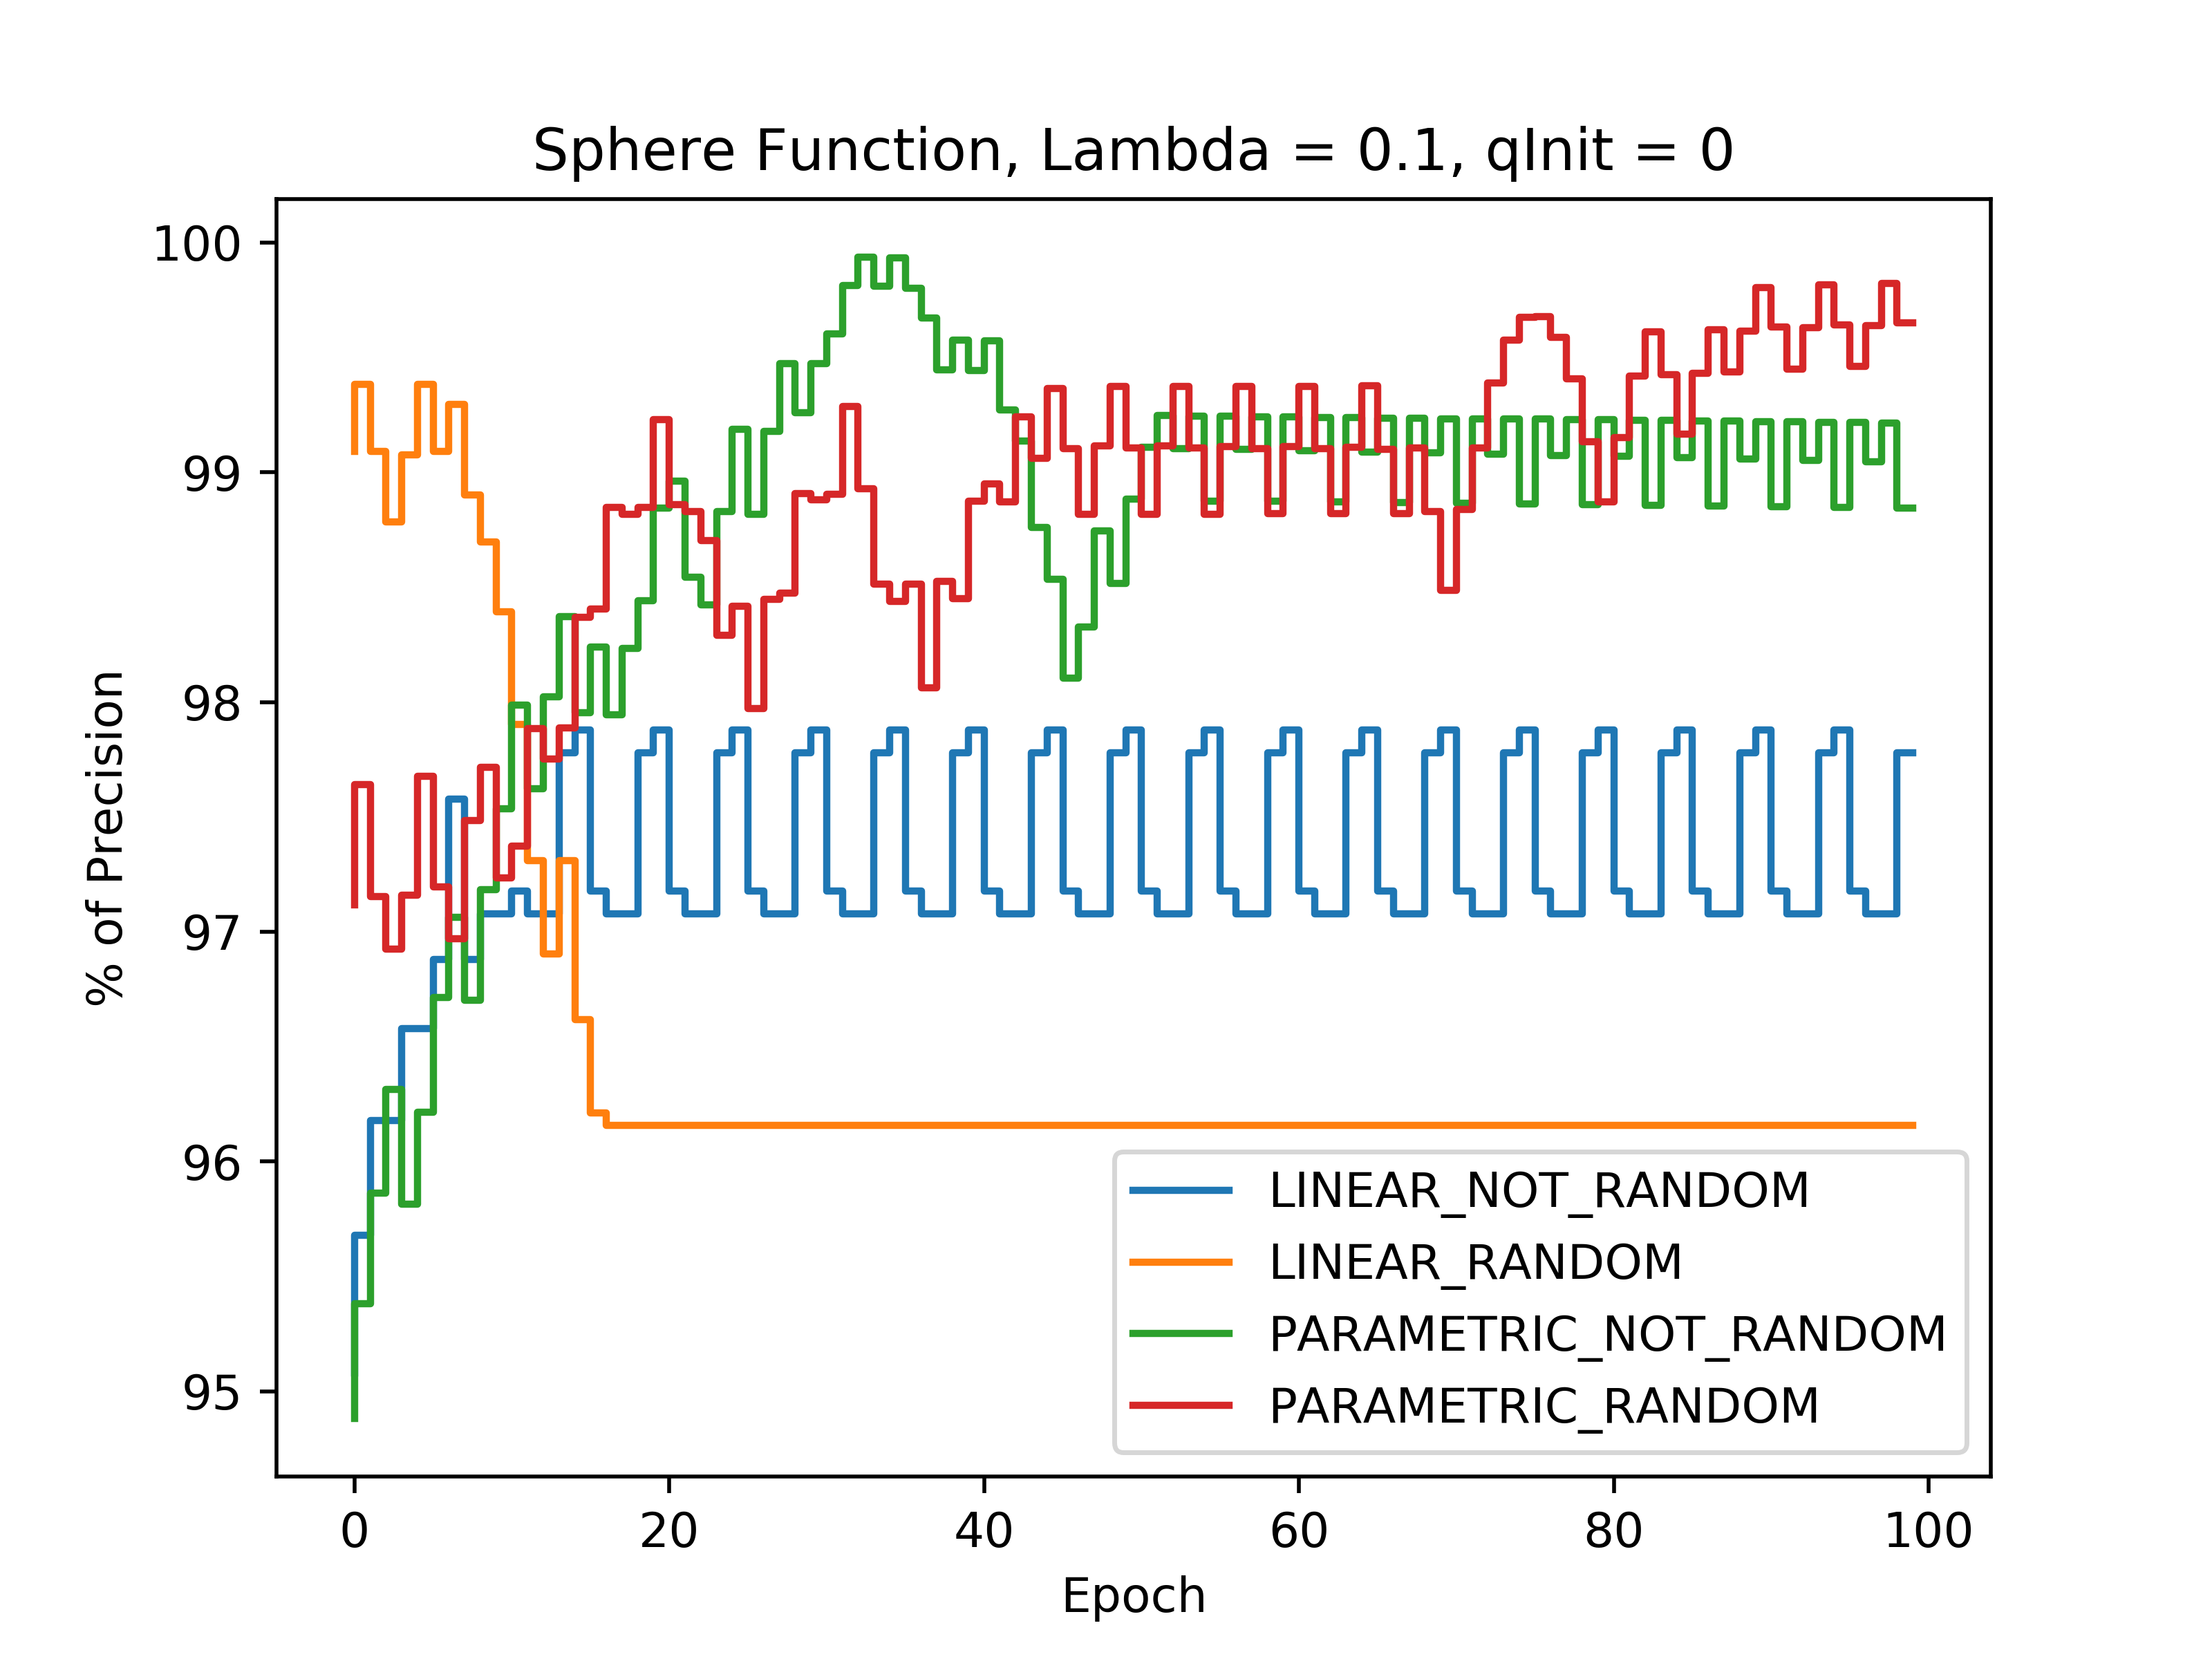
\includegraphics[width=0.4\textwidth]{SphereValueFunction}
		}\\
		\subfigure[]{%
			\label{fig:ParabolicGap}
			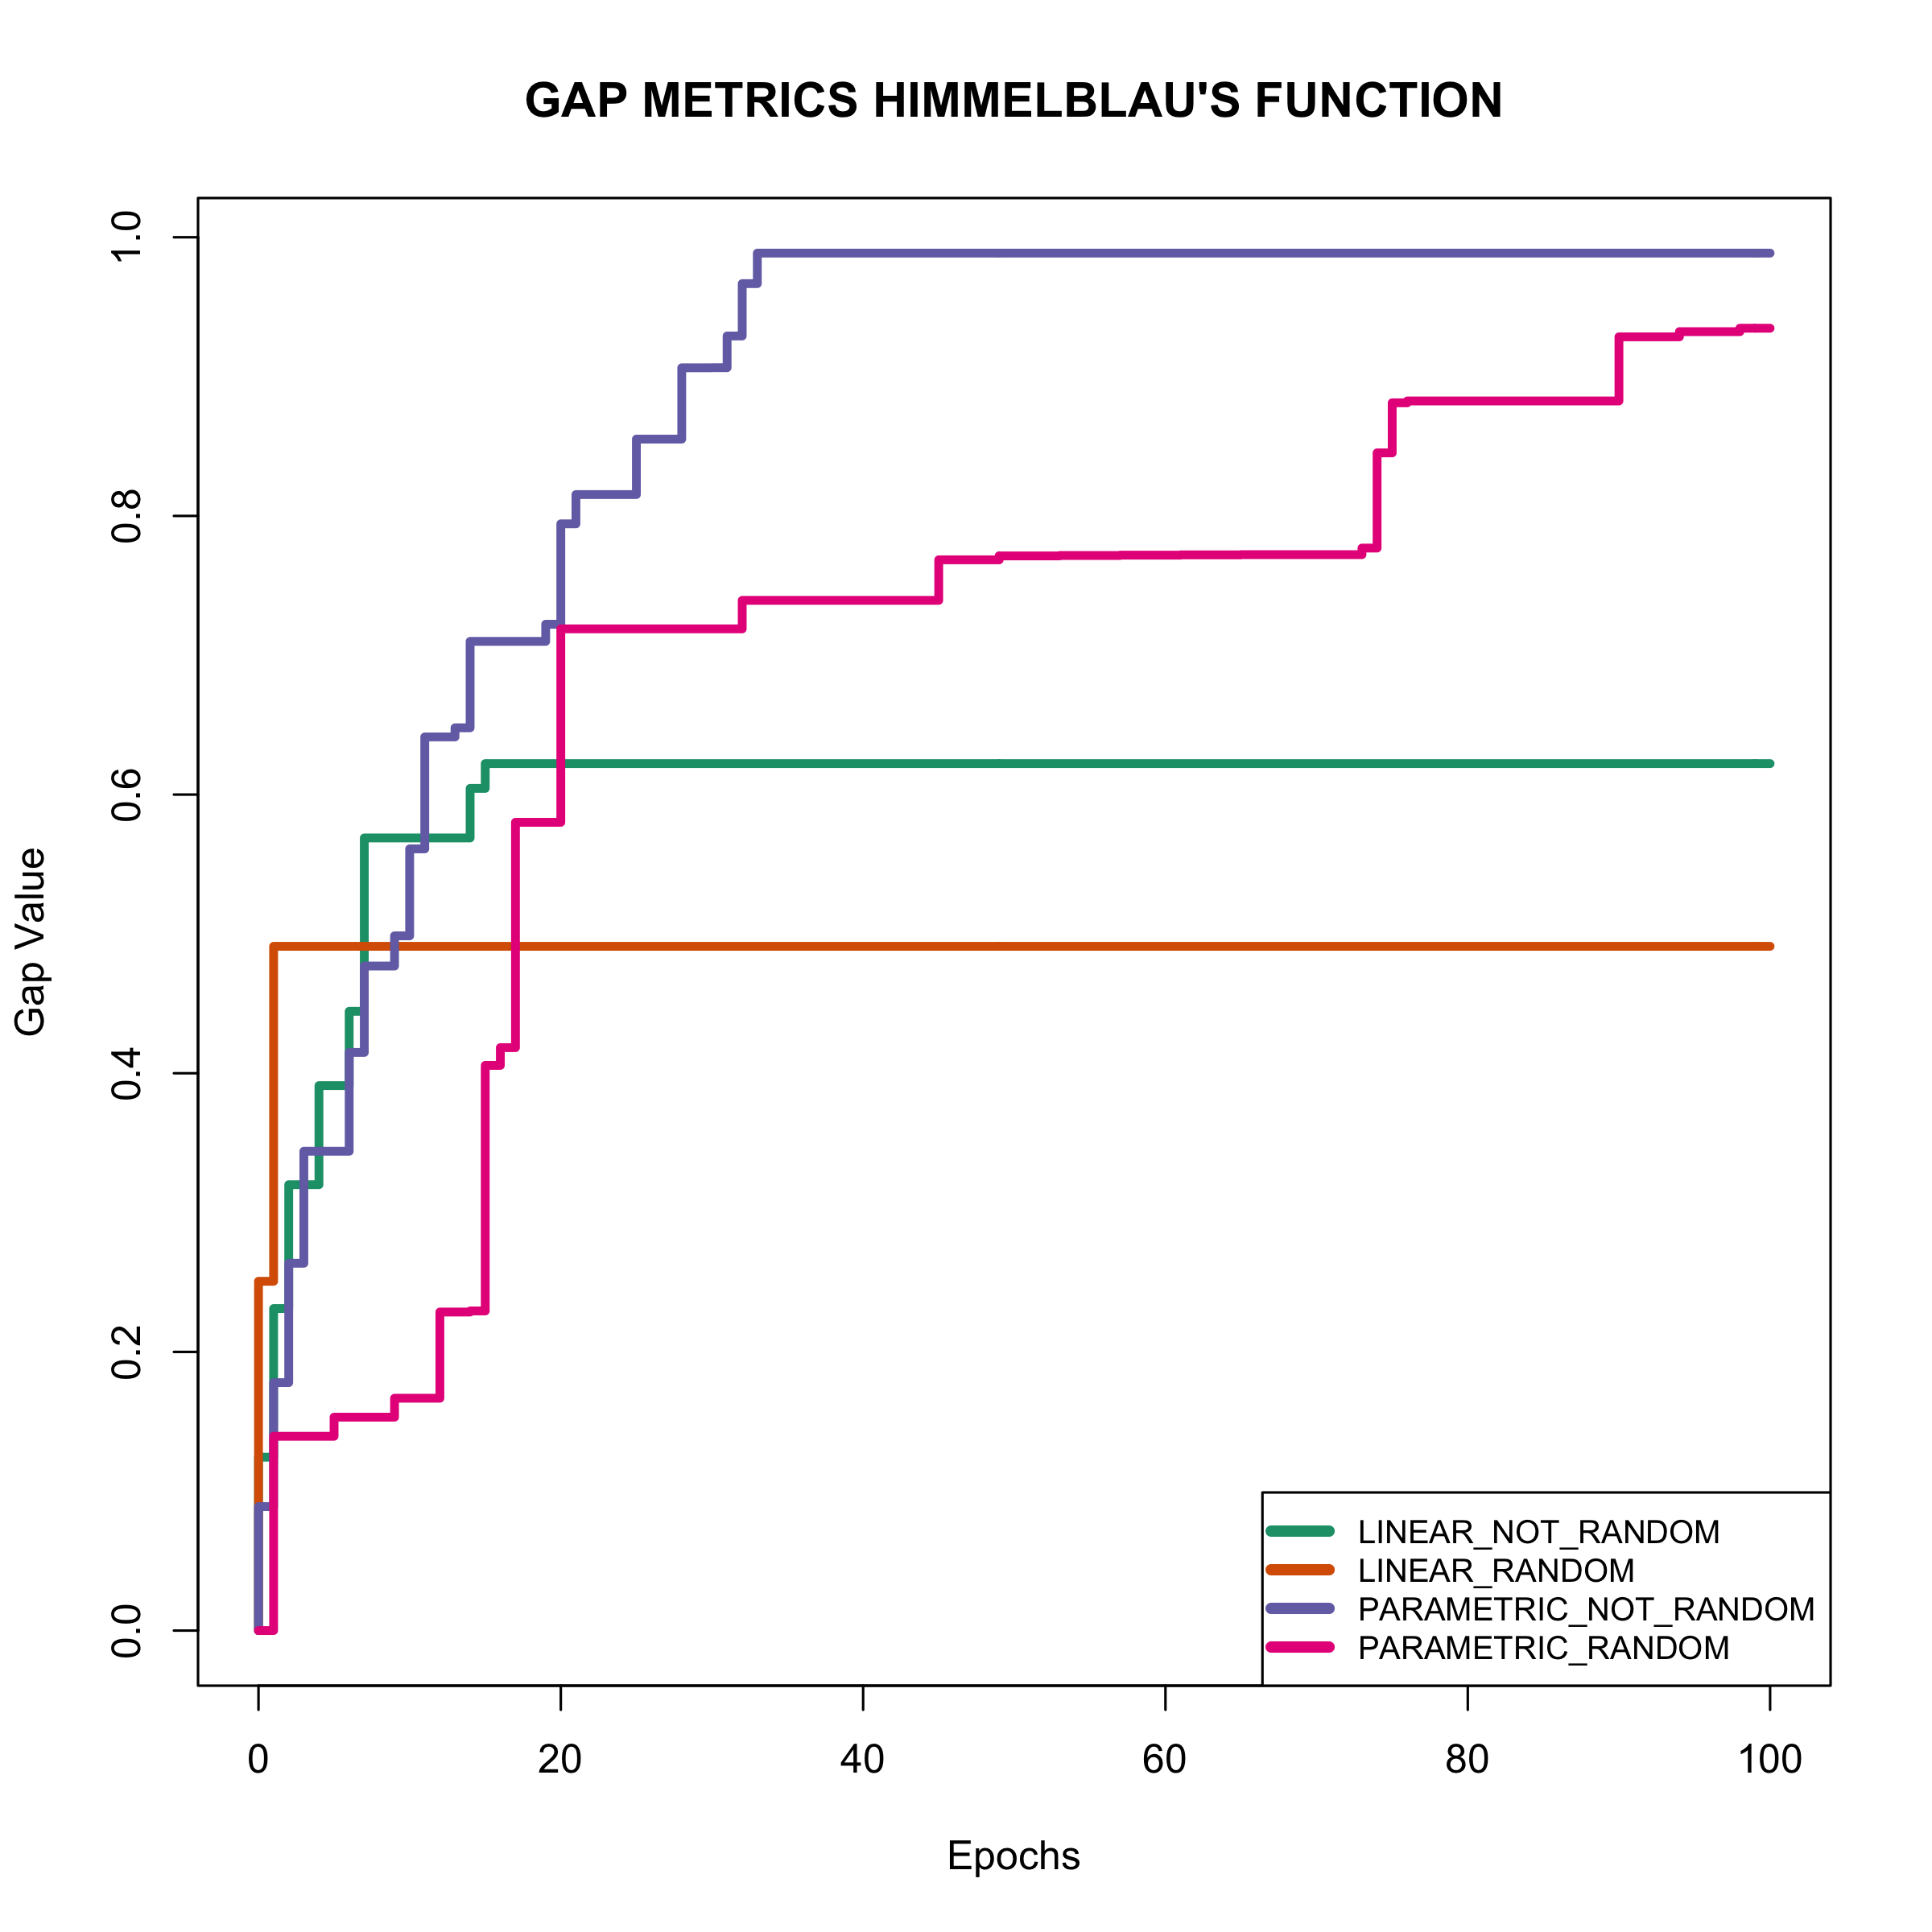
\includegraphics[width=0.4\textwidth]{ParabolicGap}
		} \\
		
	\end{center}
	\caption{
		Sphere Function.
	}
	\label{fig:ParabolicResults}
\end{figure}


\subsection{Sphere Function} Before starting to analyse performances of different declinations of {\tt SARSA($\lambda$)} algorithm in maximizing the Sphere function, it is important to underline that the starting point for the current function in non-random declinations is $(0, 0)$. The reason for this choice is that $f(300, 300)$ is itself the maximum of the function. \\

Plot (a) of figure ~\ref{fig:ParabolicResults} graphically represents performances of the four possible declinations of {\tt SARSA($\lambda$)} algorithm obtained considering the \textit{Euclidean distance metric}. Looking at the {\tt linear, not random} declination it is possible to note a constant, high Euclidean difference between the agent's position and the global maximum. This distance never decreases and still from the first epochs, a recurrent pattern starts to be developed. The inefficiency of the algorithm's declination depends on an inadequate training space. The relationship between different explored states and total possible states does not permit the agent to develop an efficient policy. Bad performance's results of the current declination are also certified by an high metric's average (table $5.3$). On the other hand the great stability of this declination is underlined by the lowest standard deviation of the set (table $5.3$).

{\tt Linear, random} declination starts from a point relatively close to the maximum, but, one more time, the inadequate training space prevents its to develop a rally optimal policy. This declination is the less efficient one with an average Euclidean distance from the maximum of $328.9$ pixels.

Better performances can be registered looking at parametric declinations of the algorithm. The {\tt parametric, not random} declination starts with a physiological high Euclidean difference from the maximum. It rapidly decreases until the thirty-fifth epoch and then it has another soft increase. Starting from the fifty-fifth epoch a recurrent pattern starts to be developed. Despite of the fact that this declination is the most unstable one with a standard deviation of $67.9$ (table $5.3$), it has one of the lowest average Euclidean distance from the maximum. 

The {\tt parametric, random} declination of {\tt SARSA($\lambda$)} algorithm has the best performance of the set. After a starting, considerable instability it reaches an Euclidean difference of around fifty pixels. The good performance is also proved by the fact that the average Euclidean distance from the maximum is $185.3$ pixels. \\

\begin{table}[h!]
	\centering
	\resizebox{\linewidth}{!} {
	\begin{tabular}{c| cccccc} 
		\hline \textbf{Sphere Function}
		& \textbf{Mean (pixels)} & \textbf{Standard deviation} \\ 
		\hline Linear not Random
		& $293.2$ &\cellcolor{red!25} $25.6$  \\ 
		\hline Linear Random
		& $328.9$ & $56.3$ \\ 
		\hline Parametric not Random
		& $190.7$ & $67.9$ \\ 
		\hline Parametric Random
		& \cellcolor{red!25} $185.3$ & $58.0$ \\ 
		\hline 
	\end{tabular} 
}
\label{ParabolicTabEuclidean}
\caption{Euclidean Metric's Performances}
\end{table}

Plot (b) of figure ~\ref{fig:ParabolicResults} graphically represents performances of the four possible declinations of {\tt SARSA($\lambda$)} algorithm obtained considering the \textit{Function Proximity in Percentage} metric. 

The {\tt linear, not random} declination starts from a value function's proximity of about $97.5\%$ from the maximum. It is completely unable to improve this percentage. Already starting from the first epochs it develops a recurrent pattern. This behaviour allows its to have the lowest standard deviation of the declinations' set (table $5.4$). Unfortunately the value function's proximity mean is the second lowest one. 
 
The {\tt linear, random} declination starts from a very high value function's proximity level. Because of an inadequate training space it decreases until the twentieth epoch. Starting from this epoch it stars to stabilize. Effects of this behaviour on the average value function's proximity to the maximum and on average standard deviation are relevant.
 
The {\tt parametric, not random} declination is the most unstable one. It starts with a low value function's proximity level and slowly grows achieving peaks of about $100\%$. Starting from the fiftieth epoch it stabilizes developing a recurrent pattern. The initial high instability has effects on average value function's proximity variance making its the highest one (table $5.4$).
 
The {\tt parametric, random} declination of {\tt SARSA($\lambda$)} algorithm is the most efficient one. It starts with a value function's proximity level of about $97\%$ and slowly grows first stabilizing around $99\%$ and than growing more achieving peaks of $99.8\%$. Looking at table $5.4$ it is possible to note that the average value function's proximity is the highest one with a level of $98.8\%$.
 
In this case it is possible to underline that parametric declinations do better than linear ones. In particular the random starting position allows the agent to develop a better policy. The main reason of the failure of non random declinations is the reduced training space compared to the distance between the starting point and the maximum.

\begin{table}[h!]
	\centering
	\resizebox{\linewidth}{!} {
	\begin{tabular}{c| cccccc} 
		\hline \textbf{Sphere Function}
		& \textbf{Mean (\%)} & \textbf{Standard deviation} \\ 
		\hline Linear not Random
		& $97.3$ & \cellcolor{green!25}$0.49$ \\ 
		\hline Linear Random
		& $95.5$ & $0.92$ \\ 
		\hline Parametric not Random
		& $98.7$ & $0.98$ \\ 
		\hline Parametric Random
		& \cellcolor{green!25}$98.8$ & $0.72$ \\ 
		\hline 
	\end{tabular} 
}
\label{ParabolicTabProximity}
\caption{Function Proximity in Percentage.} 
\end{table}

Plot (c) of figure ~\ref{fig:ParabolicResults} graphically represents performances of the four possible declinations of {\tt SARSA($\lambda$)} algorithm obtained using the \textit{Gap metric}. According to this plot the most effective declination of {\tt SARSA($\lambda$)} algorithm in finding the maximum is the {\tt parametric, not random} one. Looking at table $5.9$ it is possible to note that {\tt parametric, not random} declination achieves point $(-1.033, -1.099)$ with a value function of $3557.722$ out of $3560.0$.

\begin{figure}[h!]
	\begin{center}
		\subfigure[]{%
			\label{fig:BealeDifference}
			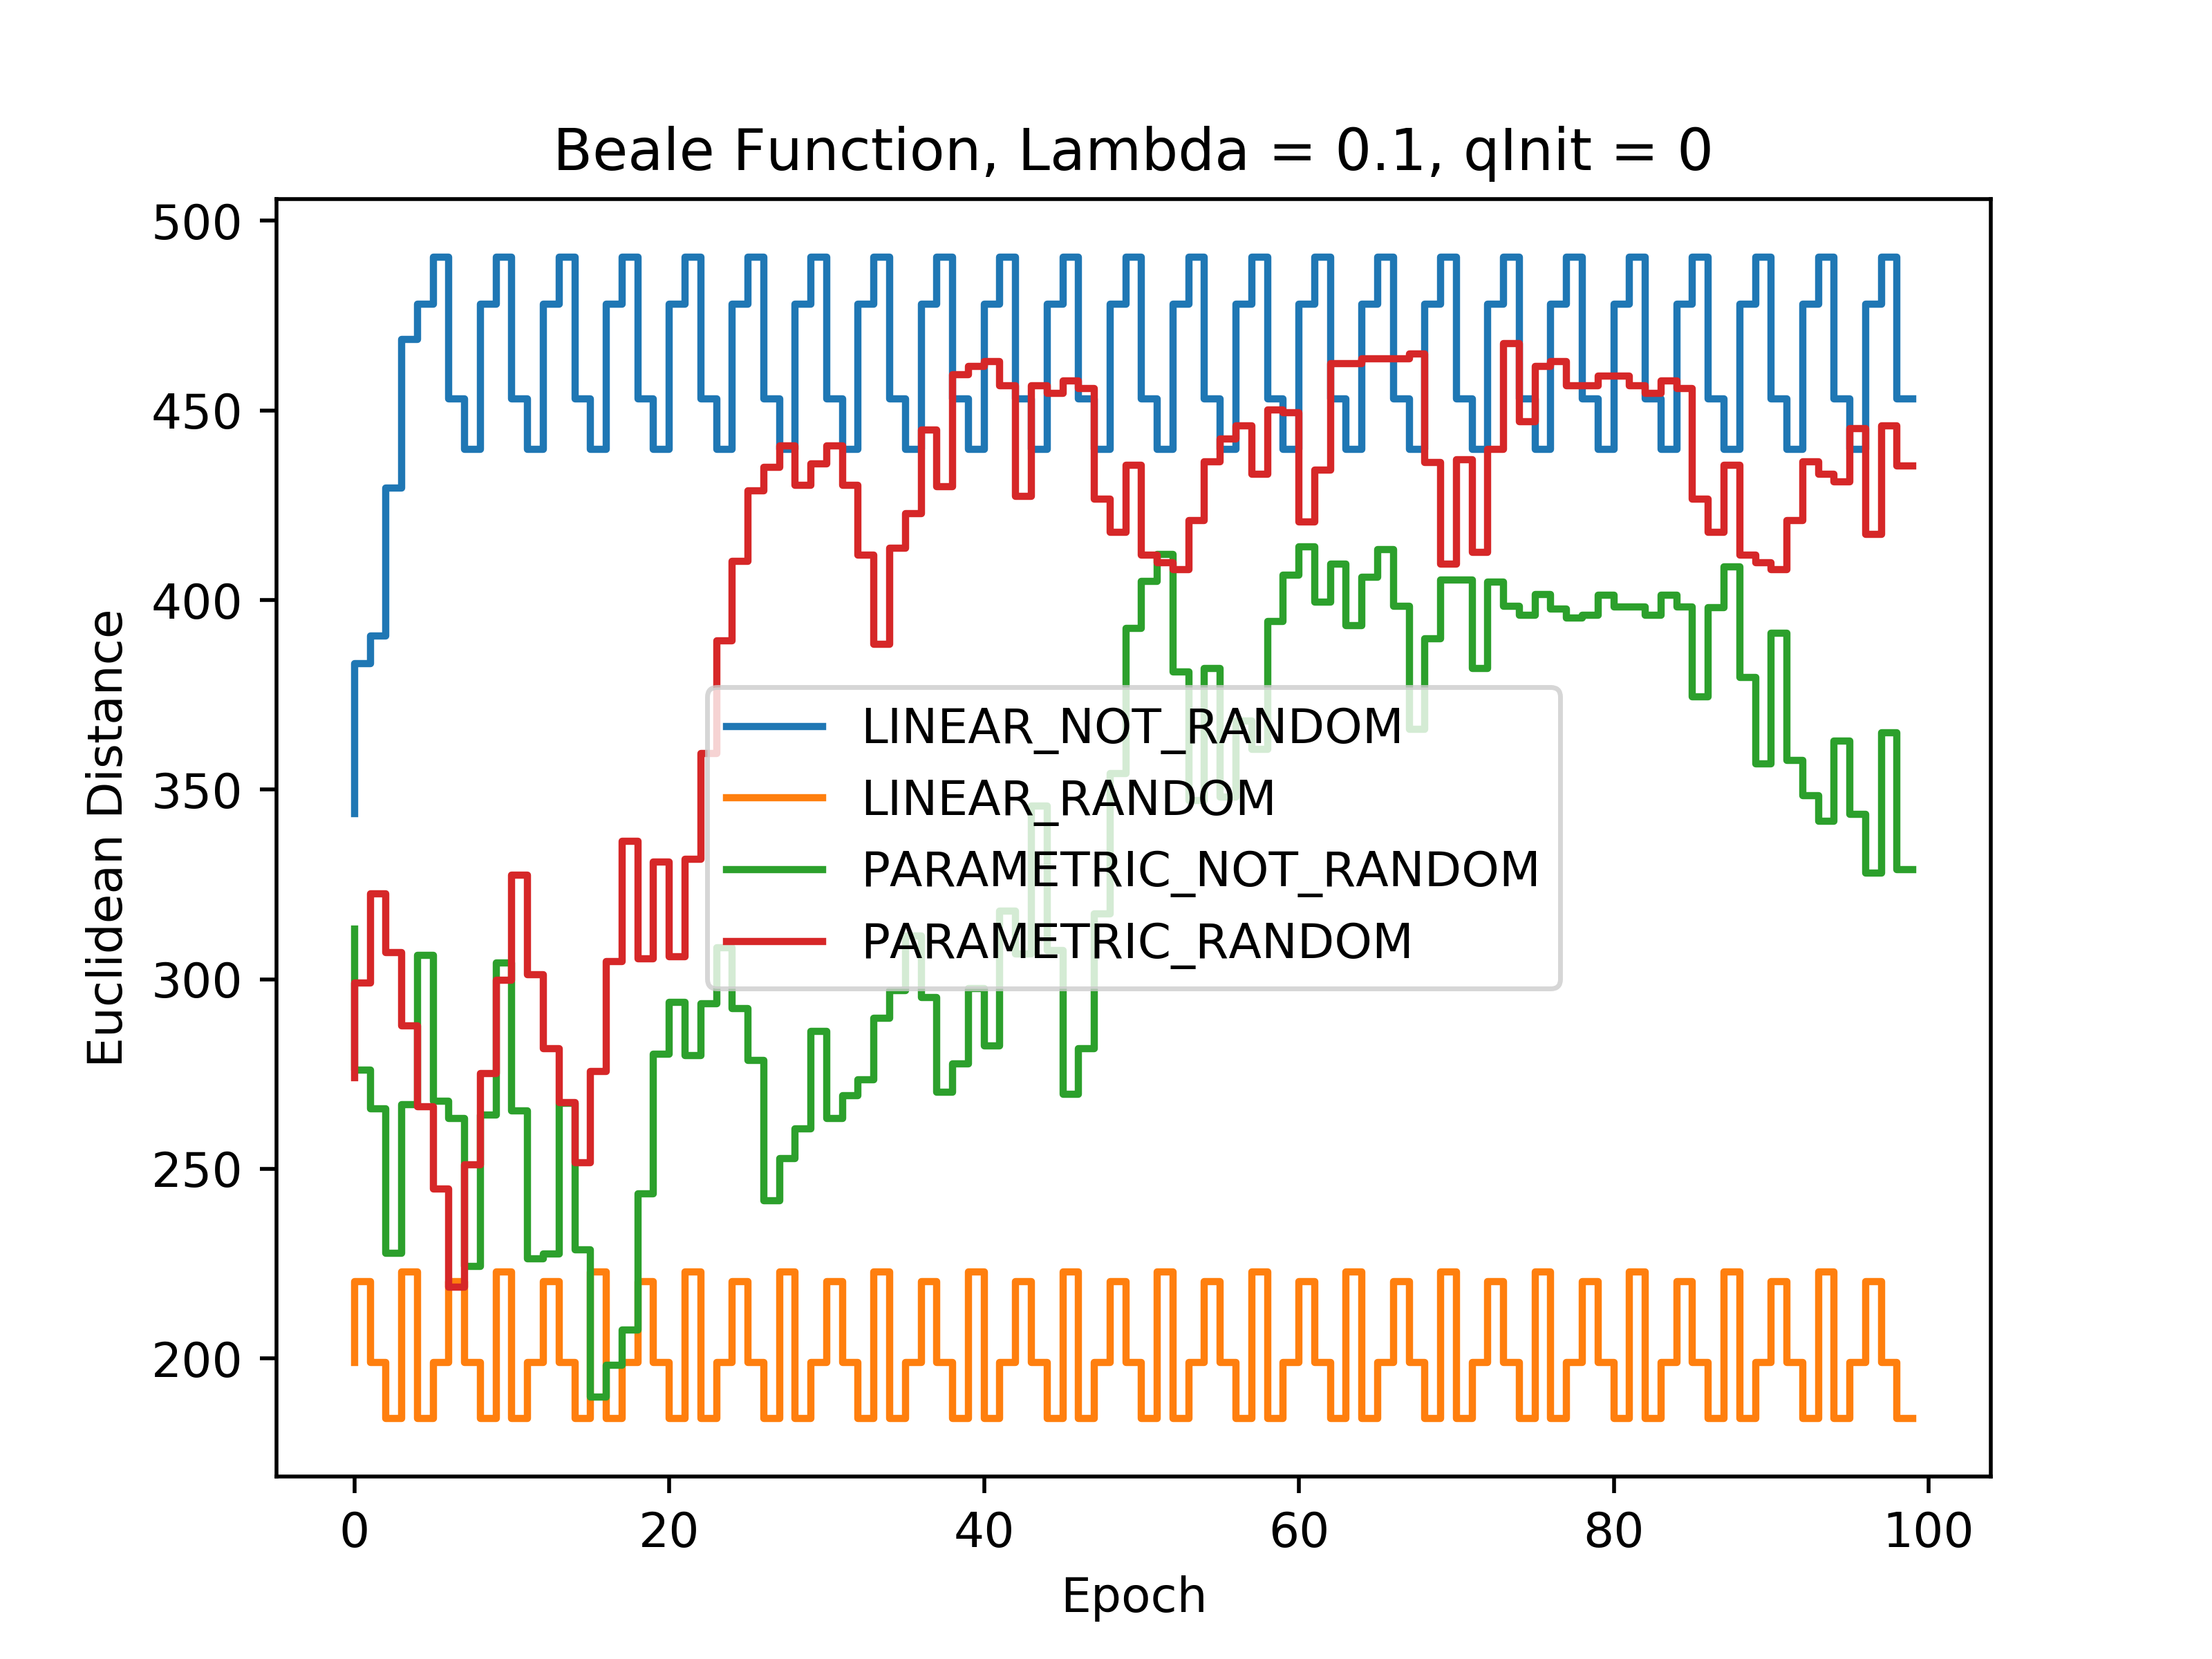
\includegraphics[width=0.4\textwidth]{BealeDifference}
		}
		\subfigure[]{%
			\label{fig:BealeValueFunction}
			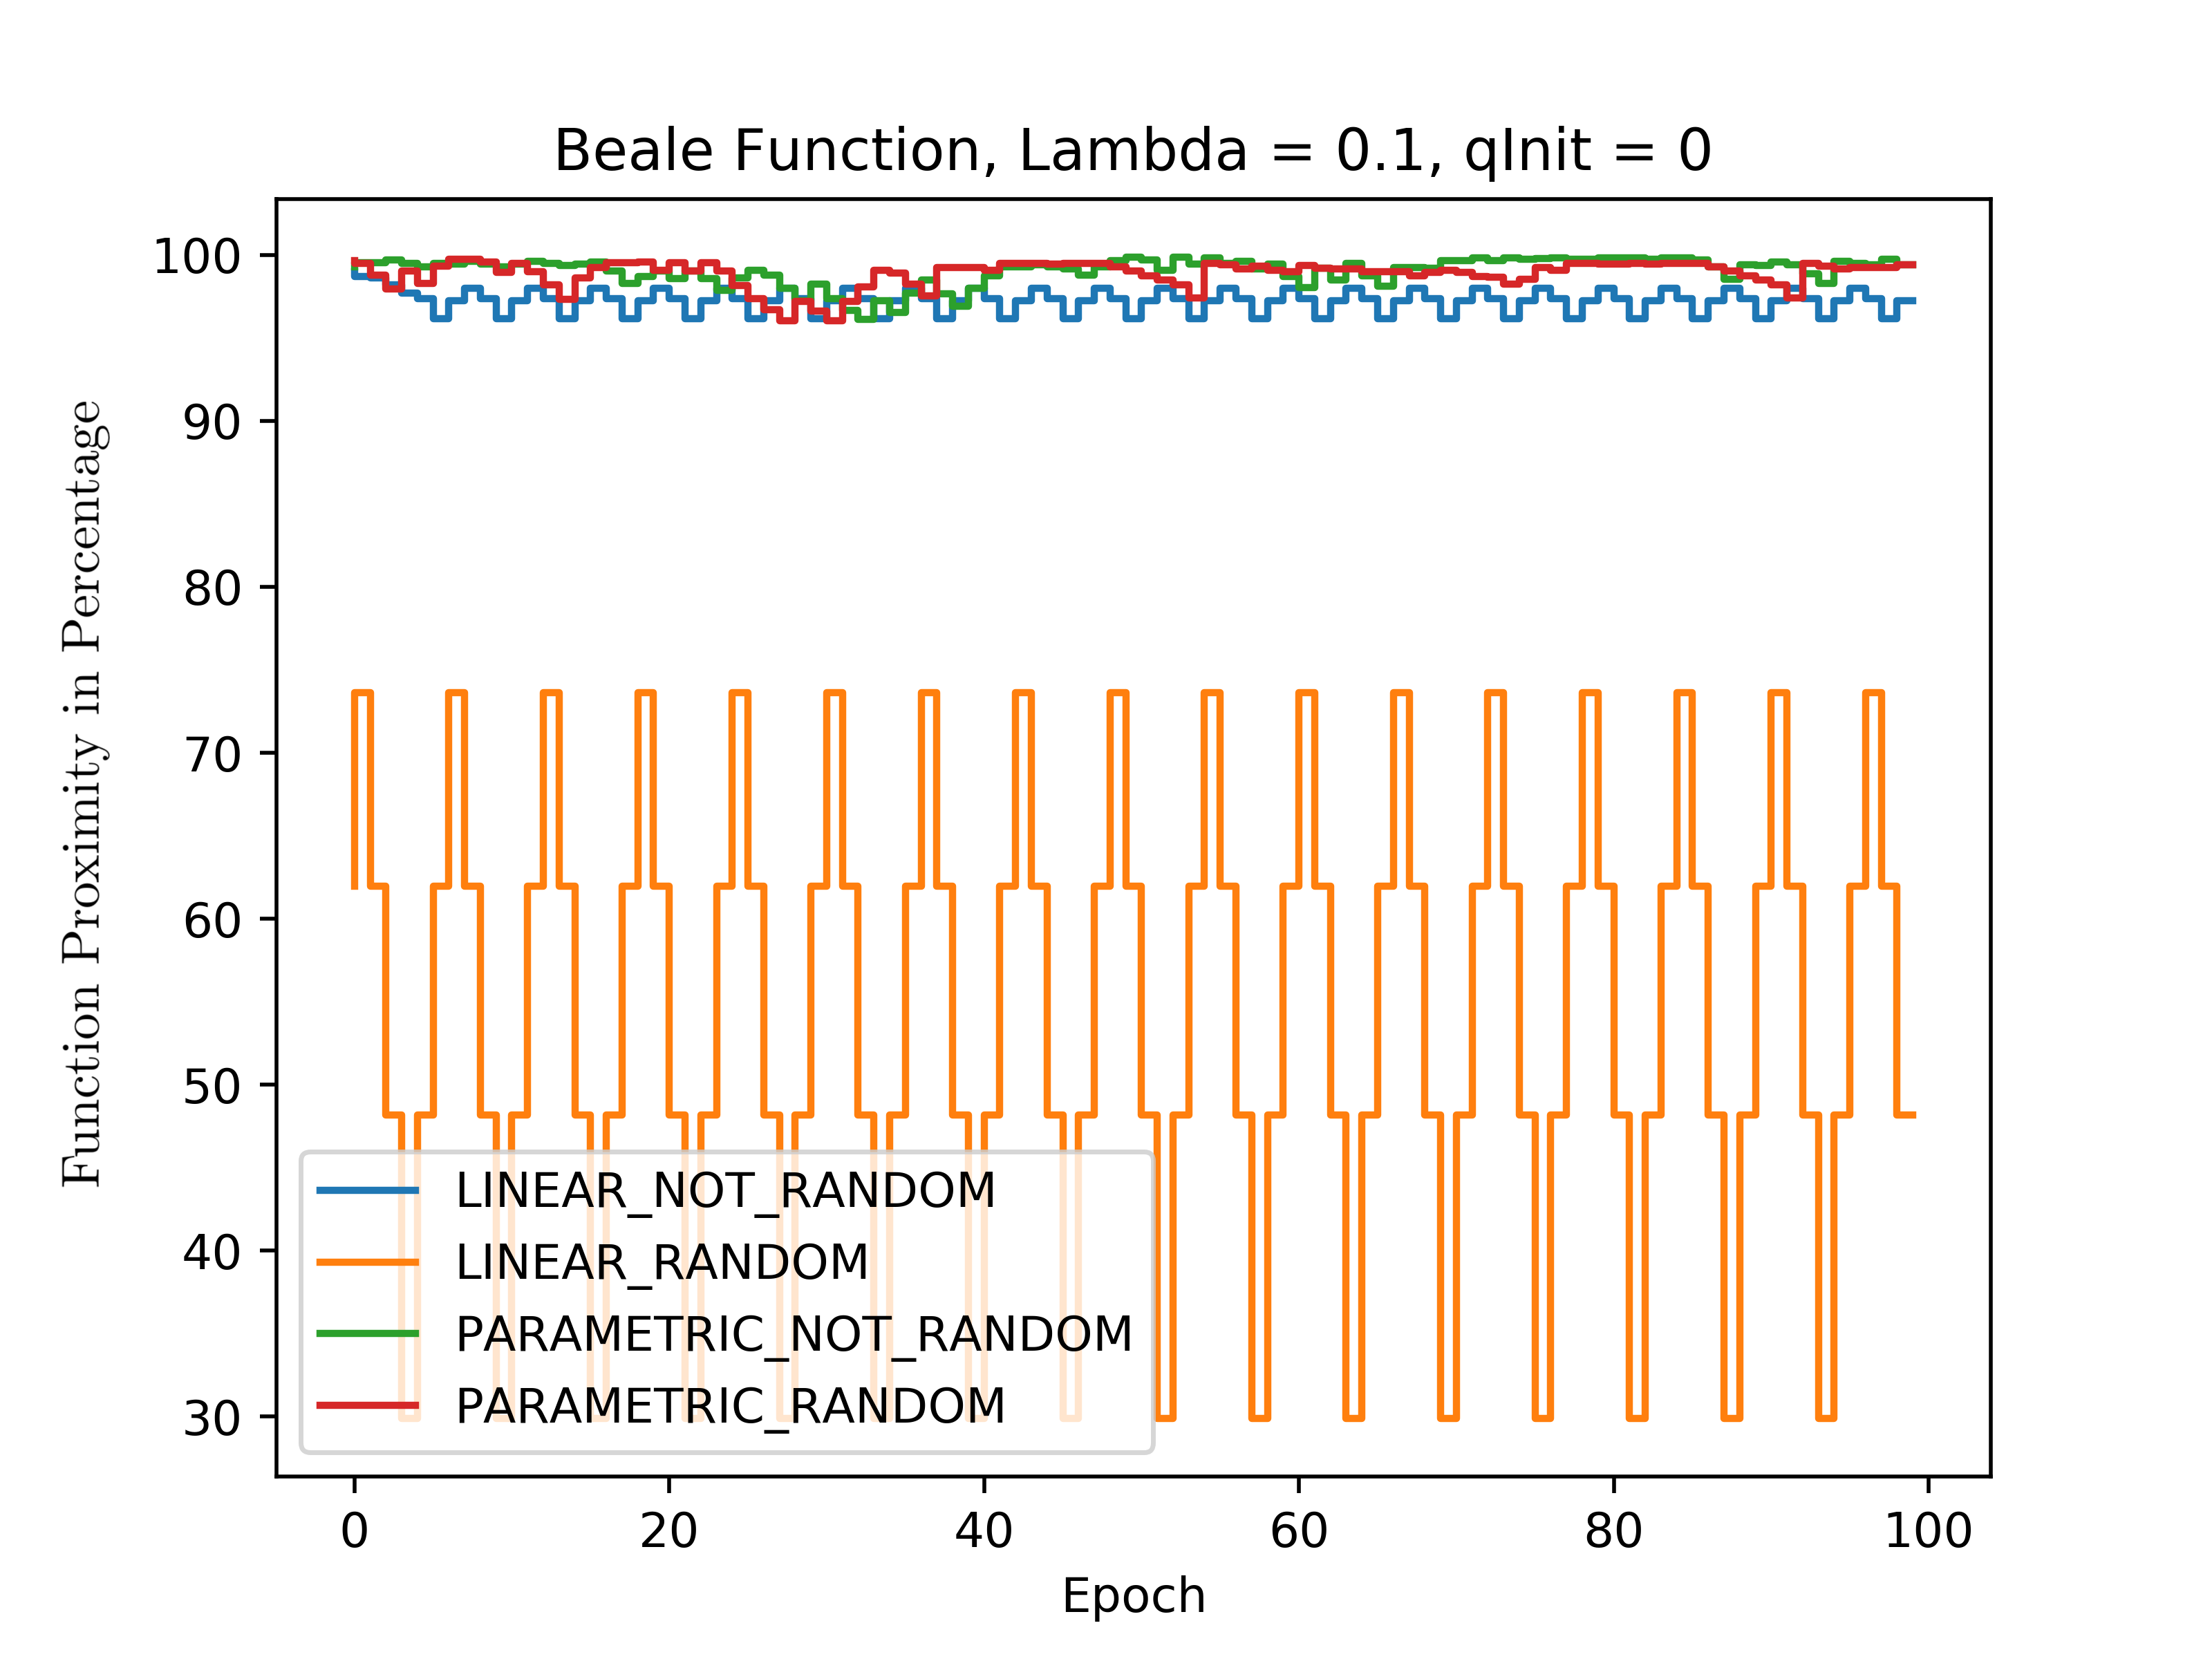
\includegraphics[width=0.4\textwidth]{BealeValueFunction}
		}\\
		\subfigure[]{%
			\label{fig:BealeGap}
			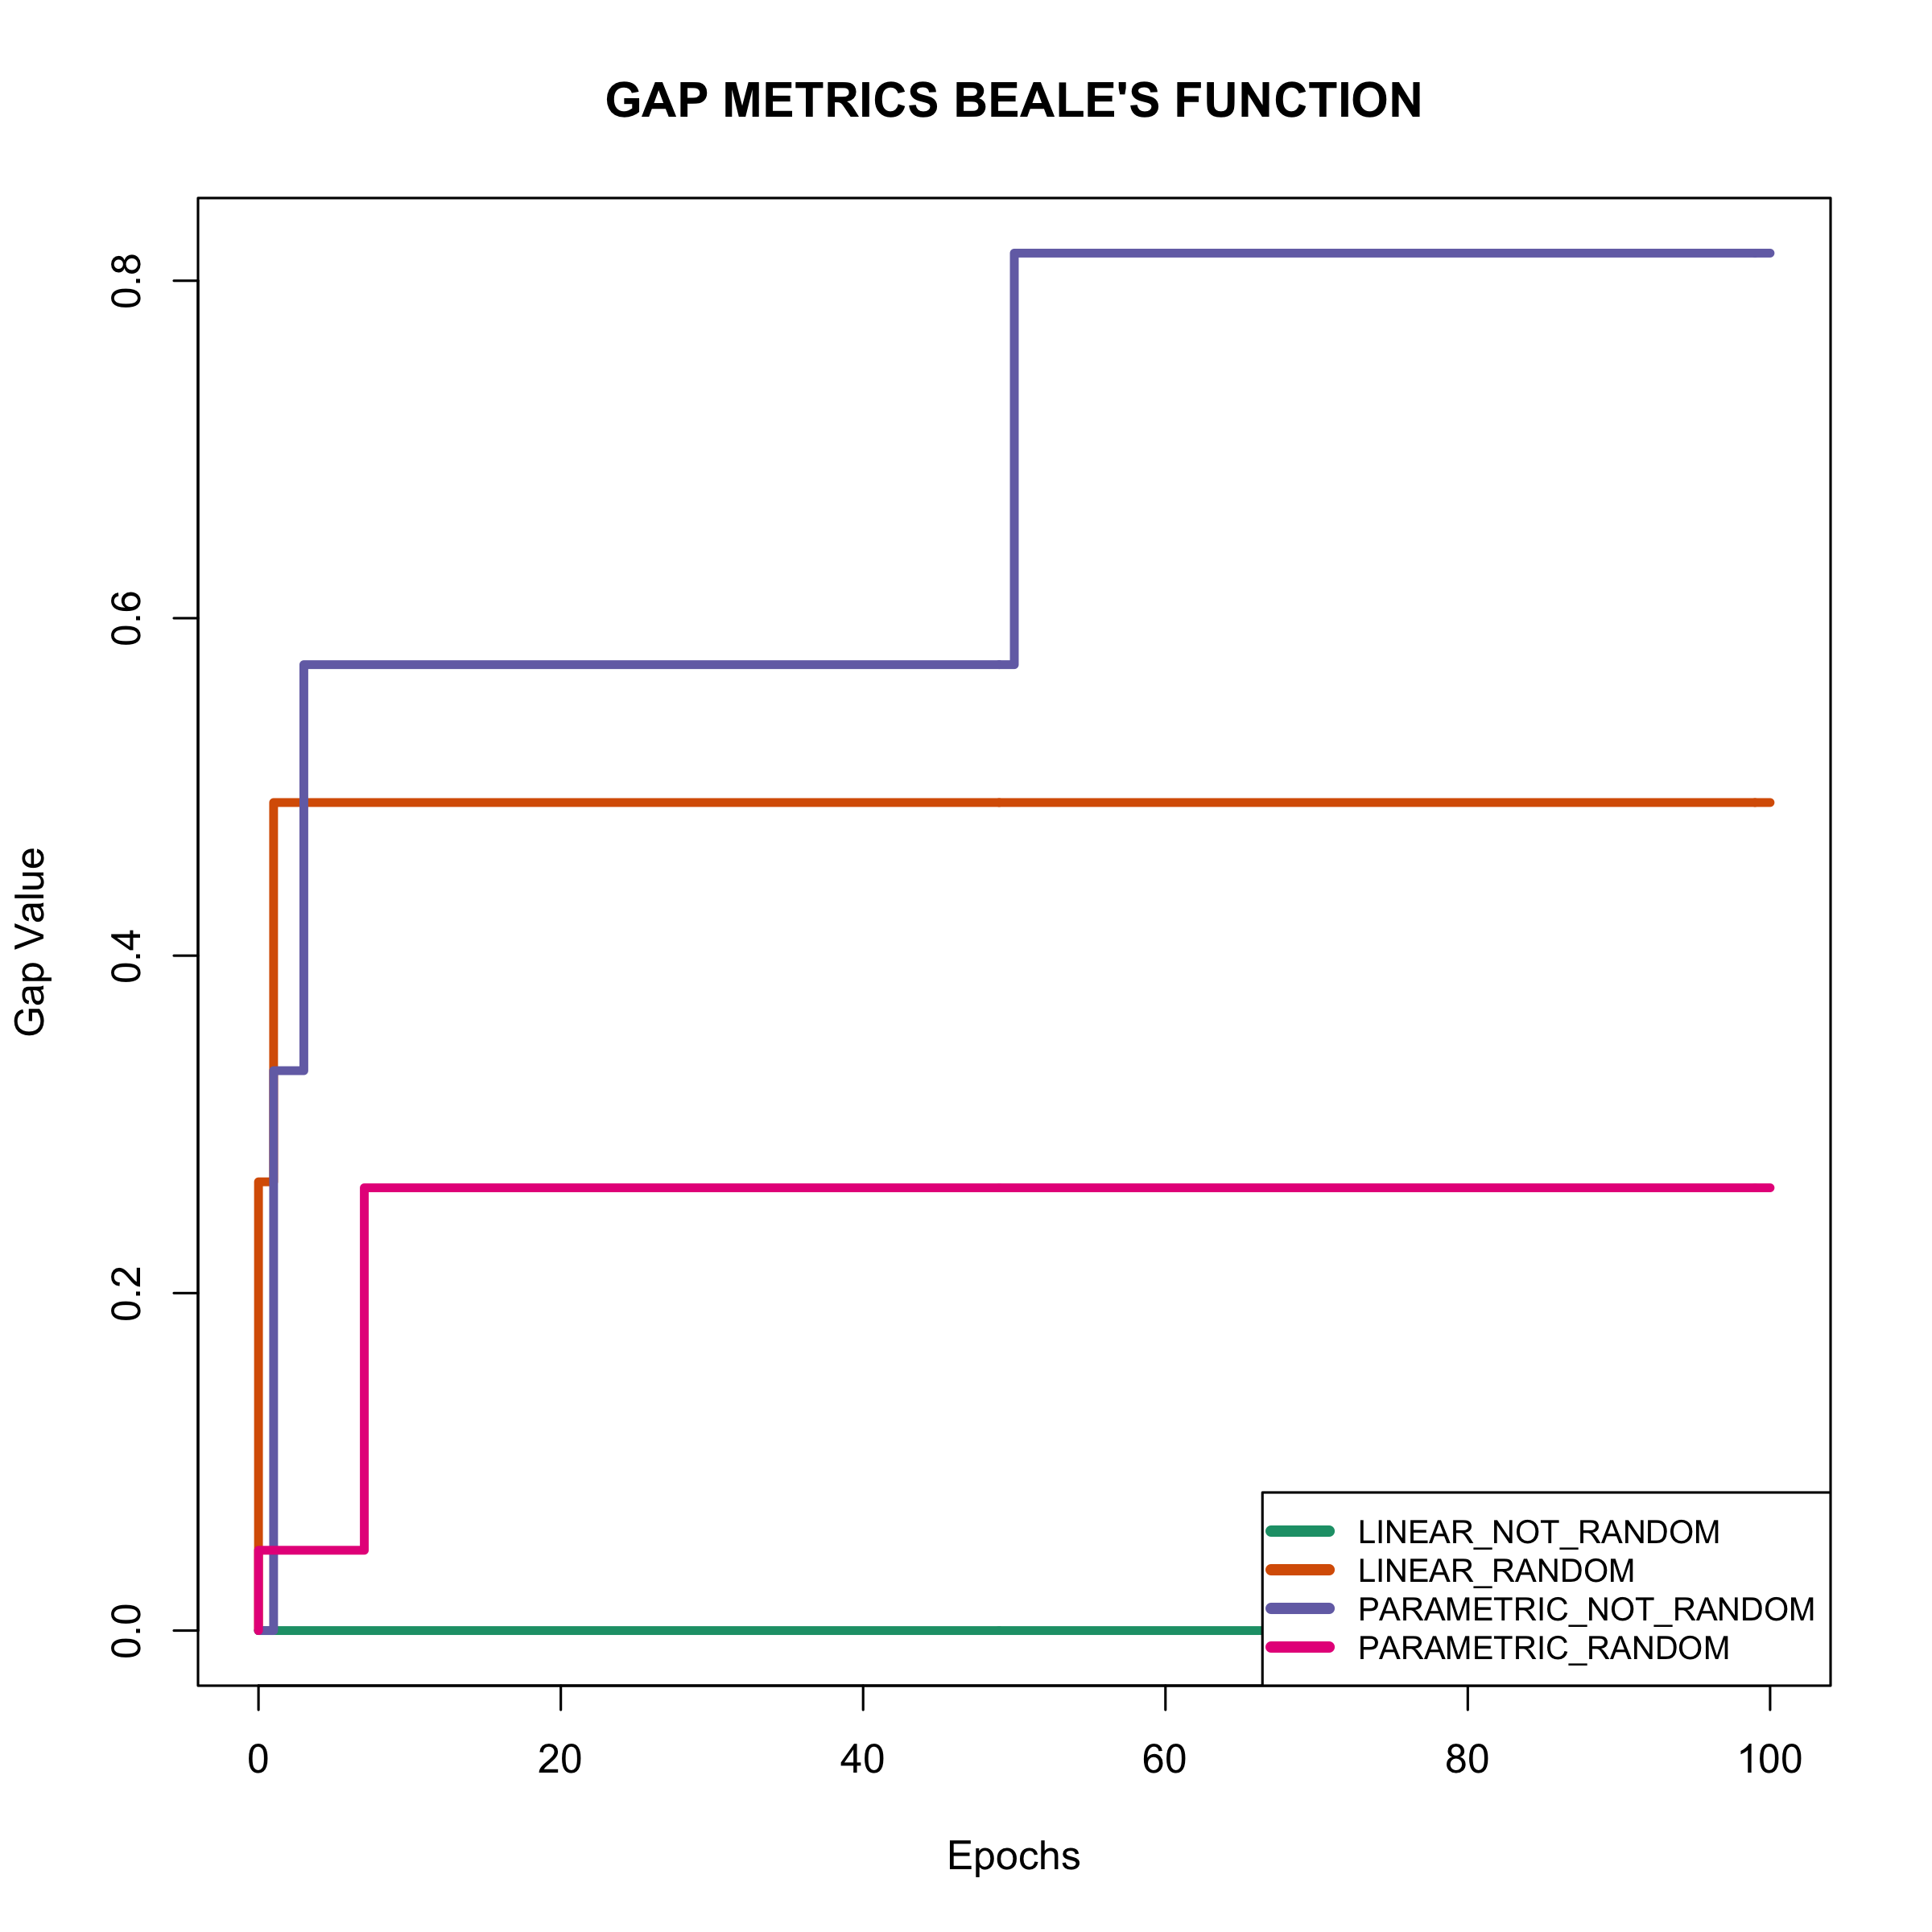
\includegraphics[width=0.4\textwidth]{BealeGap}
		} \\
		
	\end{center}
	\caption{
		Beale Function.
	}
	\label{fig:BealeResults}
\end{figure}

\subsection{Beale Function} Giving an overview to figure \ref{fig:BealeResults} it is possible to see that Beale Function represents the case in which {\tt SARSA($\lambda$)} algorithm' s declinations do worst. 

Plot (a) of figure \ref{fig:BealeResults} graphically represents performances of the four possible declinations of {\tt SARSA($\lambda$)} algorithm obtained considering the \textit{Euclidean distance metric}. Looking at the {\tt linear, not random} declination it is possible to note a growing performance' s worsening until tenth epoch. Starting from epoch ten algorithm's declination starts to stabilize developing a recurrent pattern. Using this declination, the average Euclidean distance from the maximum is $462.4$ pixels.

{\tt Linear, random} declination seems to be the one which performs better. Its average Euclidean distance from the maximum is $201.6$ pixels and its standard deviation is the lowest of the set with a value of $15.4$. This means that it has a relatively good stability. Looking at plot (a) what just said can be easily proved. The current declination starts from a point relatively near to the maximum and never departs from its developing a recurrent pattern.

Looking at {\tt parametric, not random} declination of  {\tt SARSA($\lambda$)} algorithm it is possible to note an high instability. In the very first epochs the distance between the starting point and the maximum slowly decreases, but starting from epoch thirty it starts to messily increase achieving a level near to $350$ pixels. This high instability is reflected also in the high level of standard deviation (table $5.5$).

{\tt Parametric, random} declination combines instability and inaccuracy. It starts from a distance of about $300$ pixels and messily increase its. Its performance is the worst one with an average Euclidean distance of $402.99$ pixels and a standard deviation of $66.6$ (table $5.5$).

Generally speaking it is possible to affirm that those bad performances are the result of an inadequate training space and of a particularly flat function's shape. In addition to this, as already explained, parametric declinations do worst than corresponding ones because of the reduced amount of movement at each epoch. The relatively better performance of {\tt linear, random} declination depends on the possibility to select a starting point closer to the maximum. \\

\begin{table}[h!]
\centering
\resizebox{\linewidth}{!} {
	\begin{tabular}{c| cccccc} 
		\hline \textbf{Beale Function}
		& \textbf{Mean (pixels)} & \textbf{Standard deviation} \\ 
		\hline Linear not Random
		& $462.4$ & $25.7$\\ 
		\hline Linear Random
		& \cellcolor{red!25}$201.6$ & \cellcolor{red!25}$15.4$\\ 
		\hline Parametric not Random
		& $329.8$ & $62.7$\\ 
		\hline Parametric Random
		& $402.99$ & $66.6$ \\ 
		\hline 
	\end{tabular} 
}
\label{BealeTabEuclidean}
\caption{Euclidean Metric's Performances}
\end{table}

Looking at plot (b) of figure \ref{fig:BealeResults} it is possible to note an inconsistency with what said until now. Only {\tt linear, random} configuration makes an highly swinging performance varying between a percentage of value function' s proximity of about $75\%$ to a percentage of $30\%$. All other declinations make performances around $100\%$ of value function' s proximity. Even looking at table $5.6$ this impression is proved by the high standard deviation of {\tt linear, random} configuration and by the high average of value function' s proximity of all other declinations. These apparently good performances depends on the function' s shape that is very flat. 

\begin{table}[h!]
	\centering
	\resizebox{\linewidth}{!} {
		\begin{tabular}{c| cccccc} 
			\hline \textbf{Beale Function}
			& \textbf{Mean (\%)} & \textbf{Standard deviation} \\ 
			\hline Linear not Random
			& $97.25$ & \cellcolor{green!25}$0.70$\\ 
			\hline Linear Random
			& $54.26$ & $13.89$\\ 
			\hline Parametric not Random
			& \cellcolor{green!25}$99.06$ & $0.81$ \\ 
			\hline Parametric Random
			& $98.88$ & $0.798$ \\ 
			\hline 
		\end{tabular} 
}
	\caption{Function Proximity in Percentage.} 
	\label{BealeTabProximity}
\end{table}

Deception can also be revealed by observing plot (c) of figure \ref{fig:BealeResults}. The relatively best performing declination is the {\tt parametric, not random} one which achieves an effectiveness in finding the maximum of about $0.8$ out of $1.0$. It is also proved by table $5.9$. {\tt Parametric, not random} declination achieves point $(-0.77, 1.5599)$ with a value function of $1997.392$ out of $2000$. The worst performing one is the {\tt linear, not random} declination with a constant \textit{Gap value} equals to $0$.

\begin{figure}[h!]
	\begin{center}
		\subfigure[]{%
			\label{fig:StyblinskiDifference}
			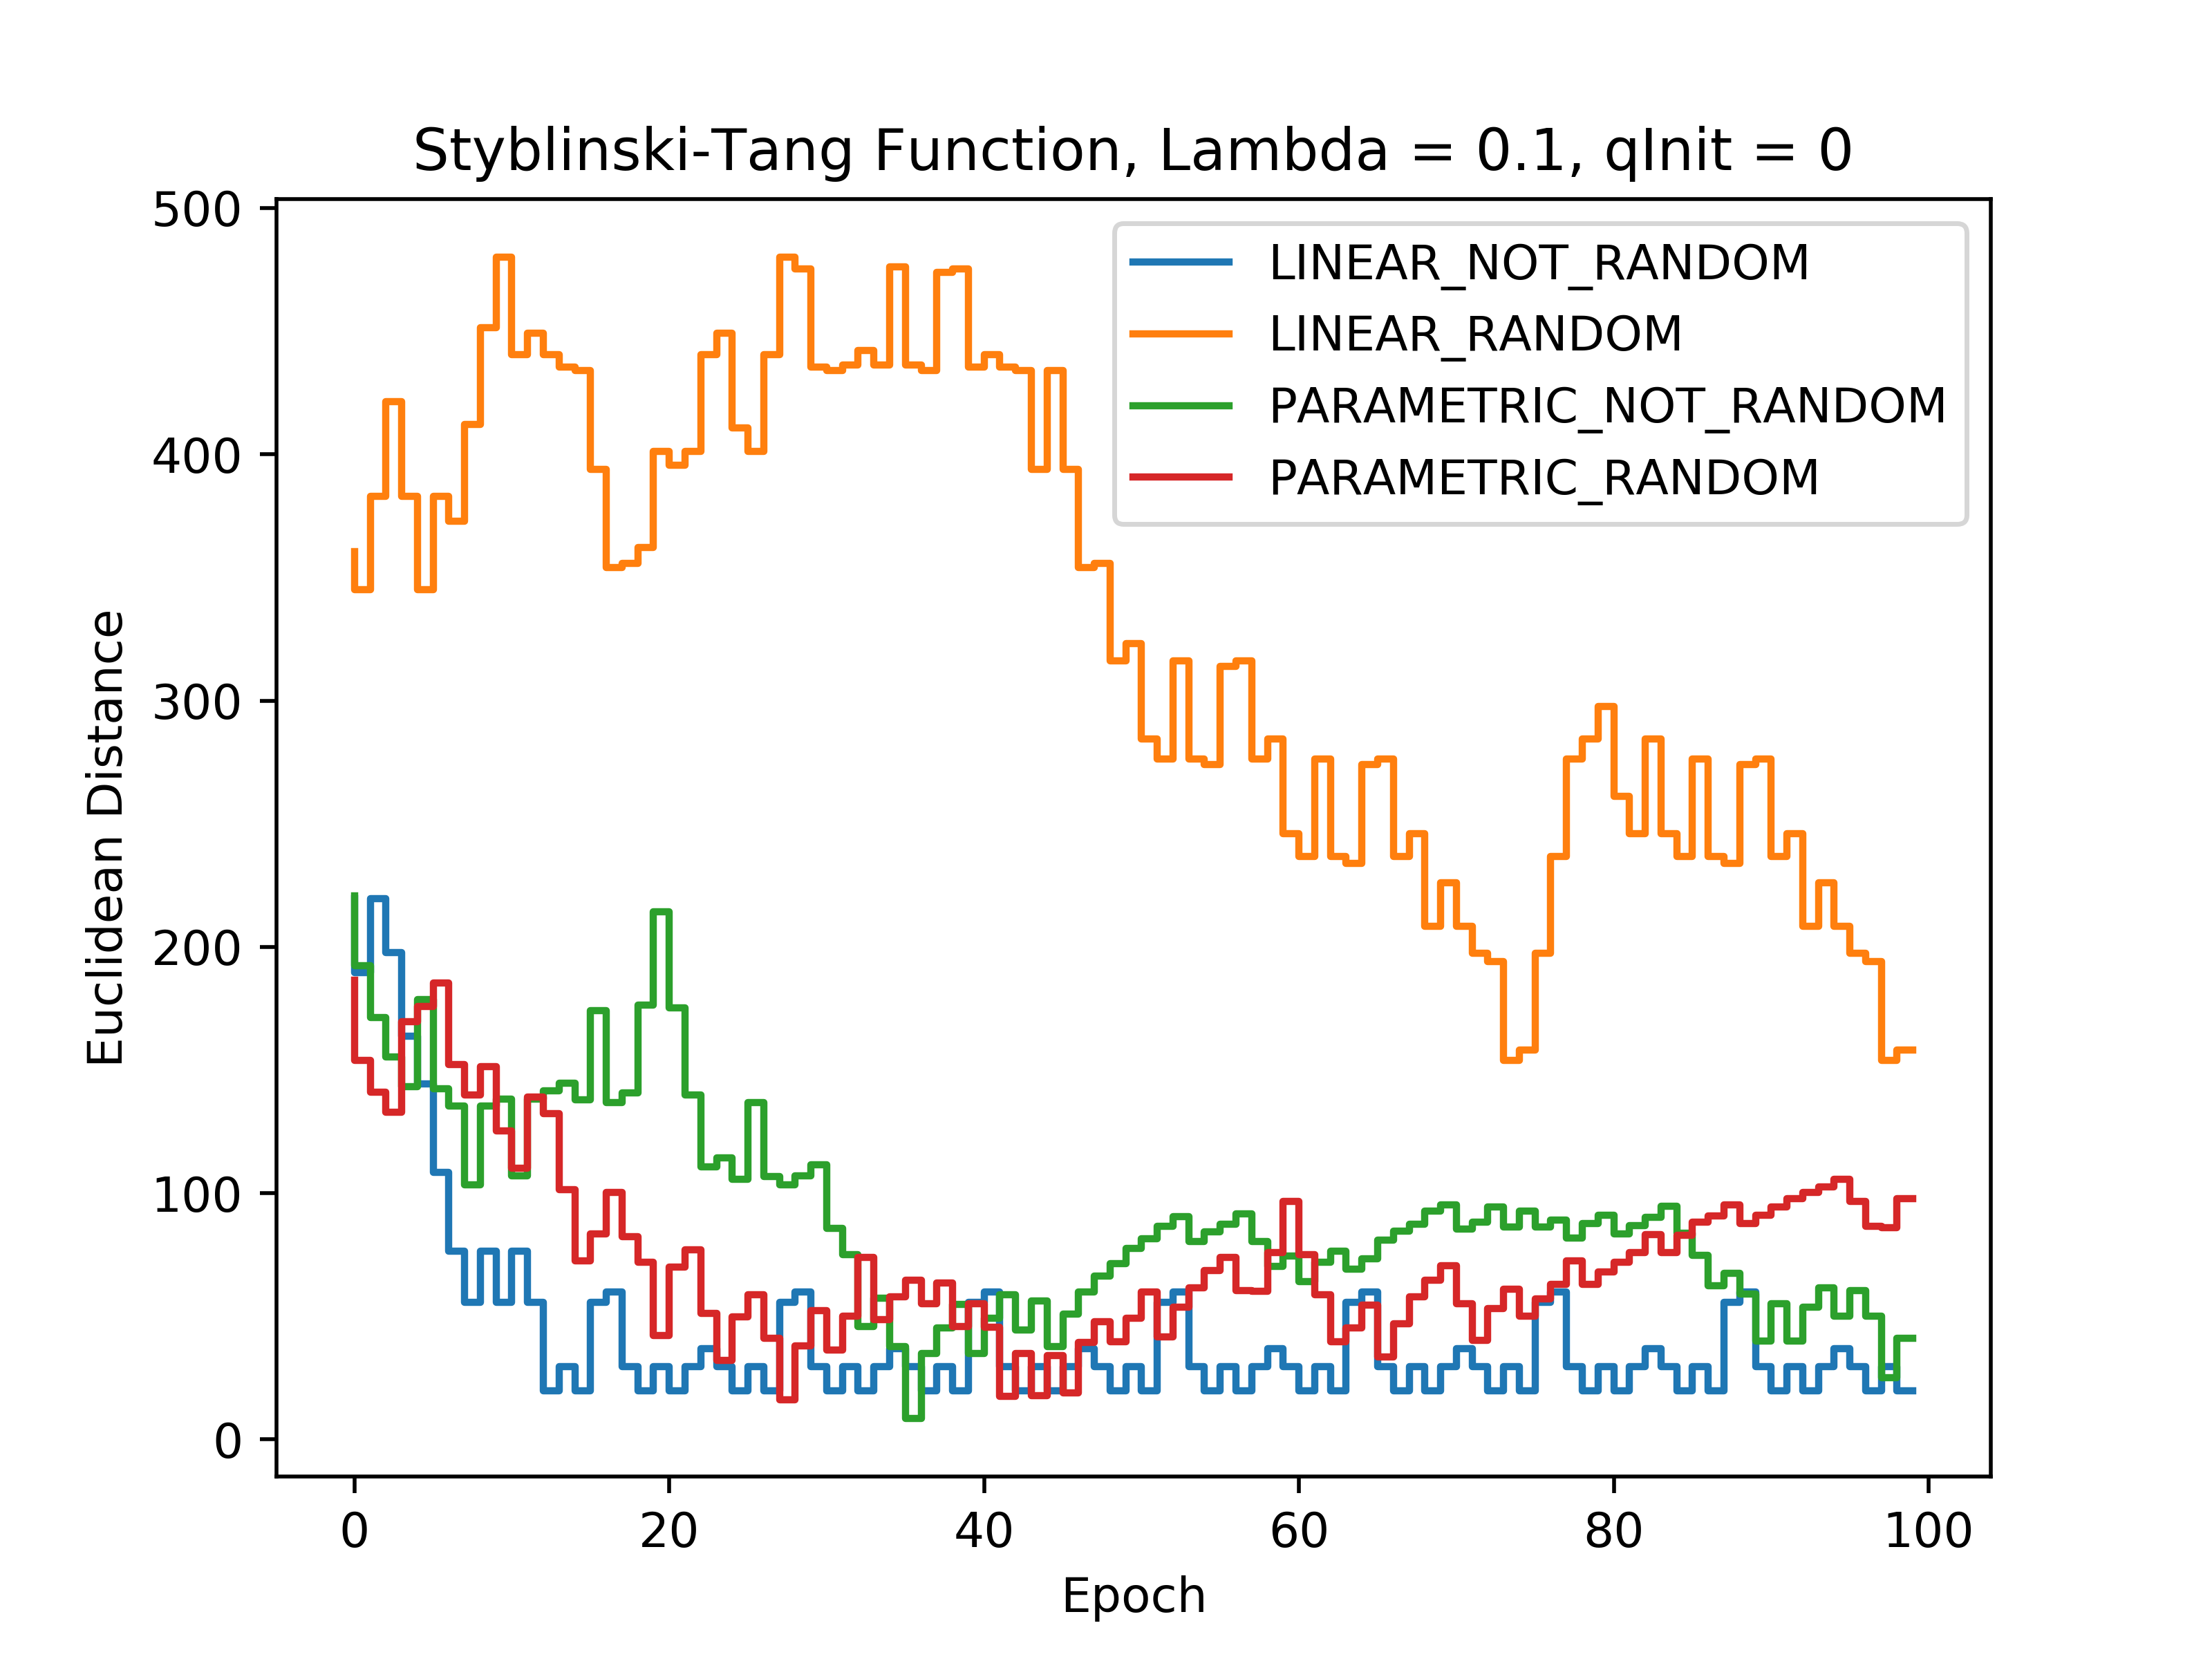
\includegraphics[width=0.4\textwidth]{StyblinskiDifference}
		}
		\subfigure[]{%
			\label{fig:StyblinskiValueFunction}
			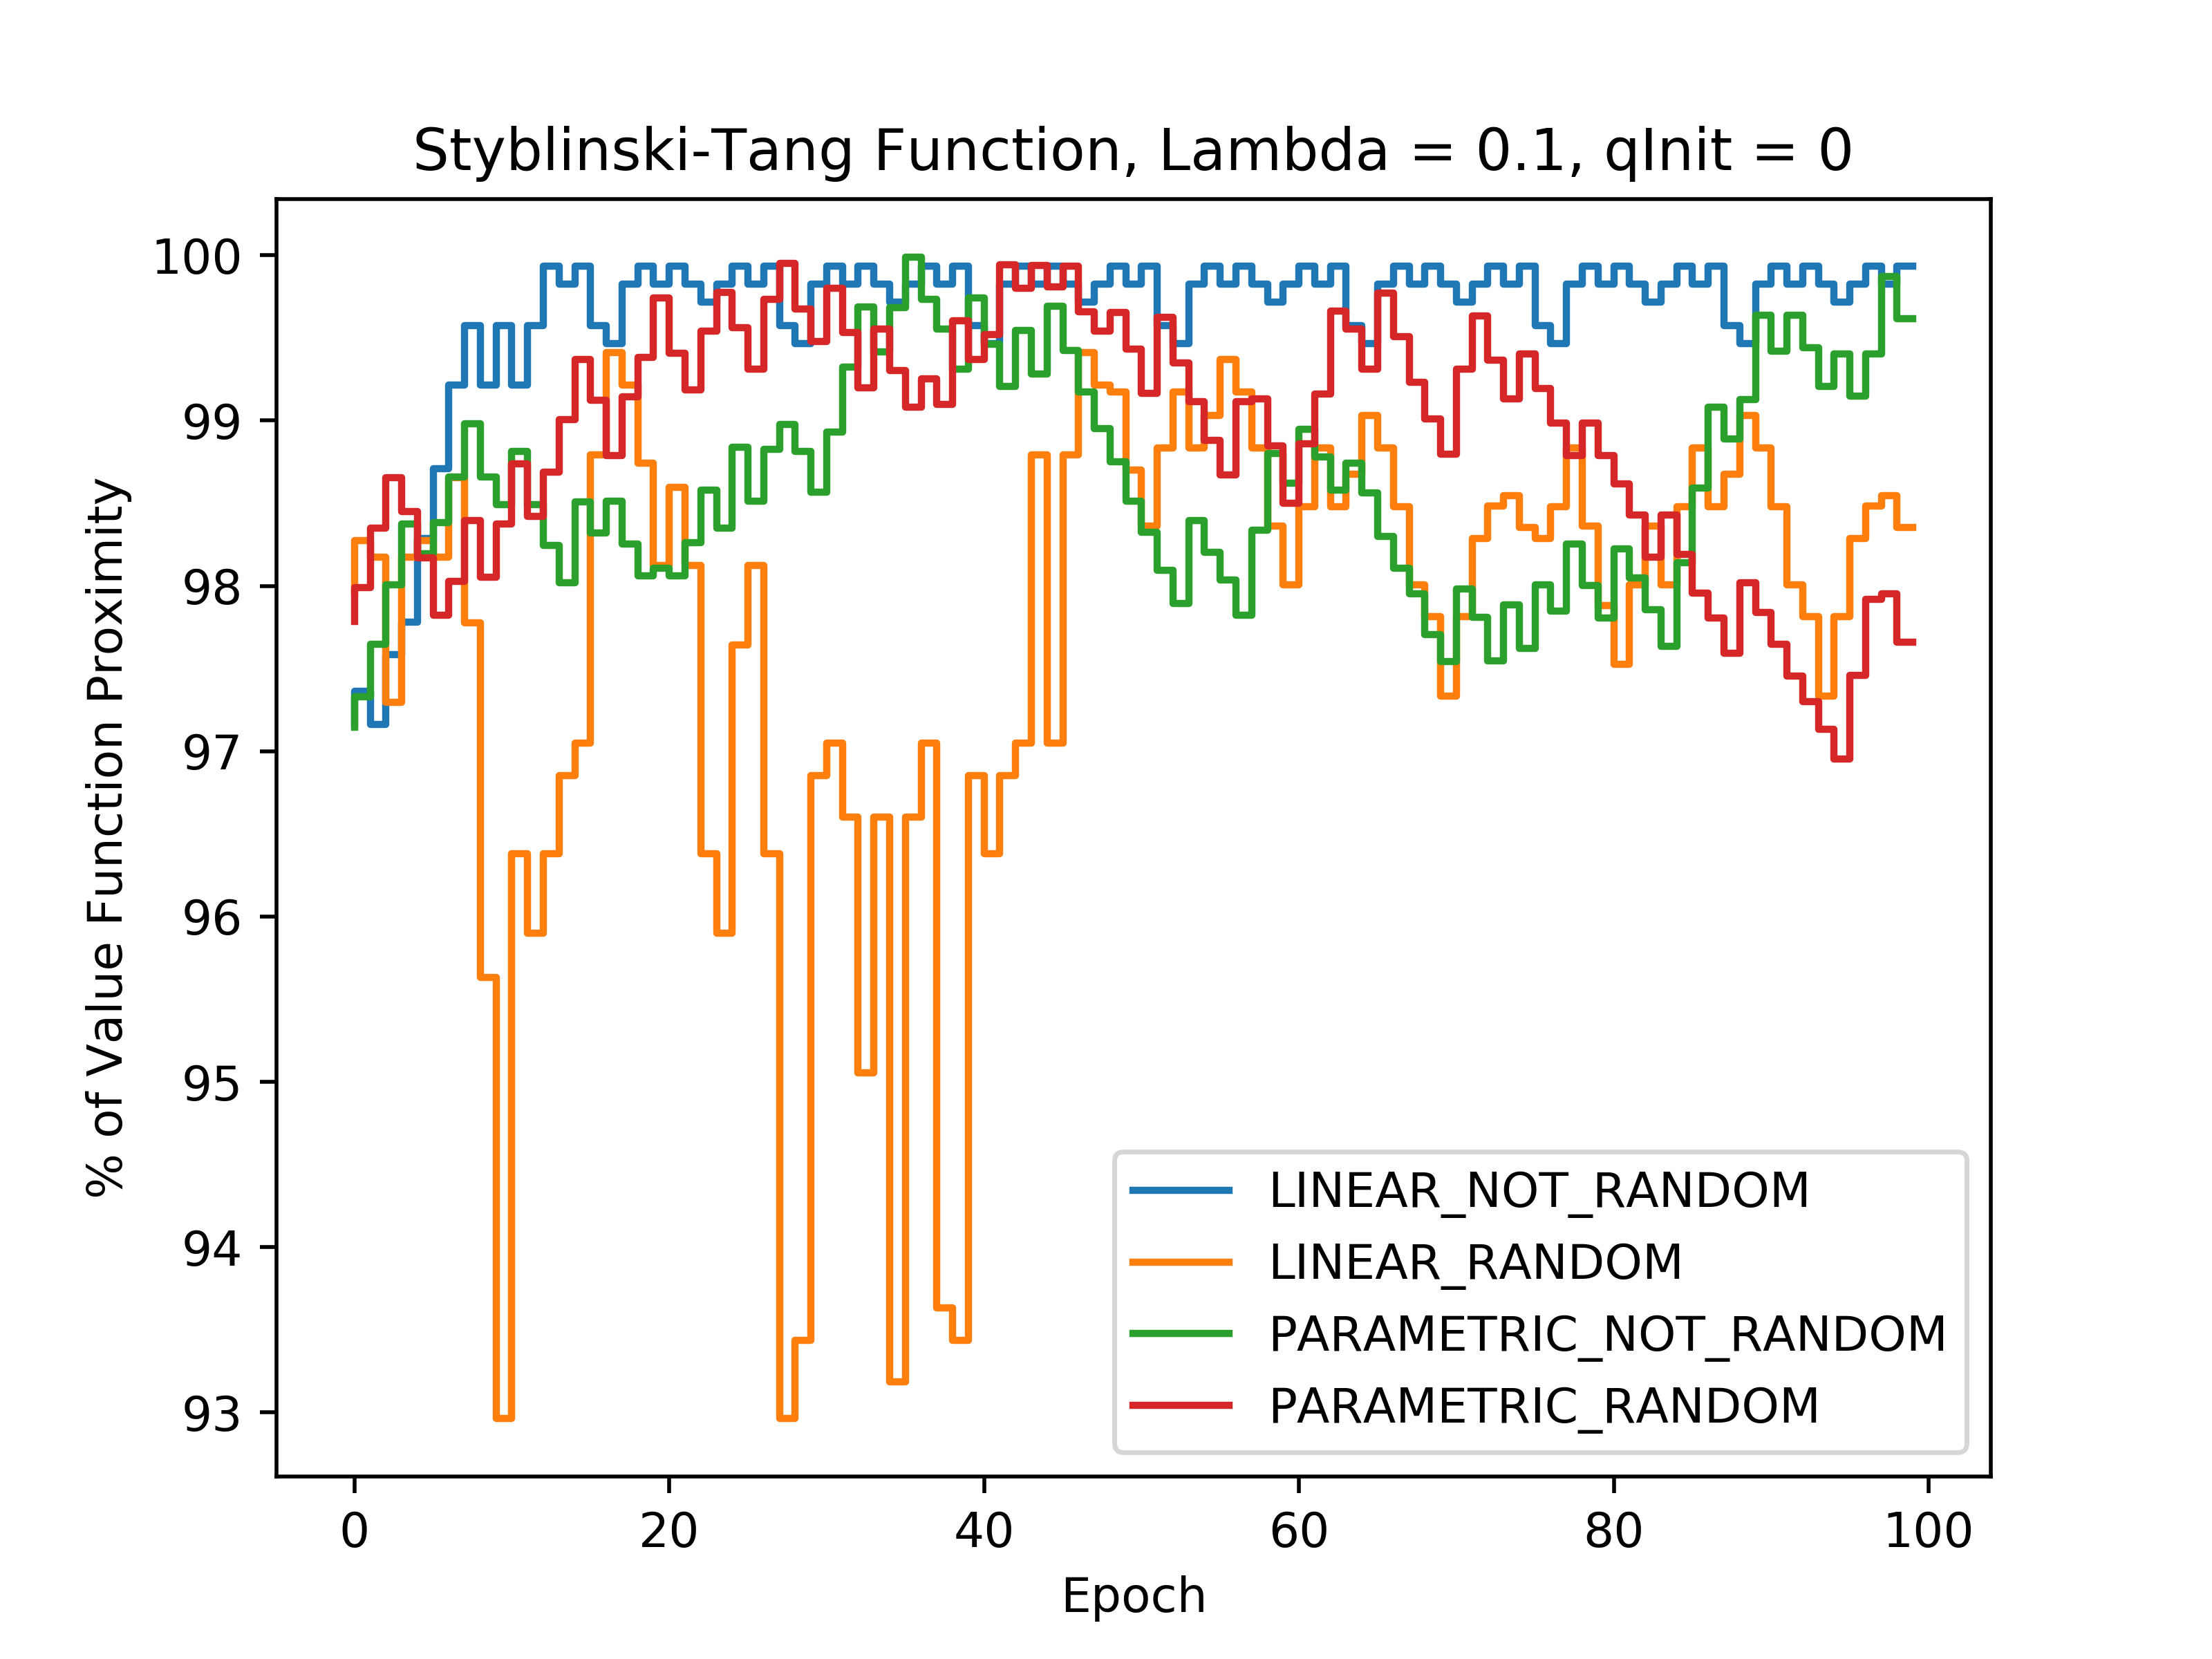
\includegraphics[width=0.4\textwidth]{StyblinskiValueFunction}
		}\\
		\subfigure[]{%
			\label{fig:StyblinskiGap}
			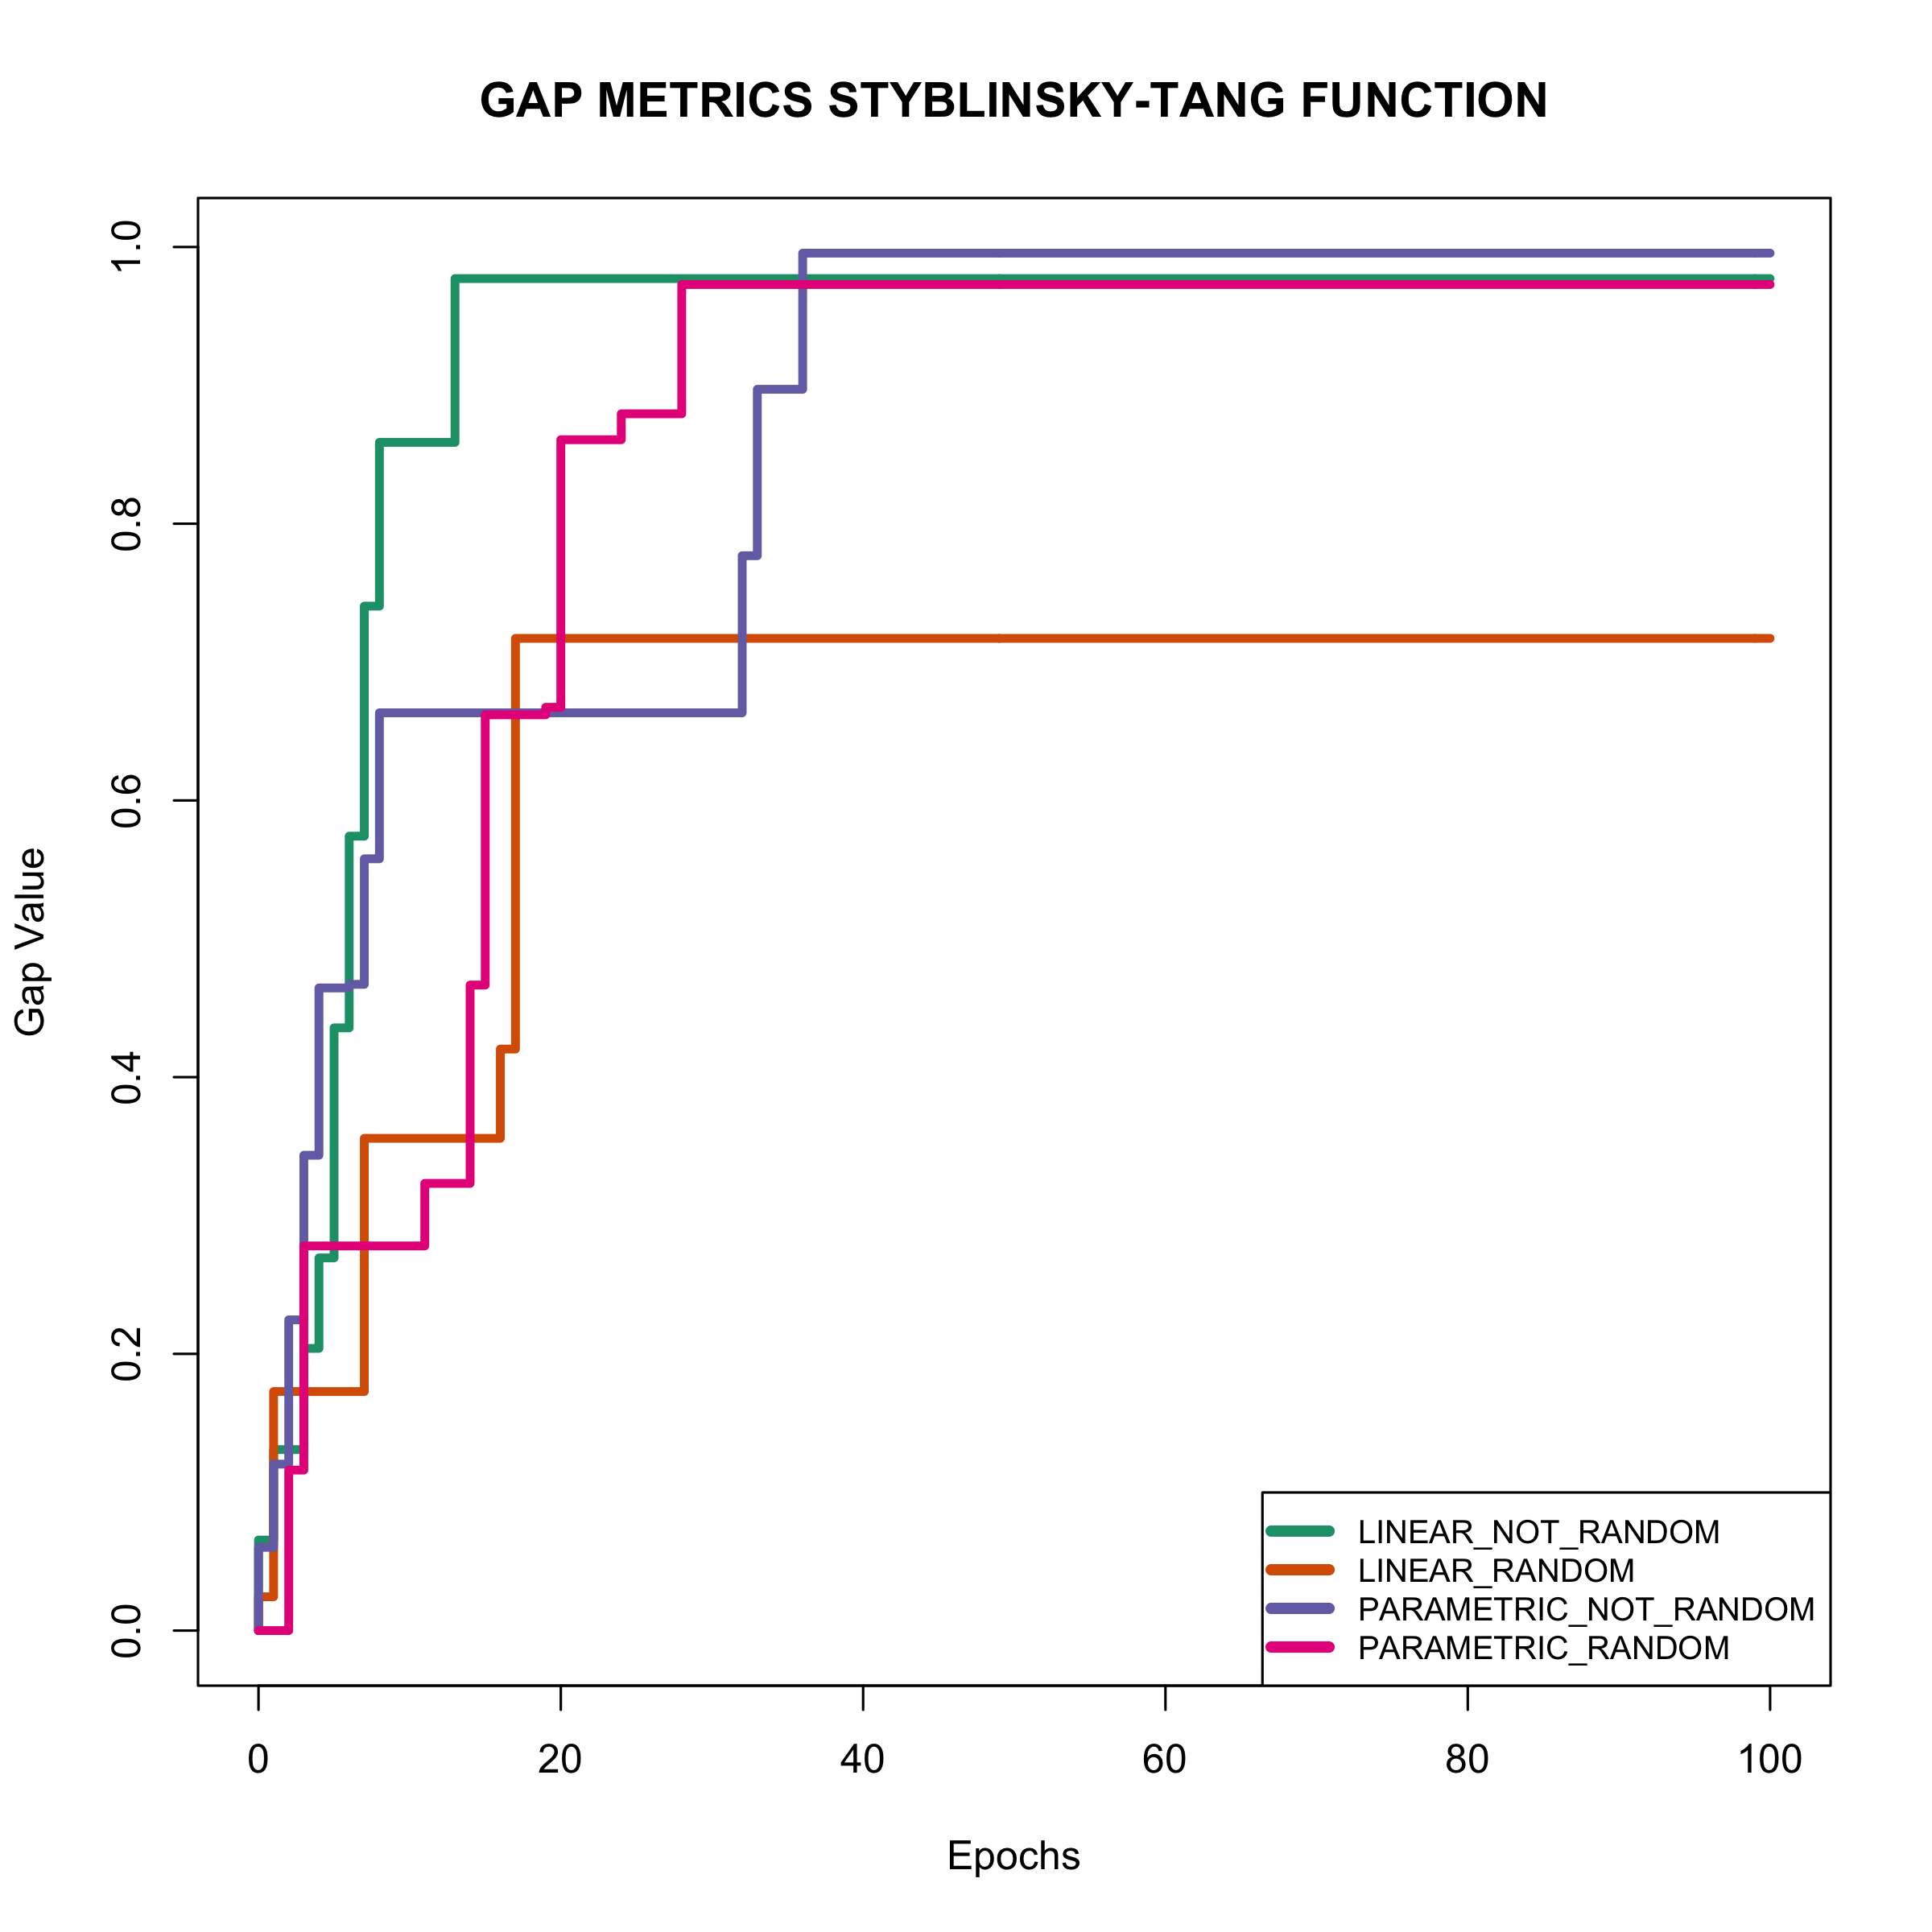
\includegraphics[width=0.4\textwidth]{StyblinskiGap}
		} \\
		
	\end{center}
	\caption{
		Styblinski Function.
	}
	\label{fig:StyblinskiResults}
\end{figure}

\subsection{Styblinski-Tang' s Revised Function} Plot (a) of figure \ref{fig:StyblinskiResults} graphically represents performances of the four possible declinations of {\tt SARSA($\lambda$)} algorithm obtained considering the \textit{Euclidean distance metric}. 

Looking at the {\tt linear, not random} declination's performance, the Euclidean difference between the agent's position and the global maximum is about $200$ pixels. Staring from the twentieth epoch it starts to stabilize around an Euclidean distance level from the maximum of about $40$ pixels. Note that in less than twenty epochs the Euclidean distance from the maximum is about the $20\%$ of the starting one. The current declination also reveals a great stability. With an average Euclidean distance of $43.63$ pixels and a standard deviation of $41.05$, the {\tt linear, not random} declination is the best of the set (table $5.7$).

A decisively worse performance is given by the {\tt linear, random} declination. It starts with an Euclidean distance from the maximum of about $360$ pixels and messily decreases until achieving a level of $180$ pixels. The noise just described is also proved by the highest average Euclidean distance and by the highest standard deviation of the set (table $5.7$).

Last two, parametric declinations give for the first time the possibility to really see behaviour of parametric declination. Starting from about the fiftieth epoch, {\tt parametric, not random} movement starts to imperceptibly increase. This lower amount of movement compared to the non parametric movements depends on the definition of the parametric movement itself. The same behaviour can be seen in {\tt parametric, random} declination starting from epoch $75$. This declination performs better then the {\tt parametric, not random} one in the first epochs but it performs worse in the last ones. With an average Euclidean distance from the maximum of $75.26$ pixels, and with an average standard deviation of $37.34$, the {\tt parametric, random} declinations is generally better than the {\tt parametric, not random} one.

\begin{table}[h!]
	\centering
	\resizebox{\linewidth}{!} {
		\begin{tabular}{c| cccccc} 
			\hline \textbf{Styblinski-Tang Function}
			& \textbf{Mean (pixels)} & \textbf{Standard deviation} \\ 
			\hline Linear not Random
			& \cellcolor{red!25}$43.63$ & \cellcolor{red!25}$41.05$\\ 
			\hline Linear Random
			& $330.16$ & $95.39$ \\ 
			\hline Parametric not Random
			& $91.79$ & $42.24$\\ 
			\hline Parametric Random
			& $75.26$ & $37.34$\\ 
			\hline 
		\end{tabular} 
	}
	\label{StyblinskiTabEuclidean}
	\caption{Euclidean Metric's Performances}
\end{table}

The performance just described is also proved by the percentage of value function' s proximity to the maximum. With an average mean of $99.63\%$ of precision, and a standard deviation of $0.57$, the {\tt linear, not random} declination is the best of the set. General good performances are also made by all other declinations except for the {\tt linear, random} one. Looking at plot (b) of figure \ref{fig:StyblinskiResults} it is possible to note an high instability of this last declination especially until epoch fifty. It than starts to stabilize varying between a proximity level of $97\%$ and $99\%$.

\begin{table}[h!]
	\centering
	\resizebox{\linewidth}{!} {
		\begin{tabular}{c| cccccc} 
			\hline \textbf{Styblinski-Tang Function}
			& \textbf{Mean (\%)} & \textbf{Standard deviation}\\ 
			\hline Linear not Random
			& \cellcolor{green!25}$99.63$ & \cellcolor{green!25}$0.57$ \\ 
			\hline Linear Random
			& $97.73$ & $1.46$ \\ 
			\hline Parametric not Random
			& $98.61$ & $0.66$\\ 
			\hline Parametric Random
			& $98.90$ & $0.74$\\ 
			\hline 
		\end{tabular} 
	}
	\label{StyblinskiTabProximity}
	\caption{Function Proximity in Percentage.} 
\end{table}

Looking at the third plot of figure \ref{fig:StyblinskiResults}, it is possible to note that the best performance is the one of the {\tt parametric, not random} declination. This result obviously depends on the fact that around the thirty-ninth epoch it reaches the maximum for then decisively distance itself from it. This behaviour is again due to the absence of an adequate training space. This lack prevents the agent from developing an optimal policy.

\begin{sidewaystable} 
	\centering
	\label{table:BestSoundings}
	\caption{Best Soundings}
	\begin{tabular}
		{l l l l l} \hline Name & Linear Not Random & Linear Random & Parametric Not Random & Parametric Random \\
		\hline Himmelblau & \vtop{\hbox{\strut $2486.938$}\hbox{\strut $(2.67, 1.34)$}\hbox{\strut}\hbox{\strut}} &\cellcolor{blue!25} \vtop{\hbox{\strut $2498.457$}\hbox{\strut $(3.67, -1.57)$}\hbox{\strut}\hbox{\strut}} & \vtop{\hbox{\strut $2485.972$}\hbox{\strut $(-2.1, 3.30)$}\hbox{\strut}\hbox{\strut}} & \vtop{\hbox{\strut $2492.11$}\hbox{\strut $(-2.283, 3.234)$}\hbox{\strut}\hbox{\strut}} \\
		Sphere & \vtop{\hbox{\strut $3484.44$}\hbox{\strut $(-8.8, -0.67)$}\hbox{\strut}\hbox{\strut}} & \vtop{\hbox{\strut $3537.986$}\hbox{\strut $(-3.24, 3.40)$}\hbox{\strut}\hbox{\strut}} &\cellcolor{blue!25} \vtop{\hbox{\strut $3557.722$}\hbox{\strut $(-1.034, -1.099)$}\hbox{\strut}\hbox{\strut}} & \vtop{\hbox{\strut $3553.626$}\hbox{\strut $(1.69, 1.88)$}\hbox{\strut}\hbox{\strut}} \\
		Beale & \vtop{\hbox{\strut $1985.797$}\hbox{\strut $(0, 0)$}\hbox{\strut}\hbox{\strut}} & \vtop{\hbox{\strut $1472.184$}\hbox{\strut $(1.69, 2.269)$}\hbox{\strut}\hbox{\strut}} &\cellcolor{blue!25} \vtop{\hbox{\strut $1997.392$}\hbox{\strut $(-0.77, 1.559)$}\hbox{\strut}\hbox{\strut}} & \vtop{\hbox{\strut $1994.983$}\hbox{\strut $(1.309, -0.89)$}\hbox{\strut}\hbox{\strut}} \\
		Styblinski-Tang & \vtop{\hbox{\strut $5153.086$}\hbox{\strut $(-2.67, -2.67)$}\hbox{\strut}\hbox{\strut}} & \vtop{\hbox{\strut $5126.192$}\hbox{\strut $(3, -2.97)$}\hbox{\strut}\hbox{\strut}} &\cellcolor{blue!25} \vtop{\hbox{\strut $5155.97$}\hbox{\strut $(-2.77, -2.95)$}\hbox{\strut}\hbox{\strut}} & \vtop{\hbox{\strut $5154.053$}\hbox{\strut $(-3.17, -2.99)$}\hbox{\strut}\hbox{\strut}} \\
		\hline
	\end{tabular}
\end{sidewaystable}

\section{ \enquote{Experienced} SARSA($\lambda$) Algorithm}

In the previous section, performances of SARSA($\lambda$) algorithm on single test functions have been analysed. In this section a different experiment on SARSA($\lambda$) algorithm is described. For each declination, the algorithm has been trained according to the unique, previously described configuration on Himmelblau's Function, Sphere Function, Beale Function. At the beginning of each training, except for the Himmelblau's Function's one, for each different declination, the {\tt qTable} obtained from previous trainings on previous functions, has been loaded and updated. The agent was finally executed on Styblinski-Tang' s Revised Function, only using the greedy configuration. It is possible to resume what just said as shown in algorithm \ref{ExpertAlgo}.

\begin{algorithm} [h!]

\For {given configurations} {
	\For {each declination}
	{execute on Himmelblau's Function; \\
		write {\tt qTable} for Himmelblau's Function's execution; \\
		load {\tt qTable}; \\
		execute on Sphere Function; \\
		update {\tt qTable}; \\
		load {\tt qTable}; \\
		execute on Beale Function; \\
		update {\tt qTable}; \\
		load {\tt qTable}; \\
		execute only greedy episode for Styblinski-Tang Revised Function;
	} 
}
	\caption{"Expert" Sarsa($\lambda$) Algorithm} 
	\label{ExpertAlgo}
\end{algorithm}

\begin{figure} [h!]
	\centering
	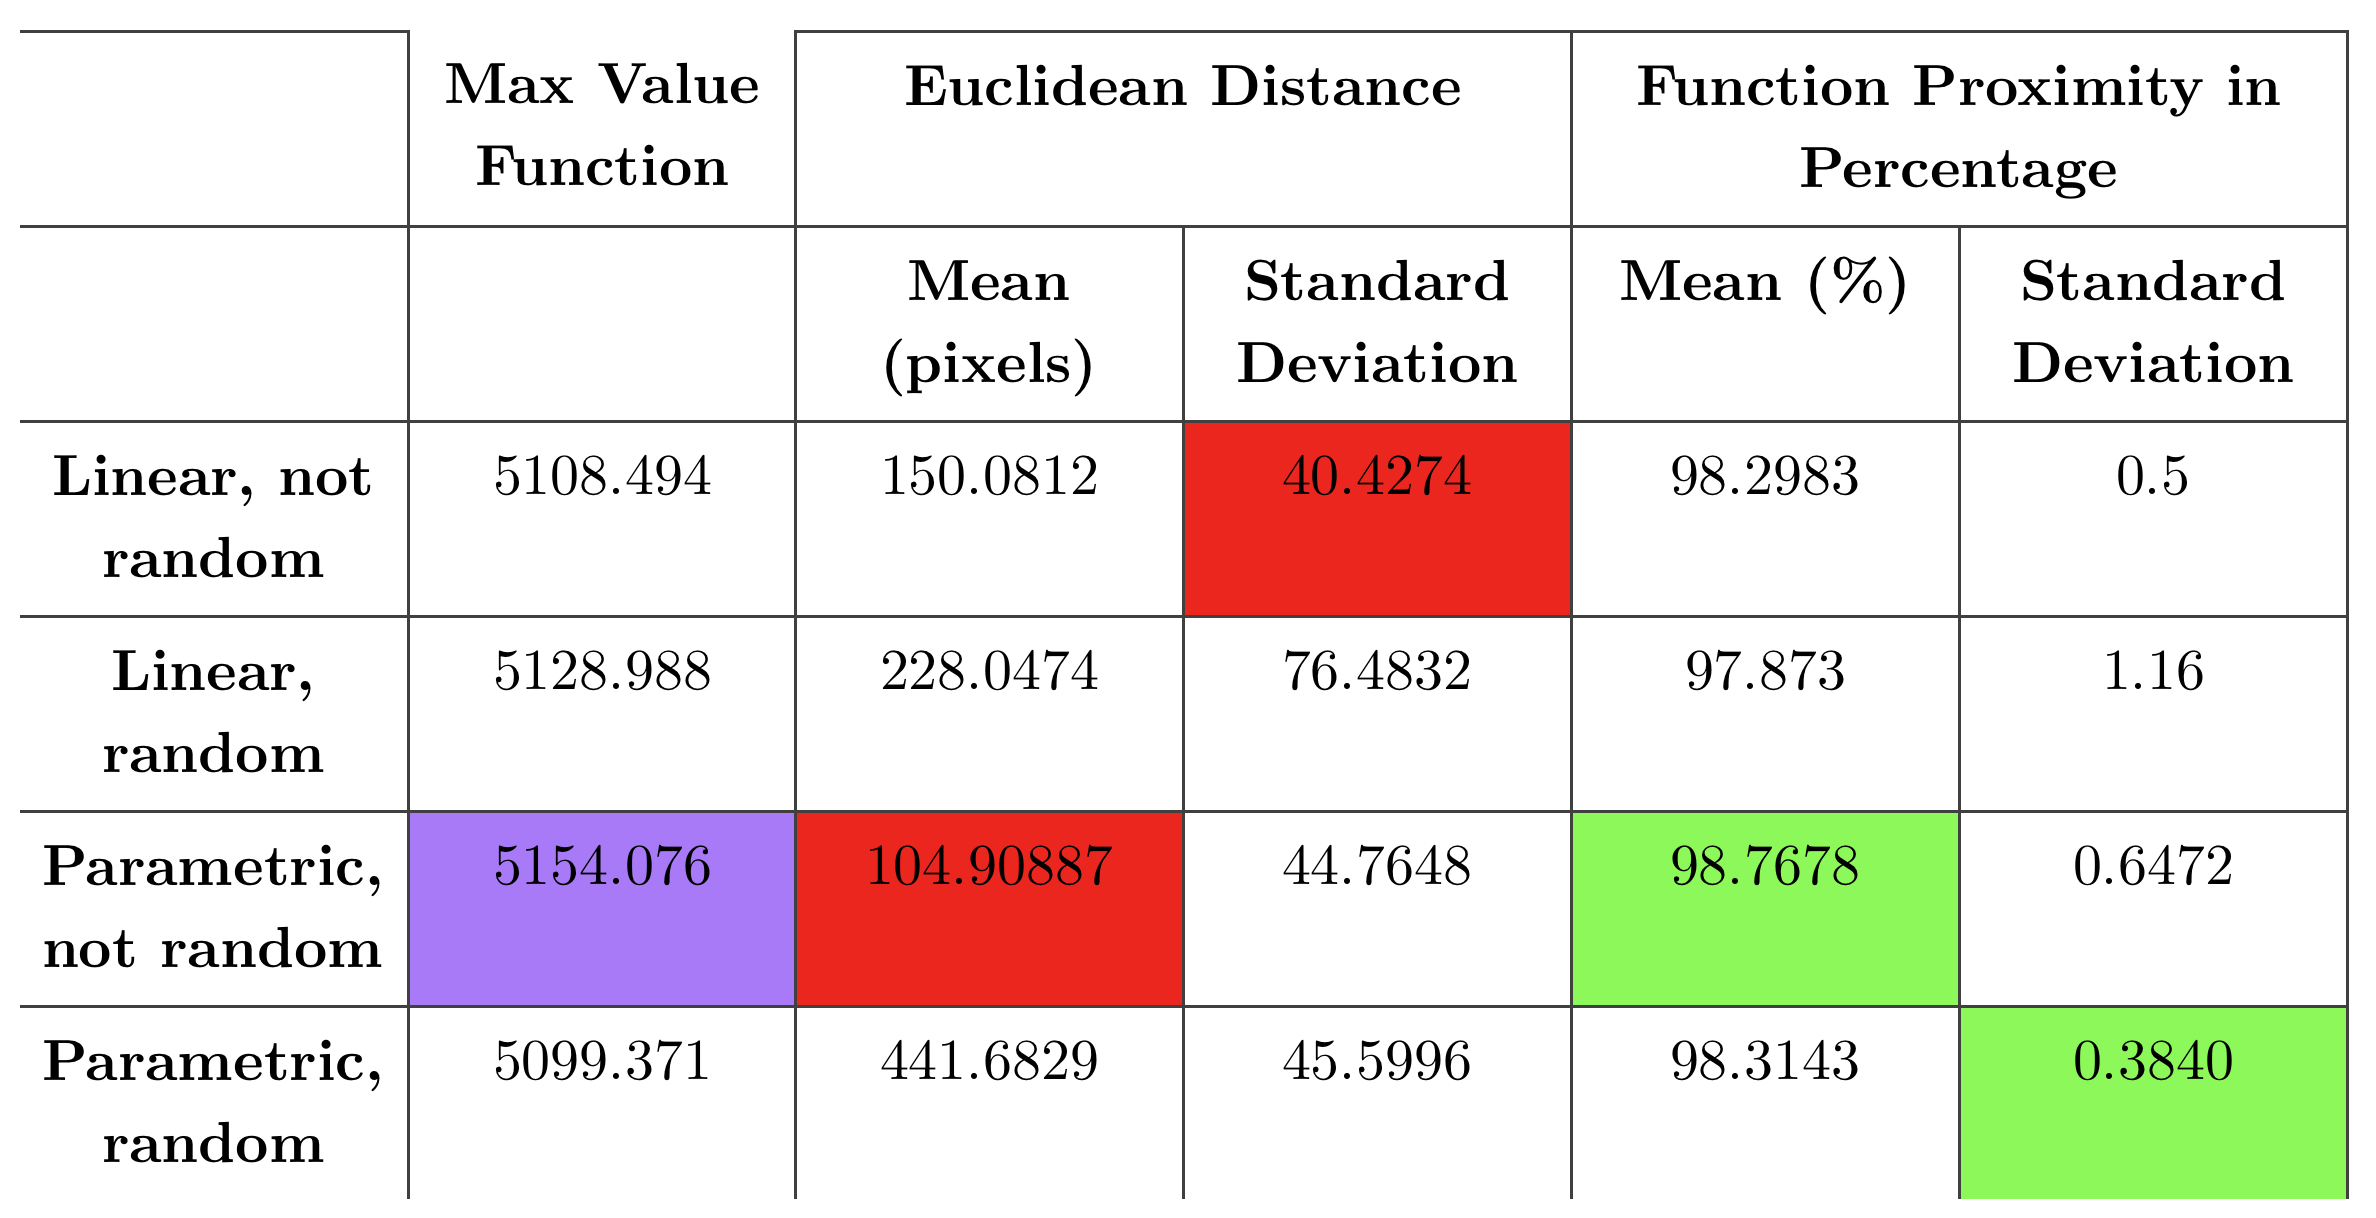
\includegraphics[width=\linewidth]{IMAGES/ExpertReasumingTable}
	\caption{Expert Sarsa($\lambda$)'s Performances Table}
	\label{fig:expertreasumingtable}
\end{figure}
 
The goal of this experiment is to measure how much the \textit{previously acquired experience} from training on different functions, is useful in maximizing a new, never tested before black-box function.

\begin{figure}[h!]
	\begin{center}
		\subfigure[]{%
			\label{fig:StyblinskiDifference}
			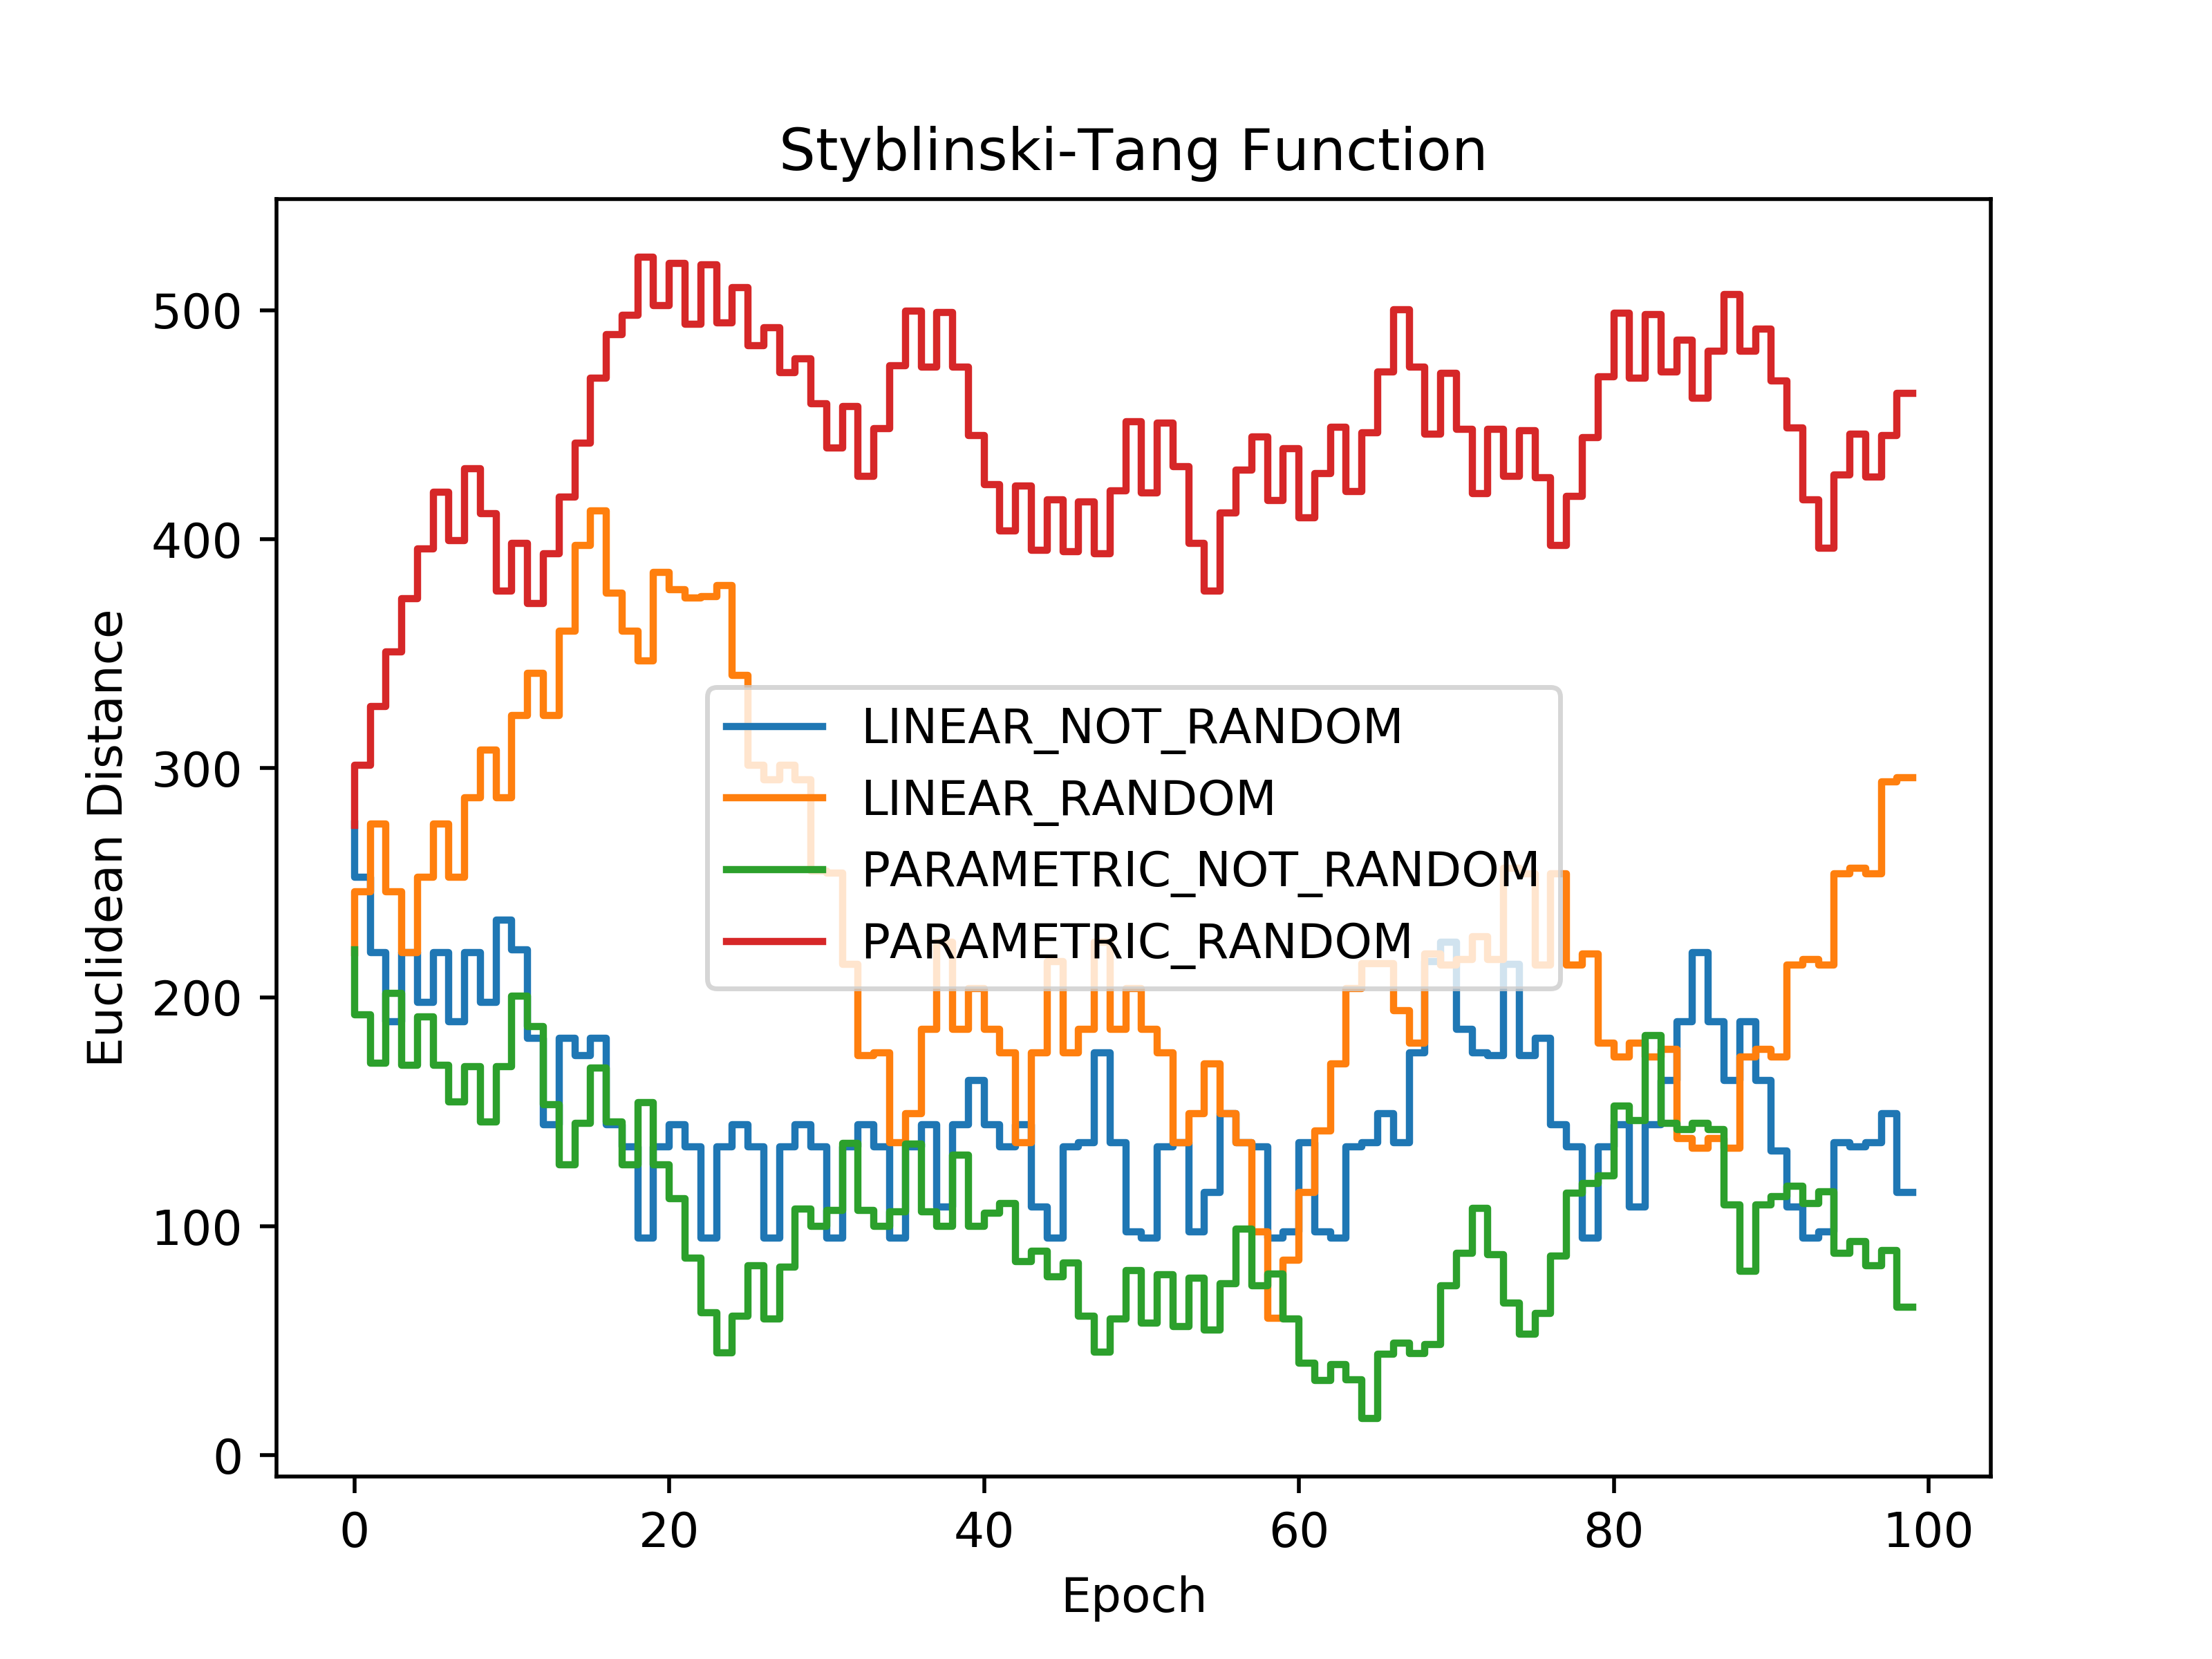
\includegraphics[width=0.4\textwidth]{ExpertStyblinskiDifference}
		}
		\subfigure[]{%
			\label{fig:StyblinskiValueFunction}
			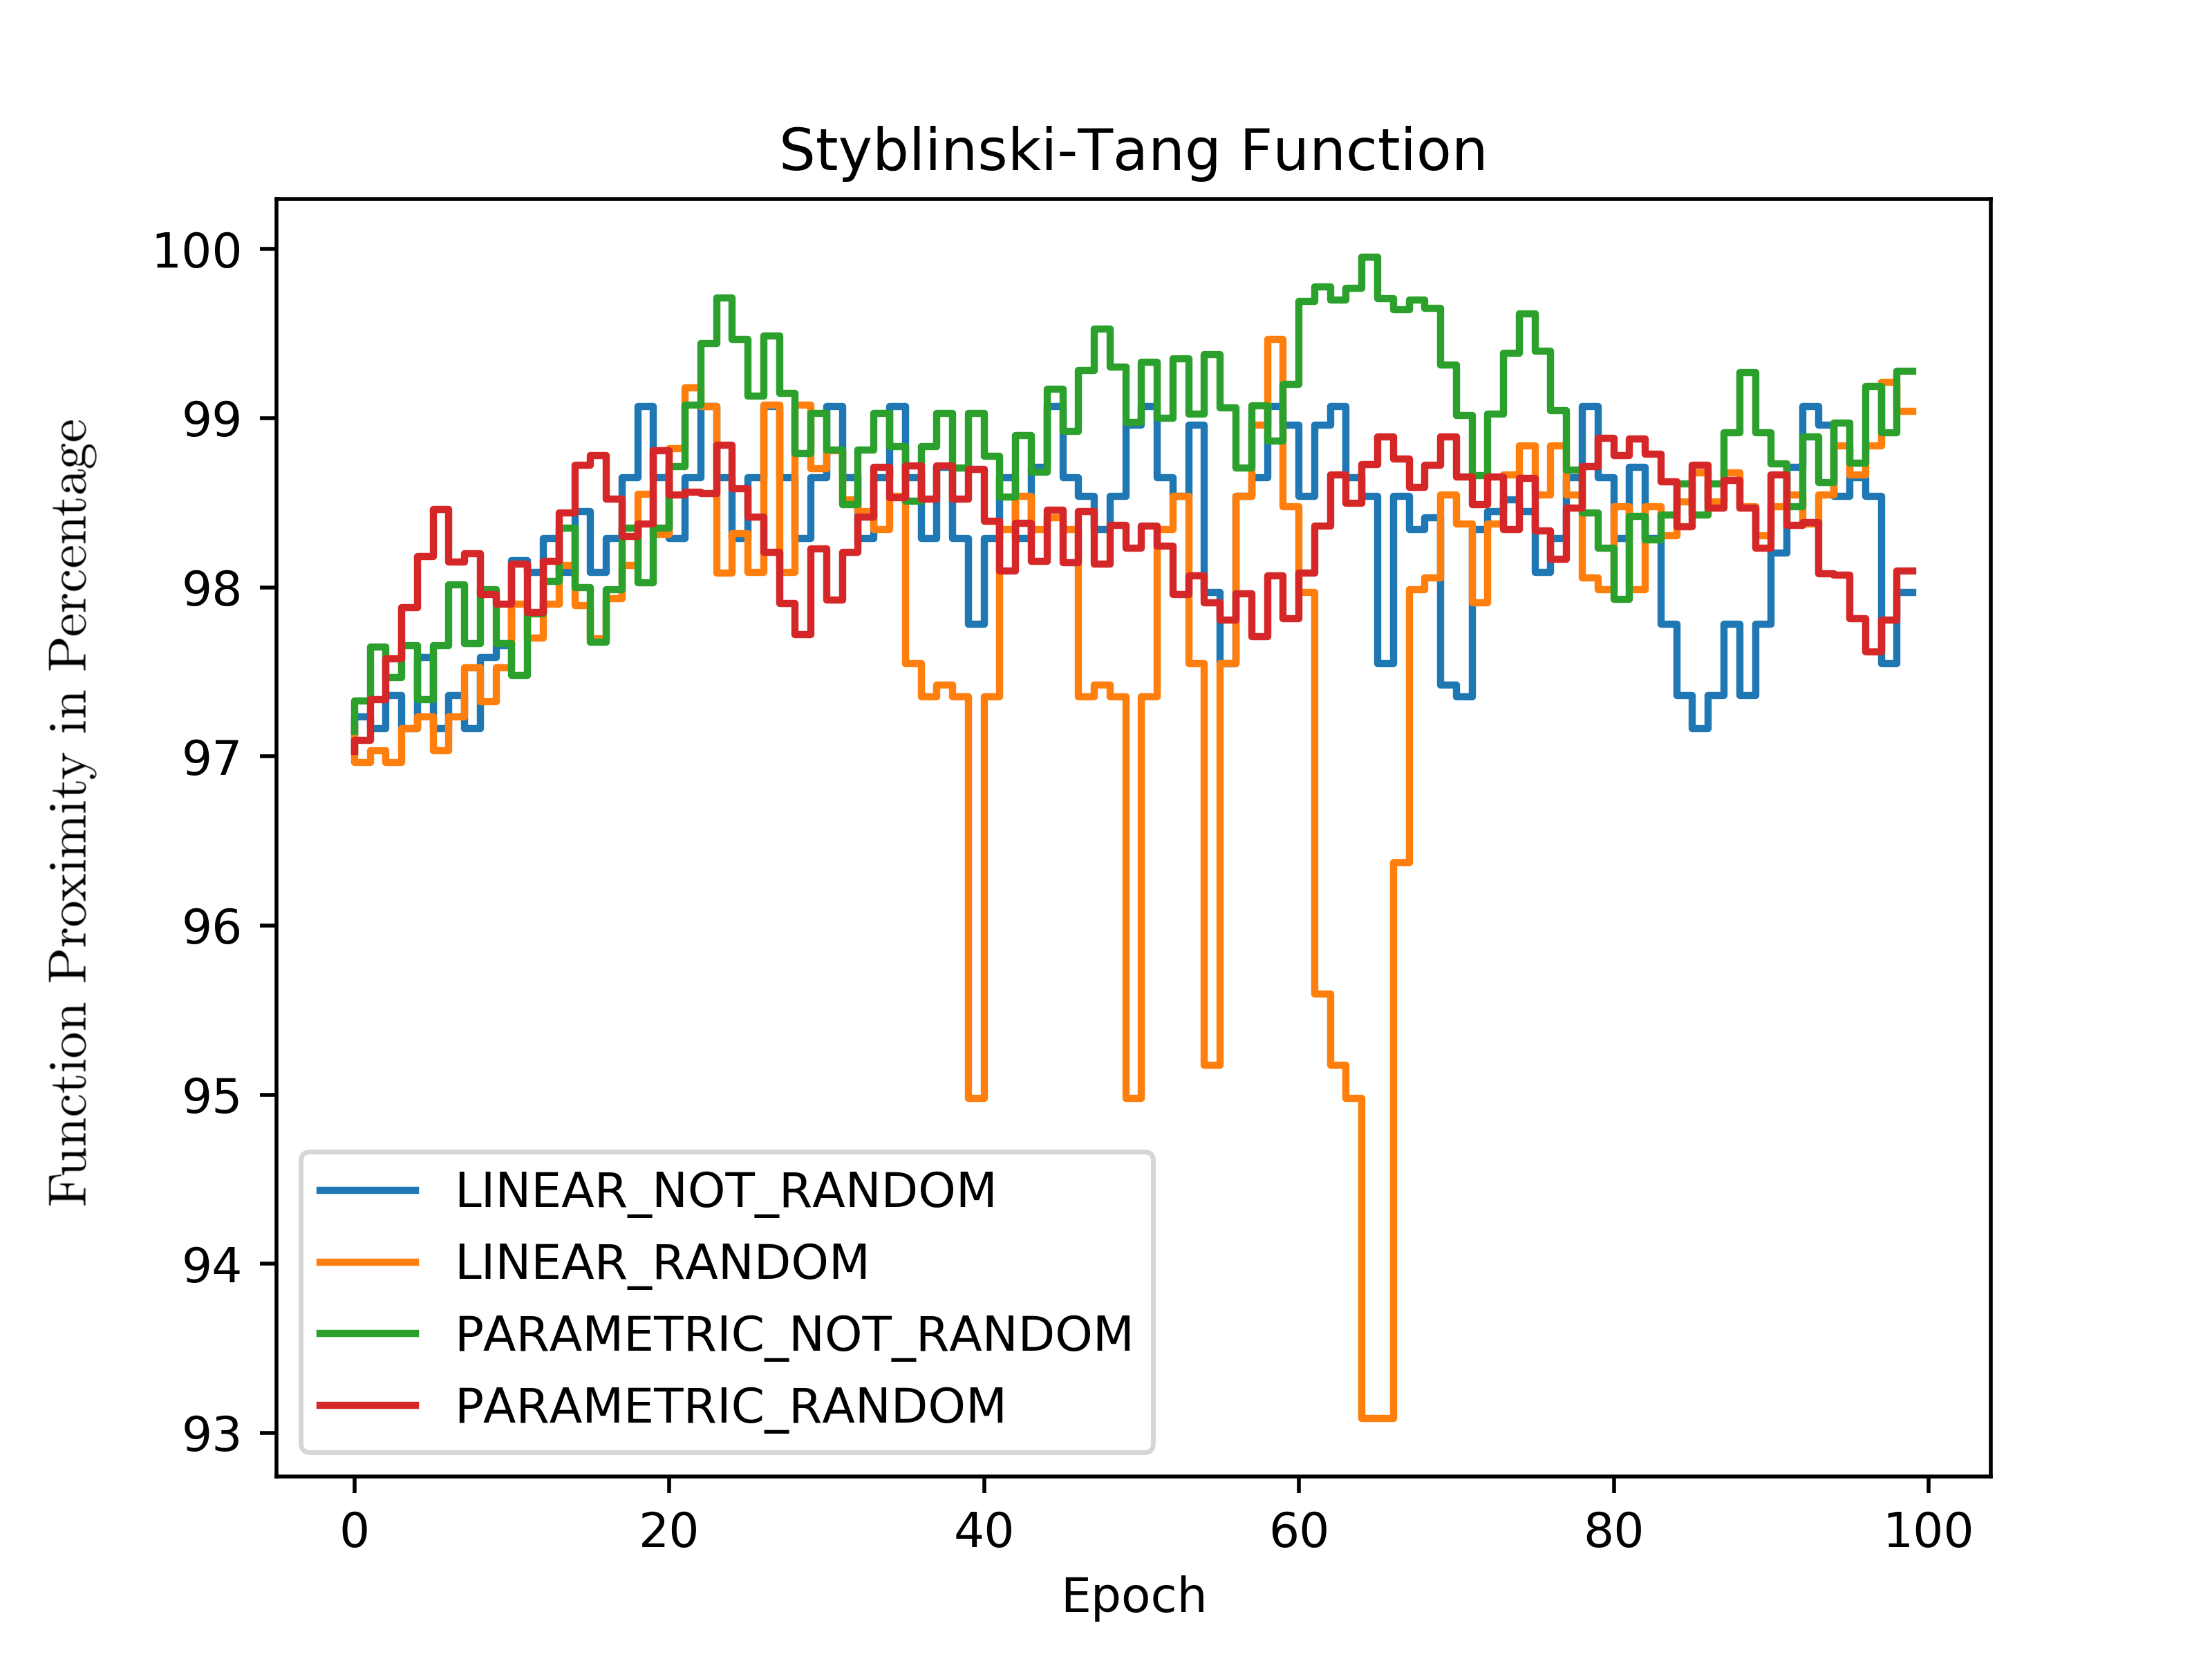
\includegraphics[width=0.4\textwidth]{ExpertStyblinskiValueFunction}
		}\\
		\subfigure[]{%
			\label{fig:StyblinskiGap}
			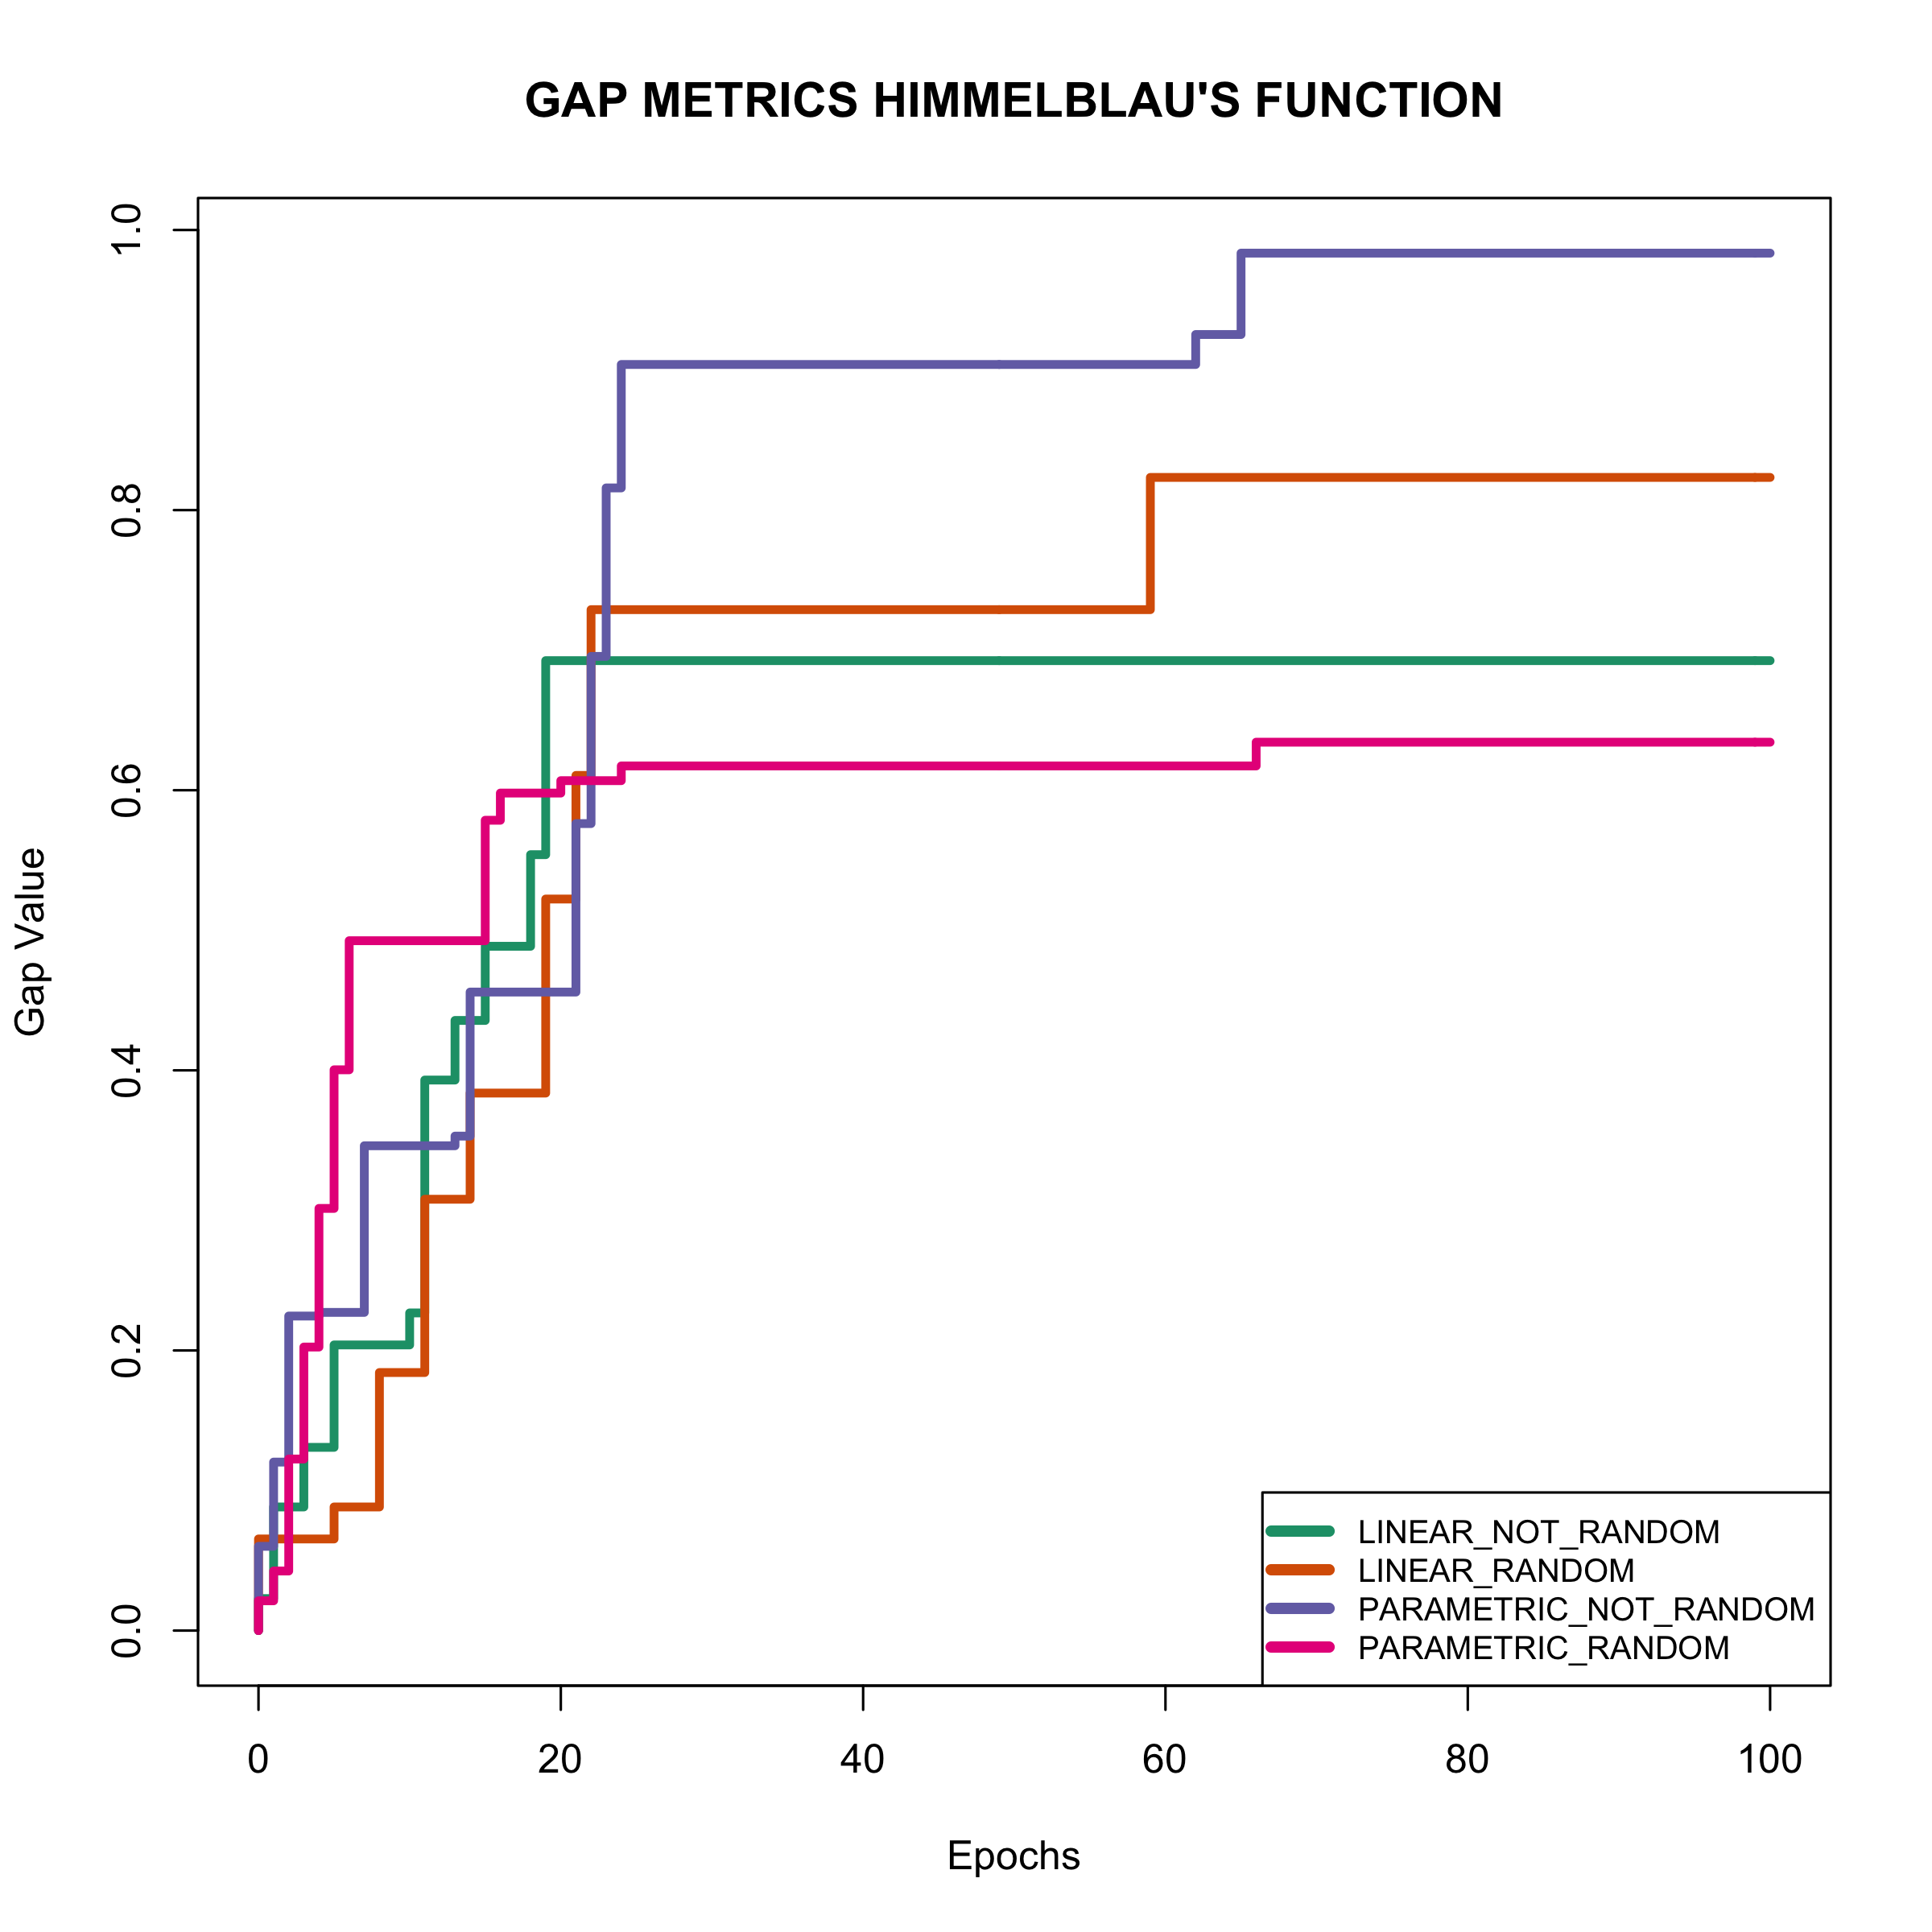
\includegraphics[width=0.4\textwidth]{ExpertGap}
		} \\
		
	\end{center}
	\caption{
		"Expert" SARSA($\lambda$)'s  performances.
	}
	\label{fig:ExpertResults}
\end{figure}

Looking at plot (a) of figure \ref{fig:ExpertResults} it is immediately possible to note that the richest previously acquired experience is given by the {\tt parametric, not random} configuration. In this case, the previously acquired experience on previously tested functions is well expendable with unknown functions. The average Euclidean distance from the maximum in the greedy episode, executed on the never tested function, is equal to $104.90887$ pixels. Despite of this positive value, it is also important to underline the high instability in the same measure. The standard deviation is equal to $44.7648$. The average percentage of value function's proximity to the maximum, is  equal to $98.7678\%$ with a standard deviation of $0.6472$. The general good performance of this declination is confirmed by the fact that the {\tt Gap Value} is the highest between the considered declinations of the employed configuration (plot (c) of figure \ref{fig:ExpertResults}). 

The less reach previously acquired experience is guaranteed by the {\tt parametric, random} configuration. In this case, the Euclidean distance from the maximum constantly swings between $400$ and $500$ pixels. The average Euclidean distance is $441.6829$ pixels with a greater instability certified by the high average standard deviation ($45.5996$) of this measure. Despite of those bad values, it is important to underline that the average percentage of value function's proximity to the maximum is equal to $98.3243\%$ with the lowest standard deviation, which is equal to $0.384$. The general bad performance of this declination is also certified by the lowest {\tt Gap Value} which is equal to $0.6$.

In general, it is possible to say that the two declinations able to guarantee an adequate previously acquired experience useful to maximize black-box, never tested before functions, only running the greedy episode, are the {\tt parametric, not random} declination and the {\tt linear, not random} declination. It is interesting to note that they are both {\tt non random} declinations. It clearly depends on the location of the random starting points during the training phase. Changing the selected seed, those declinations could give better performances.

\section{Humans' Optimization Strategies}

In order to study humans' strategies in the optimization of black-box functions, three acquisition functions are considered :

\begin{itemize}
	\item Upper Confidence Bound ({\tt UCB}) \cite{DBLP:journals/pieee/ShahriariSWAF16}
	\item Probability of Improvement ({\tt PoI}) \cite{DBLP:journals/pieee/ShahriariSWAF16}
	\item Expected Improvement ({\tt EI}) \cite{DBLP:journals/pieee/ShahriariSWAF16}
\end{itemize}

In addition to acquisition functions, also the GP is represented. \\ 

\begin{figure} [h!]
	\centering
	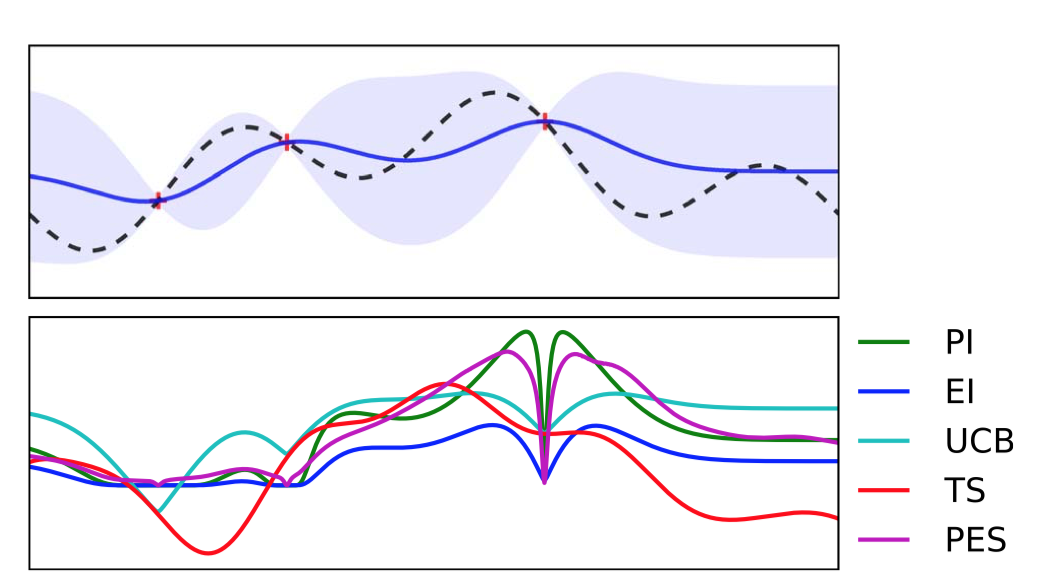
\includegraphics[width=\linewidth]{IMAGES/Surrogate}
	\caption{An example of a GP and associated acquisition functions.}
	\label{fig:surrogate}
\end{figure}

Only the best player's first performance for each function is considered. This means that even if each player has had three possibilities, each one composed of fifteen attempts, for each function (except for the Styblinski-Tang Revised function), only the first one of the three rounds made by the best player for the function itself is here considered. This choice is made in order to study humans' behaviour in the case of no previously experience of the specific function to optimize. The best player is selected according to the highest score reached for each function. In the case there were two best players, the first one's performance is considered.  \\

Results obtained for each function can be found at this link \footnote{\url{https://github.com/AntonioBr/IMAGES/tree/master/HUMANS}} . For each function,  for all the fifteen attempts considered, the first three attempts are employed in order to create the original GP. Starting from the fourth attempt, the white star is employed in order to underline the new attempt chosen by the human compared to the "best" one proposed by the various acquisition functions. Other black points represent previously made attempts. Comparing choices made by human and acquisition functions, it will be clear which one of considered acquisition functions, has led the human in his/her choices.

\subsection{Himmelblau Function}
In the case of the Himmelblau's Function the best player maximizes according to no one on the considered acquisition functions. Looking at the sequence of attempts, the player seems to choose a radically, exploratory approach. All acquisition functions, instead, present a balanced explorative-exploitative approach based on observed data. Looking at the GP obtained at the fifteen attempt, it is possible to note that the original, black-box function is well approximated.

\subsection{Sphere Function}
In the case of the Sphere Function the best player maximizes according to {\tt PoI} acquisition function. The process to achieve the maximum is linear and the player never try a radical different exploratory attempt. The GP well approximates the real, black-box function still starting from the sixtieth attempt.

\subsection{Beale Function}
In the case of the Beale Function the best player maximizes according to {\tt PoI} acquisition function until the sixtieth attempt. Starting from the seventh attempt it maximizes according to {\tt UCB} acquisition function till the fifteenth attempt. After fifteen attempts, the GP does not well approximate the real, hidden function, but isolates the region of the maximum.

\subsection{Styblinski Revised Function}
The case of the Styblinski revised function is surely the most interesting one. By default, the best player can make only one round composed by fifteen attempts. The best player is here defined just according to its only, experience-free set of attempts. In this case the best player maximizes according to the {\tt UCB} acquisition function. Also in this case, after fifteen attempts the GP does not well approximate the real, black-box function, but isolates the region of the maximum. This means that the player did not make enough exploration. It is interesting to note how it is possible to identify an acquisition function corresponding to the human reasoning process, considering that it was not possible in the case of the Himmelblau's Function. It is also interesting to note how the best player in this case is different from the one of the Himmelblau Function. The two functions were selected because of their shapes' similarity. Results obtained are different for the two similar functions. \\

In the $100\%$ of cases, best players are male. Their mathematical knowledge level is in the $100\%$ of cases the highest possible. They are all test subjects with an age between $19$ and $22$.

\section{RL Agent's  policy vs Humans' Strategies}
All experiments described in the previous sections are useful to better understand the one described in the current section. As previously said, one of the main goals of this thesis is comparing humans' strategies with the policy adopted by a RL agent in the optimization of black-box $2d$-functions. In order to do this, it has been considered the case of maximization of Styblinski-Tang' s Revised Function. In the previous section, humans' strategy with no previously acquired knowledge about a specific function, has been studied. Making the same study on performances of a RL agent could be not very fruitful because of the great amount of training required by the algorithm in order to obtain acceptable results. Despite of this, a good choice is to compare humans' performances and RL agent's ones in the case of maximization of black-box $2d$-functions with \textit{previously acquired experience}. To be more specific, when one of the human test subjects, maximizes the Styblinski-Tang's Revised Function, he/she has already had experience with optimization of Himmelblau's Function, Sphere Function, Beale Function. The same is for the RL agent in the case of the \enquote{Experienced} SARSA($\lambda$) algorithm.

In the human case, the best player optimizes according to the {\tt UCB} acquisition function. After fifteen attempts the GP does not well approximate the real, black-box function, but isolates the region of the maximum. The case of RL agent is more complex. As seen in the plots of figure \ref{fig:ExpertResults}, the {\tt parametric, not random} declination is the one with the best performances. The RL agent which operates according to this declination, doesn't optimize according to a specific acquisition function until epoch $60$ (figures can be found at this link \footnote{\url{https://github.com/AntonioBr/IMAGES/tree/master/EXPERIENCED SARSA LAMBDA}}). Starting from the sixtieth epoch, it optimizes according both to the {\tt UCB} acquisition function, and, more rarely, according to the {\tt PoI} acquisition functions. At the end of the $101$ epochs of the unique episode run on the Styblinski-Tang's Revised Function, the GP developed starting from performances obtained by the RL agent, better approximates the real, hidden function if compared with the case of the GP developed starting from the human performances. \\

Those results can be explained as follow. The RL based, optimization process is slower (and apparently less accurate) than humans' one because of limits imposed by the definition of the agent, e.g. the limited amount of movement for each epoch and the movement schema, and because of the absence of \textit{intuition}. Despite of this RL based optimization approach' s deficit, it is very interesting to note how the subtended acquisition function could sometimes be the same for the RL agent and humans in the optimization of the same black-box $2d$-function. 



	\chapter{Appendix A}

One of the most amazing aspect of the work presented in this thesis is the manner in which the goal has been reached. I want to clarify that during the first weeks, it was not easy to understand the real target of the work. This initial uncertainty led us to implement some strange solutions. Even if some of these approaches were not useful for the goal described in the previous chapters of this thesis, although they were very efficient in different contexts. For this reason we will here recall the full history of the current research activity. In so doing, we identify ten different main steps. 

\paragraph{First Step} In the first attempt to reach the solution of the problem, we allowed the agent to take five different actions :

\begin{itemize}
	\item Move North
	\item Move South
	\item Move West
	\item Move East
	\item Dig.
\end{itemize}

In so doing, we distinguished between the possibility for the agent to take a \textit{movement action} or a \textit{dig action}. In this choice we were inspired by the possibility for humans to make movements for no specific reason. We later understood that this implementation was redundant. Humans move themselves for no apparently reason before decide to take a goal-directed action. A RL agent \textit{decides} what action taking in the next step immediately after have completed the previous action without needing \textit{time to think}. \\

In this step the state was represented by three elements :

\begin{itemize}
	\item Coordinate $x$
	\item Coordinate $y$
	\item Number of remaining \textit{function soundings}
\end{itemize}

Unfortunately such a state representation prevents from the possibility to generalize the training. Given two different bivariate functions $f(x, y)$ and $g(x, y)$ and supposing to have trained the RL agent using function $f(x, y)$, when we decide to sound $g(x, y)$ on point $x$ and $y$ already sounded in $f(x, y)$, the result could be different (figure ~\ref{fig:ComparisonBetweenTwoFunctions}).

\begin{figure}[h!]
	\begin{center}
		\subfigure[$f(x, y) = 2xy$, \quad $f(1, 1) = 2$]{%
			\label{fig:2xy}
			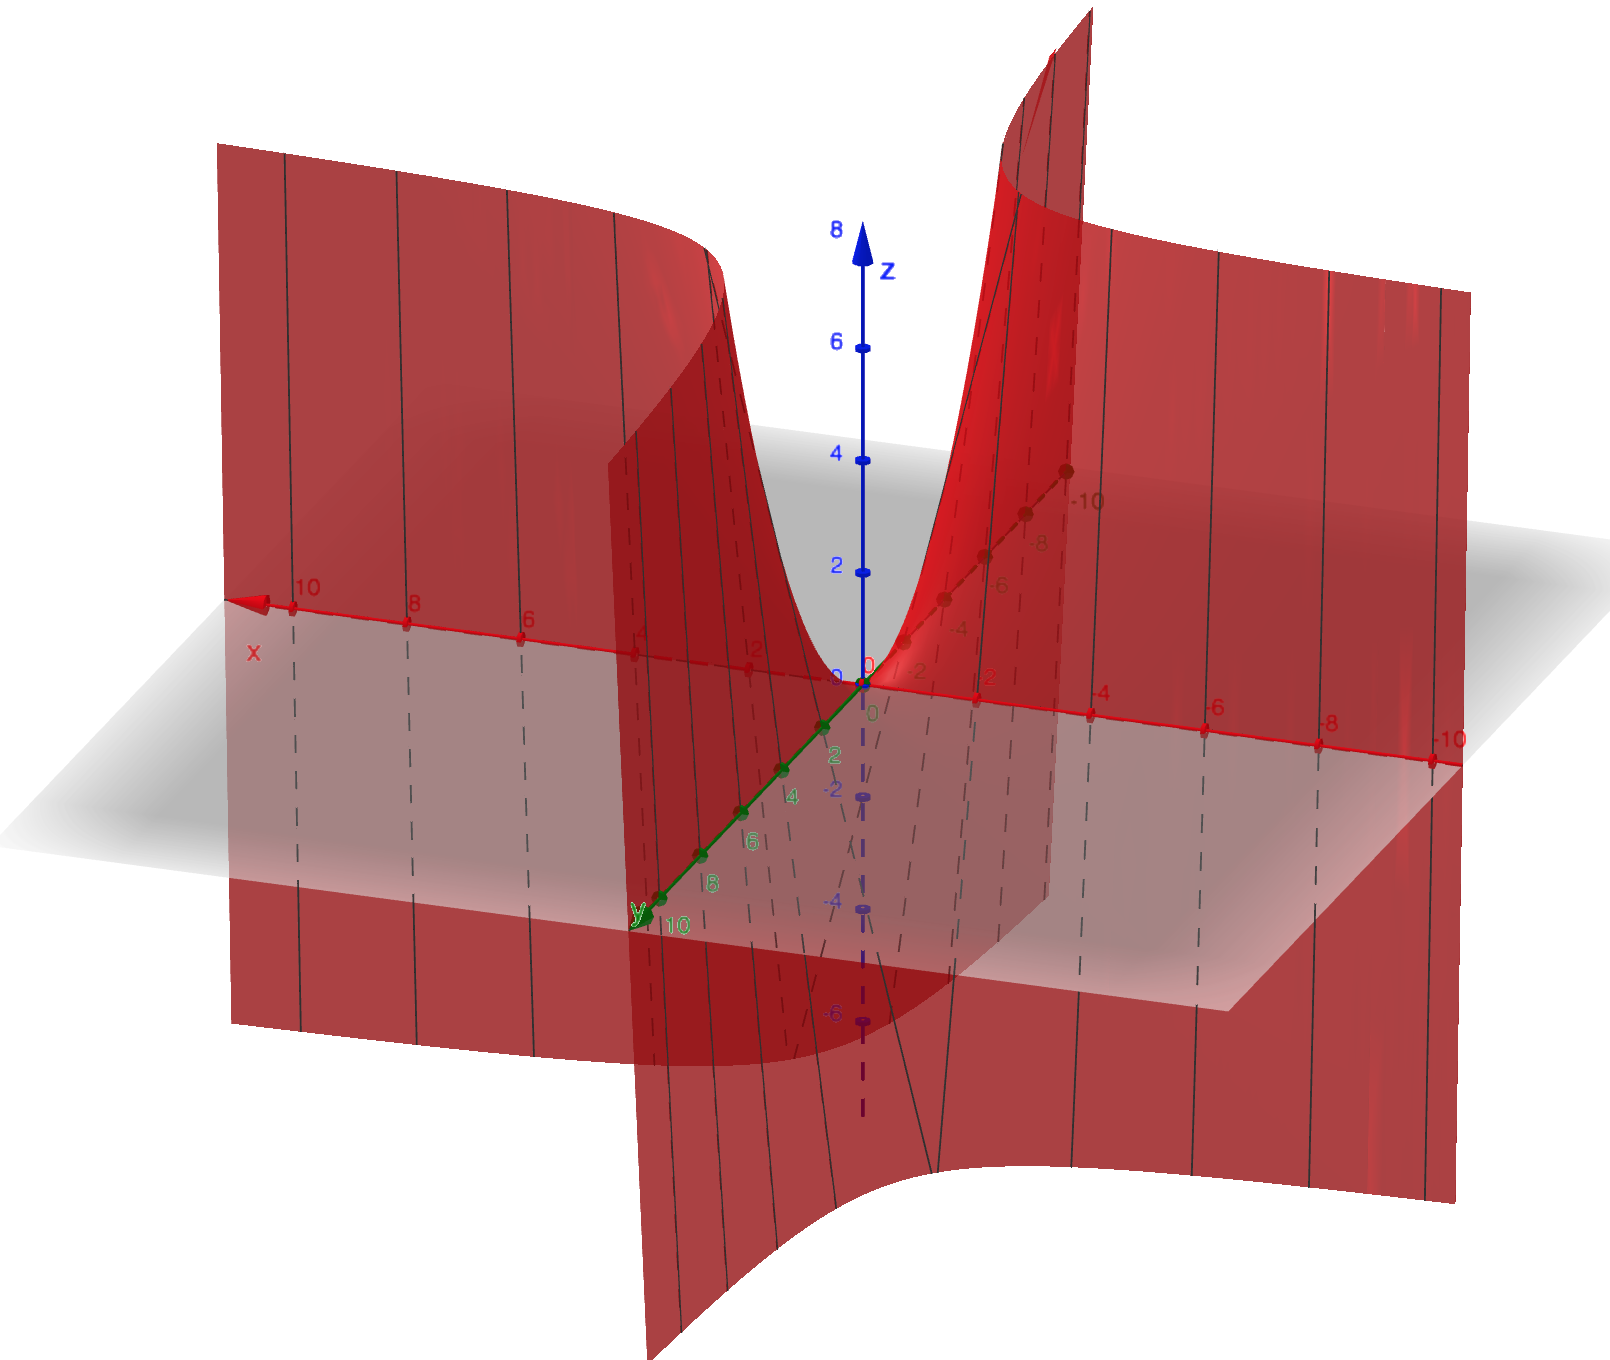
\includegraphics[width=0.4\textwidth]{2xy}
		}
		\subfigure[$g(x, y) = xsin(y)$, \quad $g(1, 1) = 0.017$]{%
			\label{fig:xsin(y)}
			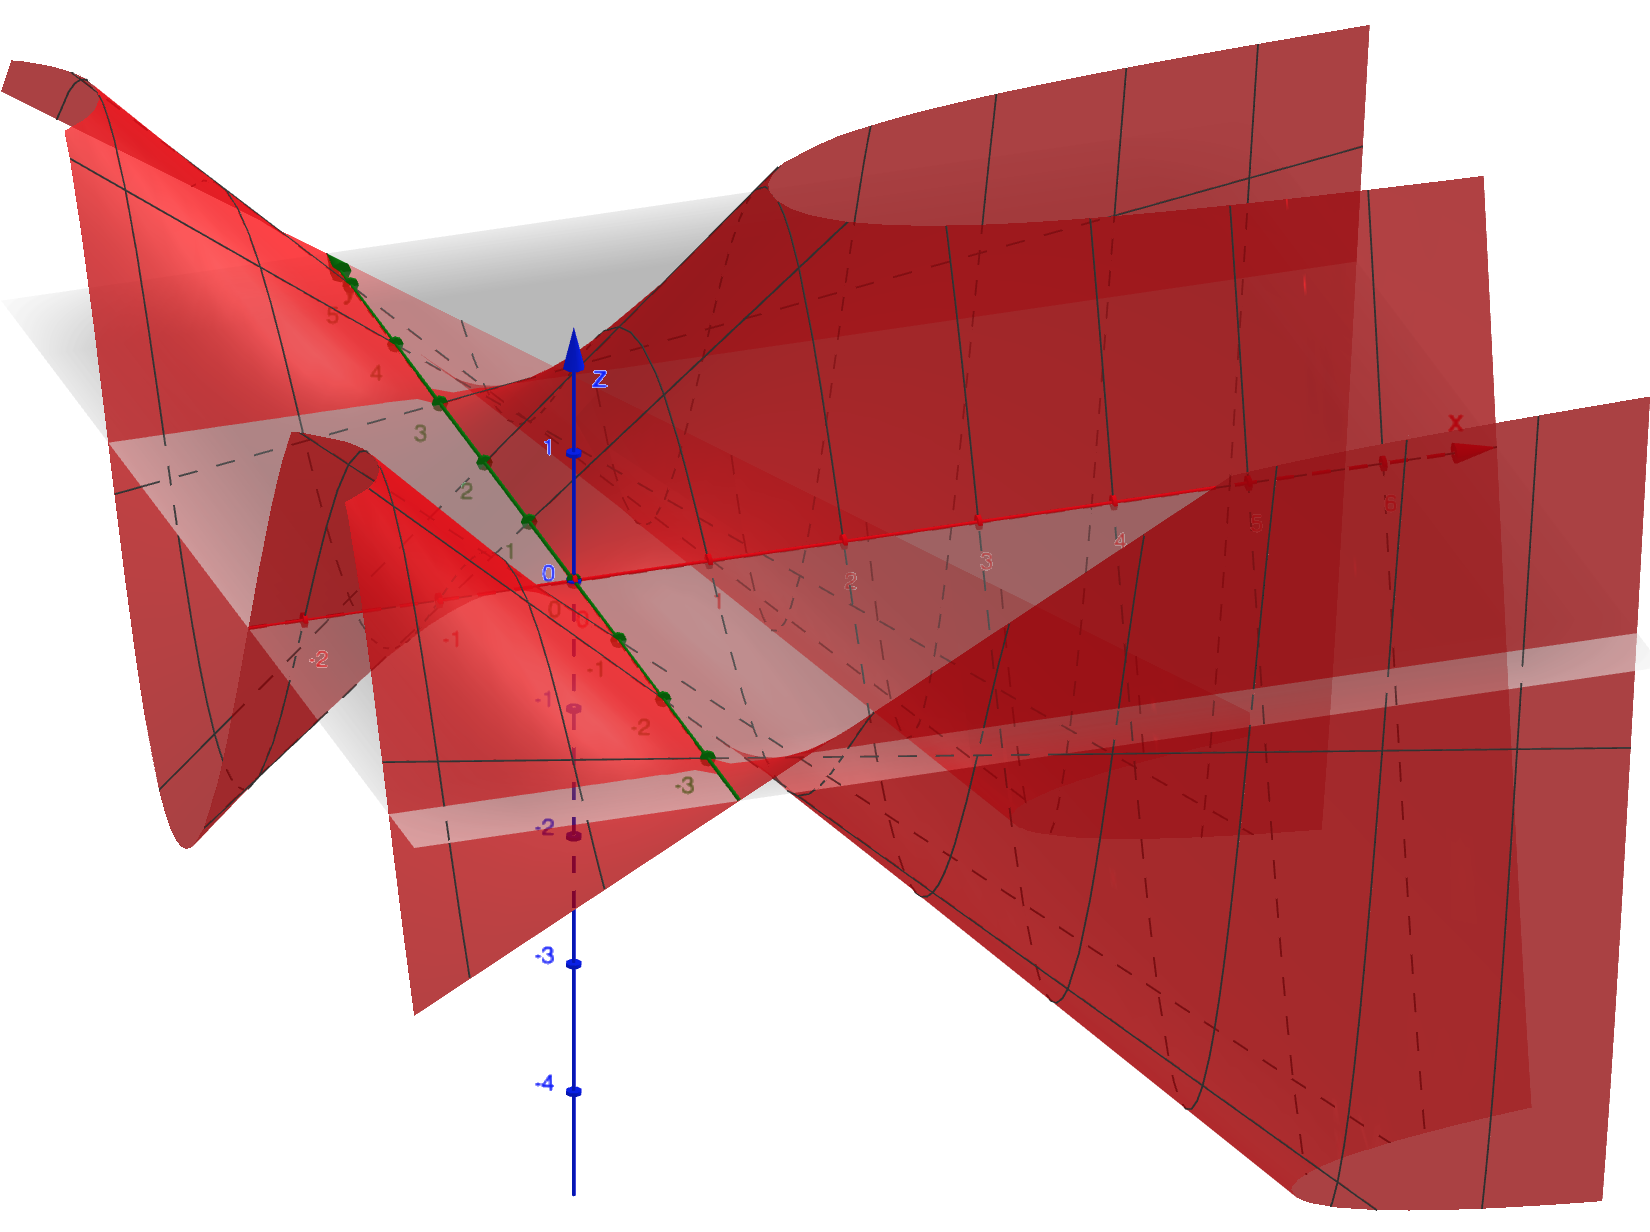
\includegraphics[width=0.4\textwidth]{xsin(y)}
		}
	\end{center}
	\caption{
		Different value functions for different functions.
	}
	\label{fig:ComparisonBetweenTwoFunctions}
\end{figure}

In addition to this, we soon understood that the information concerning the number of remaining function' s soundings is redundant. It did not add any information to our knowledge. 
In the implementation described above, the agent was in a terminal state when the number of remaining function soundings was equal to zero.

\paragraph{Second Step} The second step was globally equal to the first one except for two fundamental aspects. In the current step we introduced the possibility for the agent to make movements of different sizes. This possibility allowed its to reach the goal with a lower training time. 

We also redefined the reward function. It was equal to the percentage of proximity to the maximum of the function. Soon we understood that a so defined reward function was completely wrong. In a context of black-box optimization the maximum of the function is unknown and we are unable to compute the percentage of proximity to the maximum.

\paragraph{Third Step} In the third step we made an additionally change to the previous one. At the end of each episode, the agent was artificially forced to restart from the coordinates of the previous episode's best rewarded epoch. Results given by the combination of the last two approaches resulted to be very fruitful in the context well-known function optimization but not in the context described in this thesis. Indeed we are forcing the agent to take a specific action, breaking, in so doing, for at least one time the concept of environment formalized through a Markov Decision Process.

\paragraph{Fourth Step} In the fourth step we improved the performance obtained through changes made in the second and third step. We succeeded in so doing, imposing the agent to start each episode from the best rewarded epoch from all previous episodes.

\paragraph{Fifth Step} The fifth step is one of the most important because of innovations introduced starting from its. The first change made regards actions. In this step we introduced the possibility for the agent to directly choose the size of the movement. There are still four different possible \textit{movement actions} :

\begin{itemize}
	\item Move North
	\item Move South
	\item Move West
	\item Move East
\end{itemize}

but the agent could select to move itself in one direction of :

\begin{itemize}
	\item \textit{movement amount};
	\item \textit{movement amount} $\times 2$;
	\item \textit{movement amount} $\times 3$.
\end{itemize}

Remember that the unit of measurement of \textit{movement amount} is the \textit{pixel}. The basic amount of movement is 40 pixels. The real movement amount over function is computed through algorithm \ref{algoPixel} in Chapter $3$. It was proved that using this set of \textit{action movements} the algorithm converged more quickly to the maximum of the function but the precision was lower. 

In addition to this, we have also removed the possibility for the agent to distinguish between \textit{move action} and \textit{dig action}. Each time the agent made a movement it also sounded the function obtaining a reward. The reward was positive if its proximity to the global maximum was in percentage $\ge 75\%$, negative in other cases. As already explained, the disadvantage of the last choice is that in the context described in this thesis the objective function is unknown so we are not able to compute the percentage of proximity to the maximum.

\paragraph{Sixth Step} In this step we introduced the concept of \textit{delta}. \textit{delta} was computed as the difference between the value of the function sounded at time $t$ and the maximum value sounded until time $t$. 

In this step we also tried to reach an higher control about \textit{exploration} and \textit{exploitation}. In order to do this we introduced a decreasing $\epsilon$ factor between episodes. We tried different decreasing functions and we noticed that the best one was the logarithmic one. 

In this step the reward was still based on the concept of percentage with an engagement of the \textit{delta}. To be more specific if the \textit{delta} was $\le 0$ or the percentage was $\le 78$ the reward was negative, otherwise it was positive.

\paragraph{Seventh Step} In this step we improved the definition of the reward function. We removed the concept of percentage of proximity to maximum and we introduced a reward based exclusively on the difference between the sounded value function at time $t$ and the maximum until time $t$. This was a little but fundamental adjustment because it removed a relevant mistake from the project.

\paragraph{Eighth Step} We can define this step as an experimental step. Here we focused on the possibility to make the agent able to explore more. In order to do this we introduced the possibility to start each episode from a random point. Through this experiment we proved that more exploration gave the possibility to prevent many limit cases but it did not always entail an improvement in algorithm performances in terms of time and precision.

\paragraph{Ninth Step} The current one is the second revolutionary step. It introduces two innovative elements: the \textit{parametric movement} and the \textit{stop action}.
As explained in chapter $3$, the parametric movement allows to compute the \textit{real agent's movement amount} keeping in consideration an approximation of function' s shape.

Speaking about the second innovation introduced,  we have to say that when \textit{stop action} was selected, the simulation of the current episode was interrupted. Consequences from introduction of this new action were very interesting. Given a inadequate training space, the \textit{stop action} led to an immediate stop. This depended on the fact that rather than receiving more negative rewards before reaching a maximum better than the current one (i.e. the starting point itself), it computed that the optimal policy consisted in staying around the starting point itself, still moving according to a recurring pattern that minimizes the negative rewards.

\paragraph{Tenth Step} This represents the last step before the final version of the project. In this version the state was revolutionised. It was now composed of the last three angles of improvements computed as described in chapter $3$. Angles varied between $- \pi$ and $+ \pi$ because also a worsening is here considered. Angles were rounded to the nearest multiple of two. The choices introduced in this step were unexpectedly not fruitful. The failure depended on two factors. Last three angles as the unique component of the state were not enough and the rounding cannot be chosen a priori. The correct choice of rounding should depend on the \textit{Lipschitz Constant}. 

Let's consider a single-variable function $f(x)$ for $x$ inside a domain $D$. The magnitude of the slope of $f(x)$ for two points $(x_1, f(x_1))$ and $(x_2, f(x_2))$ is thus 

\begin{equation}
	|\dfrac{f(x_1)-f(x_2)}{x_1 - x_2}|.
\end{equation}

A non-negative real number $L$, which is the smallest upper bound of the slope is called the \textit{Lipschitz Constant} :

\begin{equation}
L = |\dfrac{f(x_1)-f(x_2)}{x_1 - x_2}| = sup|\dfrac{df}{dx}|.
\end{equation}

The Lipschitz Constant limits how fast the function can change. If there is no Lipschitz Constant, the function can change extremely fast without border, that is, the function becomes discontinuous\cite{Lipschitz}.

For multivariate function the \textit{Lipschitz Constant} is defined as:

\begin{equation}
L\textsubscript{x\textsubscript{n}} = sup|\dfrac{\partial f}{\partial x_n}|.
\end{equation}

\begin{figure} [h!]
	\centering
	\includegraphics[width= 10cm, height = 10cm]{Lipschitz.png}
	\caption{Let's consider a $1d$-function $f(x) = x^2$ defined in the domain $x \in [0, 2]$. If $|\frac{df}{dx} f(x) | = 2x$, then $L = \sup |\frac{df}{dx}| = 2 \times 2 = 4$.}
	\label{fig:Lipschitz}
\end{figure}


	\includepdf[pages=-]{EXTRA/Grafici}
	\chapter*{Acknowledgements}
\pagestyle{empty}

First of all, I wish to thank my supervisor, Dr. Antonio Candelieri for his help, for his advices and for his limitless patience during my period of internship. I am indebted with him for the calculation of the acquisition functions employed by humans in their optimization process. \\

I wish to thank my family and my parents Maria and Donato for their support. I would like to thank in particular my sister Giusy for her help in conducting tests on humans. \\

I would also like to thank Cristian Baldi, Demetrio Carrara, Fabio Cimmino, Marco Palmiero, Cezar Sas and Silvia Terragni for four months reach of many useful discussions. \\

Finally, I would like to thank Lorenzo, Daniele, Nicolò, Simone  and all other friends for the laughs during the period of studies. \\

The research described in this thesis was carried while I held a research internship from the MIND Laboratory of University of Milan, Bicocca. \\

\flushright{$12$th July 2018}\flushright{Antonio Briola}
	
	\bibliography{bibfile.bib}
	\bibliographystyle{alpha}
	
\end{document}
